 \documentclass[oneside,11pt]{article}


\usepackage{soul}
\usepackage{natbib}
\usepackage{hyperref}
\usepackage{bookmark}
\usepackage{graphicx}             
\graphicspath{{./Figuras/}}
\usepackage[dvipsnames]{xcolor}
\usepackage{todonotes}
\usepackage{makecell}
\usepackage[margin=1in]{geometry}
\usepackage{float}                
\usepackage{amsmath}
\usepackage{amscd}
\usepackage{amsfonts}
\usepackage{amssymb}
\usepackage{bbm}
\usepackage{booktabs}
\usepackage{nameref}
\usepackage{multirow}
\usepackage[nokeyprefix]{refstyle}
\usepackage{rotating}
\usepackage{threeparttable}
\usepackage{afterpage}
\usepackage{lscape}
\usepackage{enumerate}
\usepackage{caption}
\usepackage{subcaption}
\usepackage{epstopdf}
\usepackage{setspace}
\usepackage{svg}
\usepackage{dsfont}
\usepackage{amsthm}
\usepackage{tocloft}
\usepackage{etoc}
\usepackage{lmodern}
\usepackage{bm}
\usepackage[T1]{fontenc}
\usepackage{tgpagella}

\epstopdfDeclareGraphicsRule{.tiff}{png}{.png}{convert #1 \OutputFile}
\AppendGraphicsExtensions{.tiff}

\epstopdfDeclareGraphicsRule{.tif}{png}{.png}{convert #1 \OutputFile}
\AppendGraphicsExtensions{.tif}

\def\sym#1{\ifmmode^{#1}\else\(^{#1}\)\fi}

\usepackage{tikz}
\usetikzlibrary{shapes.geometric, arrows}
\usetikzlibrary{calc}
\usetikzlibrary{matrix}

\tikzset{ 
    table/.style={
        matrix of nodes,
        row sep=-\pgflinewidth,
        column sep=-\pgflinewidth,
        nodes={
            rectangle,
            draw=black,
            align=center
        },
        minimum height=1.5em,
        text depth=0.5ex,
        text height=2ex,
        nodes in empty cells,
%%
        every even row/.style={
            nodes={fill=gray!20}
        },
        column 1/.style={
            nodes={text width=2em,font=\bfseries}
        },
        row 1/.style={
            nodes={
                fill=black,
                text=white,
                font=\bfseries
            }
        }
    }
}


\usepackage{colortbl}
\usepackage{url}
\urlstyle{rm}
\definecolor{darkblue}{rgb}{0,0,.4}
\hypersetup{colorlinks=true, breaklinks=true, citecolor=Maroon, linkcolor=darkblue, menucolor=darkblue, urlcolor=darkblue}

\newtheorem{theorem}{Theorem}
\newtheorem{claim}[theorem]{Claim}
\newtheorem{prop}[theorem]{Proposition} 
\newtheorem{cor}[theorem]{Corollary} 
\newtheorem{assumption}{Assumption} 
\newtheorem{lem}{Lemma} 

\DeclareRobustCommand{\hlgr}[1]{{\sethlcolor{green}\hl{#1}}}


\usepackage{comment}
%para esconder columnas en tablas (enrique)
\usepackage{array}
\newcolumntype{H}{>{\setbox0=\hbox\bgroup}c<{\egroup}@{}}
\linespread{1.25}

\newcommand{\wh}{\widehat}
\usepackage{anyfontsize}

\usepackage[linesnumbered,vlined,ruled,commentsnumbered]{algorithm2e}

\DontPrintSemicolon
\newcommand{\To}{\mbox{\upshape\bfseries to}}
\newcommand{\E}{\mathbb{E}}

\DeclareCaptionFormat{cont}{#1 (cont.)#2#3\par}
%%% HELPER CODE FOR DEALING WITH EXTERNAL REFERENCES
\usepackage{xr}
\makeatletter
\newcommand*{\addFileDependency}[1]{
  \typeout{(#1)}
  \@addtofilelist{#1}
  \IfFileExists{#1}{}{\typeout{No file #1.}}
}
\makeatother


\newcommand*{\myexternaldocument}[1]{
    \externaldocument{#1}
    \addFileDependency{#1.tex}
    \addFileDependency{#1.aux}
}

%\myexternaldocument{OA}

%%%%%%%%%%%%%%%%%%%%%%%%%%%%%%%% DOCUMENT
\begin{document}

%----------------------------------------------------------------------------------------
%	PORTADA
%----------------------------------------------------------------------------------------

\begin{titlepage}
\begin{center}

\title{RPCI}

\textsc{\Large Instituto Tecnológico Autónomo de México}\\[2em]

%Figura
\begin{figure}[h]
\begin{center}

\includegraphics[scale=0.50]{04_Figures/itam_logo.png}
\end{center}
\end{figure}

% Pueden modificar el tamaño del logo cambiando la escala

\textbf{\LARGE The effect of information in improving payroll compliance}\\[2em]

\textsc{\large Tesis}\\[1em]

\textsc{\large que para obtener el título de}\\[1em]

\textsc{\LARGE Licenciado en Economía}\\[1em]

\textsc{\large Presenta}\\[1em]

\textsc{\LARGE Marco Alejandro Medina Salgado}\\[1em]

\textsc{\large Asesor}\\[1em]

\textsc{\LARGE Dr. Enrique Seira Bejarano}\\[2em]

% Asegúrense de escribir el nombre completo de su asesor

\end{center}

\vspace*{\fill}
\textsc{Ciudad de México \hspace*{\fill} 2023}

\end{titlepage}

%\vspace{.5in}


%\maketitle
%\thispagestyle{empty}
%\begin{abstract}

%Abstract here. 

%\end{abstract}

%\vspace{.3in}

%\textbf{Keywords: }

%\textbf{JEL codes:}

\newpage

\pagenumbering{arabic}
\etocdepthtag.toc{mtchapter}
\etocsettagdepth{mtchapter}{subsection}
\etocsettagdepth{mtappendix}{none}



\section{Introduction}


\section{Context} \label{sec:context}
The Instituto Mexicano del Seguro Social (IMSS) is the Mexican social security agency.  Workers in Mexico with formal jobs are registered by their employer to the Instituto Mexicano del Seguro Social (IMSS), the Mexican social security agency. IMSS combines giving access to medical services as well as administering resources for the retirement of affiliated workers. IMSS benefits en globe several areas, including occupational risk insurance, maternity insurance, disability scheme, pensions, among others.

Employers report to IMSS the worker's job status, such as wage earned, days worked, etc. Taxes and employer's social security contributions are proportional to the reported wage.  Employers may under report the actual wage earned by the worker \citep{kumler2020enlisting}. Under reporting wages can be perjudicial to the worker, since social security, retirement and pension benefits also depend on the reported wage. Workers tend to discover wage under reporting until they are about to retire, when they ask for their report on quoted weeks (quoted weeks are the period of time quoted by the worker with the IMSS). The report contains the information for each job the worker has been registered for at IMSS, including wages, employers firm name, and tenure. Since they ask for the report when they are about to retire, there isn't much they can do if they find under reporting. With this in mind, IMSS created the RPCI, a personalized report on the worker's current job. The objective is to make access to information on the worker's register easier, and increase compliance via enforcement from the workers.

We conducted an online survey to workers enrolled at IMSS during August 2021. The survey was sent via email to a random sample of workers. Figure \ref{fig:hist_knowledge_register_survey} shows the answers to some of the survey questions, related to knowledge about IMSS and wage reporting to IMSS. This survey and our findings serve as motivation for this paper. 

We find that now all workers know the status of their enrollment to IMSS. Even though all workers were actually enrolled at IMSS, $1.5\%$ of workers said they weren't enrolled and $4\%$ said they didn't know if they were enrolled. More on, workers don't always know their reported wage or know the existence of wage under reporting by their employer. When asking in the survey if their employer reported to IMSS the complete wage they earn, $23.3\%$ answered they didn't know and $10.2\%$ said no. Most workers don't talk with their employers about which wage will be reported to IMSS. $81\%$ of workers say they didn't talk with their employer about which wage to report to IMSS. On the other hand, workers are aware that their benefits depend on the reported salary. $88.9\%$ reports being aware part of their reported wage goes to their saving accounts. $83.7\%$ report being aware of the existence of an accident insurance when being enrolled at IMSS, that is proportional to their reported wage.

\todo[inline]{Tengo una pregunta que les pide marcar que beneficios dependen del salario. Podría construir un índice de cuánto saben}

Figure \ref{fig:hist_perc_sal_survey} compares under reporting using the worker's beliefs of reported wages by their employers and the actual reported wages at IMSS. The worker's survey included a question on the worker’s wage and a question on the wage the worker believed their employer had reported to IMSS. The actual reported wages are obtained from IMSS data. Wage under reporting occurs when the reported wage is lower than the worker’s wage, i.e. the reported wage as percentage of the worker's wage is lower than 1. The figure plots the histograms of the extent of under report when wage under reporting happens. The figure compares the worker’s belief as percentage of their wage against the actual reported wage as percentage of their wage, when they are less or equal to 1. The figure shows under reporting in both the beliefs and the actual reported wages. It also shows that beliefs accumulate on the extremes, where no under report or total under report happen. The actual distribution of the extent of under reporting shows more mass in the middle. 

Wage under reporting happens at different extents, and some workers are aware of its occurrence. Workers in fact could agree to under report their own wage if the gains of paying less taxes are given to them and are more valued than the benefits obtained at IMSS. If under reported was part of an agreement, receiving information about my current job would not have an effect on me since I already knew this information. The survey answers don't exactly reflect this story. Most workers don't talk with their employers about their wages, and many don't know if their complete wage is reported. With this in mind, if under reporting happened, receiving information about my current job enrollment could trigger workers to force higher compliance in wage reporting from their employees.

\section{Data}

We use administrative data on worker's records from IMSS. For our analysis, we have three databases, two for the observational analysis and one for the experimental analysis. For the observational analysis, we have two data sets. The first data set is a monthly panel data for a random sample of workers registered at IMSS during January 2021, one month before the RPCI launch. The data set follows the workers from January 2018 to February 2022. It includes variables on the worker's register, such as the worker's wage, industry, age group, firm, job modality, and state. It also contains a variable on when the worker registers for the RPCI. We will refer to this data set as the worker panel data. The second data set are panel data for all the workers registered at a random sample of firms registered at IMSS during January 2021, before the RPCI launch, and includes the same variables as the first data set. This second data set allows us to test hypothesis about within firm effects, since we observe all the workers registered at the firm during each period. We will refer to this data set as the firm panel data.

The third data set is for our experimental analysis. We performed an experiment during \hl{la fecha de los correos}, where we randomized workers to receive an email with a survey about IMSS and an invitation to download the RPCI. We had a pure control group which didn't receive email, a control group which received the email and survey, but wasn't invited to download the RPCI, and a treatment group which received the email with both the survey and the invitation. For workers that answered the survey \hl{incluir numero de respuestas}, we have an identical data set as the first two data sets, which follows this workers from January 2018 to February 2022, and includes variables on the worker's register, such as the worker's wage, industry, age group, firm. We will refer to this data set as the experiment panel data.

Apart from the administrative data, we have data obtained through the survey we performed in the experiment. The survey included questions on the wage the worker earns and the wage the worker thinks is registered at IMSS. It also includes questions to test the worker's level of knowledge about IMSS. This allows us to look into the gaps between the wage reported by the worker, the wage reported by the firm to IMSS, and the worker's expectation about the wage reported by the firm to IMSS. We will refer to this data set as the survey data.

\subsection{Data Cleaning}

Workers in principle can be have more than one register during a given month (\hl{add how many workers have more than one register)}. This could be due to eventual or outsourcing jobs' register, or could be because the worker changed jobs at some point during the month. We keep one job for each worker, where we prioritize the job with the highest wage, the one with permanent job status (not eventual or outsourcing), and that has the most days registered during that month (in case one of them has less days registered than the other one).

\section{Specification}

Our main analysis is performed using panel data. The treatment in our context is being registered for the RPCI. This is a staggered treatment. The workers register to the RPCI once and have access to their personalized reports all months after they register. Workers can register for the RPCI at any month following the launch, such that we observe treatment cohorts.

To evaluate the causal treatment effect of registering to the RPCI, we perform a difference-in-difference analysis using a two way fixed effects specification. Recent literature has raised concerns in the equivalence between two way fixed effects specifications and difference-in-difference estimators. When we have more than two periods in our data, and several treatment cohorts, TWFE estimates may be misleading: the estimate could be a weighted average of the ATE's where some of the weights are negative under not so rare cases, such as heterogeneous treatment effects across treatment cohorts over time. Several authors have proposed alternative specifications to address this issue. 

For our main tables, we show the simple TWFE specification and an extended TWFE specification following \cite{wooldridge2021two}, where we add linear trend fixed effects by interacting a set of dummies for each quarterly period with dummies on worker's baseline characteristics and cohort. This allows the specification flexibility to address possible heterogeneous treatment effects, as well as relaxing the parallel trends assumption to a parallel trends assumption conditional on covariates and linear time trends. The extended TWFE follows the equation:

\begin{equation}
    y_{it} = \gamma_{i} + \theta_{t}+ \beta RPCI_{it} + \mathrm{X_i}\cdot\Pi_t + \epsilon_{it}
\end{equation}

where $y_{it}$ is the outcome variable for worker $i$ during period $t$, $\gamma_{i}$ are dummies for each worker id, $\theta_{t}$ are dummies for each monthly period, and $RPCI_{it}$ are dummies where 1 means that the worker registered for the RPCI during that month or previous month, $\Pi_t$ are a set of dummies for each quarterly period, and $\mathbf{X_i}$ are dummies on worker's baseline characteristics (age group, firm industry, state, wage decile) and treatment cohort.

In order to test for parallel trends and study the dynamics of treatment effects, we estimate event studies using a TWFE specification with dummies for each period foward and before registering for the RPCI, as well as the estimators proposed by \cite{de2020two}. For the TWFE estimates, we estimate the following specification:

\begin{equation}
    y_{it} = \gamma_{i} + \theta_{t}+ \beta_{k} \times \sum RPCI_{it} + \mathrm{X_i}\cdot\Pi_t + \epsilon_{it}
\end{equation}

In the appendix, we perform robustness checks by also using the estimators proposed by \cite{callaway2021difference} and \cite{sun2021estimating}, comparing them to the event studies obtained from the TWFE specification. We also construct a table with the average treatment effect obtained by all of these specifications and compare it to the estimate obtained from the TWFE specification.

\section{Experimental Design} \label{Experiment}

\subsection{Survey Data and Summary Statistics}

\subsection{Balance in the Experimental Sample}

\section{Observational Analysis} \label{observational}

\subsection{Workers} \label{subsec:workers}

The first thing we test is whether registering for the RPCI has an effect on enrollment and wages. The RPCI provides information about the worker's current enrollment at IMSS. If the worker's current job information is correct, receiving a report on it should not have an effect on his reported wage or employment status differently than those who didn't register for the RPCI. The workers panel data allows us to know if a worker $i$ was enrolled at IMSS during period $t$, and with which wage the worker was enrolled with. We created dummy a variable, \textit{Enrolled}, where 1 means the worker was enrolled at IMSS during a given period. We also have information on the workers' reported wages, but this is conditional on them being enrolled at IMSS during a given period. If a worker is discharged, we don't observe their wage and have a missing on this variable. If registering for the RPCI has an effect on the probability of being enrolled (the extensive margin), the effect on reported wages could be biased. To address this, we create another variable which is well defined for all periods, \textit{Formal Wage}, which the same as the reported wage, except it is a 0 instead of a missing value if the worker isn't enrolled at IMSS during a given period. 

Table \ref{tab:twfe_rpci} shows the estimates obtained with both the simple and the extended TWFE specification. We find a positive treatment effect on being enrolled, meaning workers which register for the RPCI have an increased probability of being enrolled at IMSS after registering to the RPCI compared to those workers that didn't register. We also observe a positive treatment effect of registering for the RPCI on wages. This effect appears in both \textit{Formal Wage} and \textit{Wage}, and persists even after adding the linear time trends fixed effects on the workers' baseline characteristics and treatment cohort, though the size of the effect diminishes. 

Figure \ref{fig:event_study_rpci} shows the event studies using the extended TWFE specification and the specification following \cite{de2020two}. Under the presence of heteregenous effects across treatment cohorts, TWFE estimates could be biased. The event study for the de Chaisemartin \& d'Haulte shows no differences between treated and controls before registering for the RPCI. The event studies show a positive effect of registering for the RPCI on the worker's registered wage. 

\clearpage

\subsection{Effect on Wage Volatility} \label{subsec:wage_changes}

\textbf{Q: Does registering for the RPCI lowers (yearly) wage volatility?}
\\
\textbf{A: No, it increases the number of wage changes per year. Though this is mainly driven by more raises than cuts.}

Specification:

$$y_{it} = \alpha + \gamma_{i} + \theta_{t} + \beta RPCI\ Vig_{it} + \epsilon_{it}$$

where:

\begin{itemize}
    \item $y_{it}$ is a yearly outcome, such as the wage standard deviation, the number of wage changes, raises or cuts during year $t$.
    \item $\gamma_{i}$ are dummies for each worker id.
    \item $\theta_{t}$ are dummies for each yearly period.
    \item $RPCI\ Vig_{it}$ is a dummy where 1 means the worker $i$ registered for the RPCI during year $t$ or before.
\end{itemize}

Table \ref{tab:dcdh_wage_changes_rpci} shows that there is an increase in the number of wage changes per year after registering for the RPCI. This increase in the number of wages comes from mainly an increased number of wage raises, but also some increased number of wage cuts. 

\clearpage

\subsection{Peer Effects} \label{subsec:peer}

\textbf{Q: Does having someone in my firm register to the RPCI make me more likely to register?}
\\
\textbf{A: Yes.}

Specification:

$$RPCI_{it} = \alpha + \beta RPCI_{jt} + \epsilon_{it}$$

where:

\begin{itemize}
    \item $RPCI_{it}$ is a dummy where 1 means the worker $i$ registered for the RPCI during period $t$
    \item $RPCI_{jt}$ is a dummy where 1 means that at least one worker other than worker $i$ that registered for the RPCI at firm $j$ (the firm worker $i$ is a registered employee) during period $t$.
\end{itemize}

\textbf{Q: Does having more people in my firm register to the RPCI make me more likely to register?}
\\
\textbf{A: Yes, the increase of having someone at my firm register to the RPCI seems to come mainly from the percentage of people at my firm that registers, not from just if someone registers.}

Specification:

$$RPCI_{it} = \alpha + \beta RPCI_{jt} + \gamma Perc RPCI_{jt} + \epsilon_{it}$$

where:

\begin{itemize}
    \item $RPCI_{it}$ is a dummy where 1 means the worker $i$ registered for the RPCI during period $t$.
    \item $RPCI_{jt}$ is a dummy where 1 means that at least one worker other than worker $i$ that registered for the RPCI at firm $j$ (the firm worker $i$ is a registered employee) during period $t$.
    \item $PercRPCI_{jt}$ is the percentage of workers other than worker $i$ that registered for the RPCI at firm $j$ (the firm worker $i$ is a registered employee) during period $t$.
\end{itemize}

Table \ref{tab:peer_rpci} shows the result from such regressions. The table shows a high correlation both for the cumulative and instant registers at my firm during period $t$. The table also shows that this correlation is mainly driven by the percentage of coworkers that for the RPCI at my firm.

\clearpage

\section{Conclusion} \label{conclusion}


%%%%%%%%%%%%%%%%%%%%%%%%%%%%%%%%%%%%%%%%%%%%%%%%%%%%%%%%%%%%%

\newpage

%%%%%%%%%%%%%%%%%%%%%%%%%%%%%%%%%%%%%%%%%%%%%%%%%%%%%%%%%%%%%
%BIBLIOGRAPHY


\clearpage
\bibliographystyle{ecta}
%\bibliographystyle{authordate1}
%\bibliographystyle{amsalpha}
%\bibliographystyle{AEA}

\bibliography{References}



%\FloatBarrier
%%%%%%%%%%%%%%%%%%%%%%%%%%%%%%%%%%%%%%%%

\clearpage
\singlespacing

\section{Tables}

\begin{table}[H]
    \caption{Balance table}
    \label{balance_1}
    \begin{center}
    \scriptsize{% Table generated by Excel2LaTeX from sheet 'SelfUpdate_balance_1'
\begin{tabular}{r|rrr}
\toprule
\toprule
\multicolumn{1}{p{12.085em}|}{} & \multicolumn{1}{c}{Worker didn't} & \multicolumn{1}{c}{Worker} &  \\
\multicolumn{1}{p{12.085em}|}{Variables} & \multicolumn{1}{c}{Downloaded RPCI} & \multicolumn{1}{c}{Downloaded RPCI} & \multicolumn{1}{c}{t-test} \\
\midrule
\multicolumn{1}{p{12.085em}|}{} &                 &                 &  \\
\multicolumn{1}{p{12.085em}|}{Women} & \multicolumn{1}{c}{0.394} & \multicolumn{1}{c}{0.404} & \multicolumn{1}{c}{0.010*} \\
\multicolumn{1}{p{12.085em}|}{} & \multicolumn{1}{c}{(0.489)} & \multicolumn{1}{c}{(0.491)} & \multicolumn{1}{c}{(0.005)} \\
\multicolumn{1}{p{12.085em}|}{Wage} & \multicolumn{1}{c}{365.076} & \multicolumn{1}{c}{387.122} & \multicolumn{1}{c}{22.046***} \\
                & \multicolumn{1}{c}{(375.164)} & \multicolumn{1}{c}{(379.881)} & \multicolumn{1}{c}{(4.496)} \\
\multicolumn{1}{p{12.085em}|}{Temporary worker} & \multicolumn{1}{c}{0.169} & \multicolumn{1}{c}{0.150} & \multicolumn{1}{c}{-0.019***} \\
\multicolumn{1}{p{12.085em}|}{} & \multicolumn{1}{c}{(0.375)} & \multicolumn{1}{c}{(0.357)} & \multicolumn{1}{c}{(0.004)} \\
\multicolumn{1}{p{12.085em}|}{Government} & \multicolumn{1}{c}{0.066} & \multicolumn{1}{c}{0.079} & \multicolumn{1}{c}{0.013***} \\
\multicolumn{1}{p{12.085em}|}{} & \multicolumn{1}{c}{(0.249)} & \multicolumn{1}{c}{(0.270)} & \multicolumn{1}{c}{(0.003)} \\
\multicolumn{1}{p{12.085em}|}{Outsourcing} & \multicolumn{1}{c}{0.251} & \multicolumn{1}{c}{0.292} & \multicolumn{1}{c}{0.041***} \\
                & \multicolumn{1}{c}{(0.434)} & \multicolumn{1}{c}{(0.455)} & \multicolumn{1}{c}{(0.005)} \\
\multicolumn{1}{p{12.085em}|}{Agriculture} & \multicolumn{1}{c}{0.048} & \multicolumn{1}{c}{0.013} & \multicolumn{1}{c}{-0.036***} \\
\multicolumn{1}{p{12.085em}|}{} & \multicolumn{1}{c}{(0.214)} & \multicolumn{1}{c}{(0.111)} & \multicolumn{1}{c}{(0.003)} \\
\multicolumn{1}{p{12.085em}|}{Extractive Ind.} & \multicolumn{1}{c}{0.006} & \multicolumn{1}{c}{0.006} & \multicolumn{1}{c}{-0.000} \\
\multicolumn{1}{p{12.085em}|}{} & \multicolumn{1}{c}{(0.077)} & \multicolumn{1}{c}{(0.076)} & \multicolumn{1}{c}{(0.001)} \\
\multicolumn{1}{p{12.085em}|}{Transformation Ind.} & \multicolumn{1}{c}{0.261} & \multicolumn{1}{c}{0.204} & \multicolumn{1}{c}{-0.057***} \\
\multicolumn{1}{p{12.085em}|}{} & \multicolumn{1}{c}{(0.439)} & \multicolumn{1}{c}{(0.403)} & \multicolumn{1}{c}{(0.005)} \\
\multicolumn{1}{p{12.085em}|}{Construction Ind.} & \multicolumn{1}{c}{0.099} & \multicolumn{1}{c}{0.081} & \multicolumn{1}{c}{-0.018***} \\
\multicolumn{1}{p{12.085em}|}{} & \multicolumn{1}{c}{(0.299)} & \multicolumn{1}{c}{(0.273)} & \multicolumn{1}{c}{(0.004)} \\
\multicolumn{1}{p{12.085em}|}{Electric Ind.} & \multicolumn{1}{c}{0.006} & \multicolumn{1}{c}{0.007} & \multicolumn{1}{c}{0.000} \\
\multicolumn{1}{p{12.085em}|}{} & \multicolumn{1}{c}{(0.078)} & \multicolumn{1}{c}{(0.081)} & \multicolumn{1}{c}{(0.001)} \\
\multicolumn{1}{p{12.085em}|}{Commerce} & \multicolumn{1}{c}{0.196} & \multicolumn{1}{c}{0.227} & \multicolumn{1}{c}{0.031***} \\
                & \multicolumn{1}{c}{(0.397)} & \multicolumn{1}{c}{(0.419)} & \multicolumn{1}{c}{(0.005)} \\
\multicolumn{1}{p{12.085em}|}{Transport} & \multicolumn{1}{c}{0.056} & \multicolumn{1}{c}{0.062} & \multicolumn{1}{c}{0.006**} \\
\multicolumn{1}{p{12.085em}|}{} & \multicolumn{1}{c}{(0.229)} & \multicolumn{1}{c}{(0.240)} & \multicolumn{1}{c}{(0.003)} \\
\multicolumn{1}{p{12.085em}|}{Personal services} & \multicolumn{1}{c}{0.232} & \multicolumn{1}{c}{0.293} & \multicolumn{1}{c}{0.061***} \\
\multicolumn{1}{p{12.085em}|}{} & \multicolumn{1}{c}{(0.422)} & \multicolumn{1}{c}{(0.455)} & \multicolumn{1}{c}{(0.005)} \\
\multicolumn{1}{p{12.085em}|}{Social services} & \multicolumn{1}{c}{0.095} & \multicolumn{1}{c}{0.109} & \multicolumn{1}{c}{0.013***} \\
\multicolumn{1}{p{12.085em}|}{} & \multicolumn{1}{c}{(0.294)} & \multicolumn{1}{c}{(0.311)} & \multicolumn{1}{c}{(0.004)} \\
\midrule
\multicolumn{1}{p{12.085em}|}{Observations} & \multicolumn{1}{c}{316,807} & \multicolumn{1}{c}{8,585} & \multicolumn{1}{c}{325,392} \\
                &                 &                 &  \\
\bottomrule
\bottomrule
\end{tabular}%
}
    %\textit{Do file: balance_rpci.do}
    \end{center}
\end{table}

\scriptsize{
\noindent \textit{Sample:} 1\% of the workers registered at the Mexican Institute of Social Security (IMSS) between January 2020 and August 2022. Balance table elaborated with the workers' characteristics during 2020, before the launch of the RPCI app.
}

\clearpage

\subsection{TWFE}

\begin{table}[H]
\footnotesize
\centering
\begin{threeparttable}
\centering
\caption{RPCI effect on enrollment and wages\label{tab:twfe_rpci}}
%\textit{Do file: twfe_rpci.do}

\begin{tabular}[t]{@{}l@{}l@{}l}
\toprule
\toprule
\begin{tabular}[t]{lcc}
& \multicolumn{2}{c}{Enrolled} \\
\midrule
\input 03_Tables/muestra_10porciento/twfe_alta
\end{tabular}
&
\begin{tabular}[t]{Hcc}
& \multicolumn{2}{c}{Formal Wage} \\
\midrule
\input 03_Tables/muestra_10porciento/twfe_sal_formal
\end{tabular}
&
\begin{tabular}[t]{Hcc}
& \multicolumn{2}{c}{Wage$^\dagger$} \\
\midrule
\input 03_Tables/muestra_10porciento/twfe_sal_cierre
\end{tabular}

\tabularnewline 
\bottomrule
\bottomrule

\end{tabular}

\begin{tablenotes}
\setlength\labelsep{0pt}
\scriptsize
\item \textit{Notes}: This table shows the effect of registering to the RPCI on enrollment and the worker's wage. \textit{Sample:} Panel data for a random sample of the workers enrolled at the Mexican Institute of Social Security (IMSS) during January 2021 (before the RPCI launch). \textit{Enrolled} is a dummy variable where 1 means worker $i$ was enrolled at IMSS during period $t$. $\dagger$ \textit{Formal Wage}, \textit{Wage} and \textit{Log Wage} are the registered wage for worker $i$ during period $t$, the difference is \textit{Formal Wage} is 0 when the worker isn't enrolled, while \textit{Wage} and \textit{Log Wage} are missing when the worker isn't enrolled. Regressions use the extended TWFE specification following \cite{wooldridge2021two}, $y_{it} = \gamma_{i} + \theta_{t}+ \beta RPCI_{it} + \mathrm{X_i}\cdot\Pi_t +\epsilon_{it}$, where $\gamma_{i}$ are dummies for each worker id, $\theta_{t}$ are dummies for each monthly period, and $RPCI_{it}$ are dummies where 1 means that the worker registered for the RPCI during that month or previous month. Regressions include fixed effects on linear trends, by interacting a set of dummies for each quarterly period ($\Pi_t)$ with dummies on worker's baseline characteristics and cohort ($\mathrm{X_i}$): age group, firm industry, state, wage decile, and cohort. Robust standard errors clustered by worker id in parenthesis. *** $p<0.01$, ** $p<0.05$, * $p<0.1$. This table is referenced in \hyperref[subsec:workers]{Section} \ref{subsec:workers}.
\end{tablenotes}
\end{threeparttable}
\end{table}

\clearpage

\subsection{RPCI effect on enrollment and wages}

\begin{table}[H]
\footnotesize
\centering
\begin{threeparttable}
\centering
\caption{RPCI effect on enrollment and wages\label{tab:dcdh_rpci}}
%\textit{Do file: event_study_rpci.do}

\begin{tabularx}{0.75\textwidth}[t]{@{}l@{}l@{}l}
\toprule
\toprule
\begin{tabular}[t]{p{0.2\textwidth}P{0.15\textwidth}}
& Enrolled \\
\midrule
\input 03_Tables/muestra_10porciento/dcdh_alta
\end{tabular}
&
\begin{tabular}[t]{HP{0.15\textwidth}}
& Formal Wage \\
\midrule
\input 03_Tables/muestra_10porciento/dcdh_sal_formal
\end{tabular}
&
\begin{tabular}[t]{HP{0.15\textwidth}}
& Wage$^\dagger$ \\
\midrule
\input 03_Tables/muestra_10porciento/dcdh_sal_cierre
\end{tabular}

\tabularnewline 
\bottomrule
\bottomrule

\end{tabularx}

\begin{tablenotes}
\setlength\labelsep{0pt}
\scriptsize
\item \textit{Notes}: This table shows the effect of registering to the RPCI on enrollment and the worker's wage. \textit{Sample:} Panel data for a random sample of the workers enrolled at the Mexican Institute of Social Security (IMSS) during January 2021 (before the RPCI launch). \textit{Enrolled} is a dummy variable where 1 means worker $i$ was enrolled at IMSS during period $t$. $\dagger$ \textit{Formal Wage} and \textit{Wage} are the registered wage for worker $i$ during period $t$, the difference is \textit{Formal Wage} is 0 when the worker isn't enrolled, while \textit{Wage} is missing when the worker isn't enrolled. The coefficient displayed is the average treatment effect estimated following \cite{de2020two}, using the robust dynamic option to account for possible heterogeneous treatment effects across cohorts. The number of observations are the number of differences of the outcome and of the treatment used in the estimation. The effect is the average effect of the treatment across the switchers. Switchers is the number of switchers this effect applies to. *** $p<0.01$, ** $p<0.05$, * $p<0.1$. This table is referenced in \hyperref[subsec:workers]{Section} \ref{subsec:workers}.
\end{tablenotes}
\end{threeparttable}
\end{table}

\clearpage

\subsection{RPCI effect on wage changes}

\begin{table}[H]
\footnotesize
\centering
\begin{threeparttable}
\centering
\caption{RPCI effect on wage changes\label{tab:dcdh_wage_changes_rpci}}
%\textit{Do file: yearly_volatility_rpci.do}

\begin{tabularx}{0.75\textwidth}[t]{@{}l@{}l@{}l}
\toprule
\toprule
\begin{tabular}[t]{p{0.2\textwidth}P{0.15\textwidth}}
& Wage Changes \\
\midrule
\input 03_Tables/muestra_10porciento/dcdh_sal_diff_yr
\end{tabular}
&
\begin{tabular}[t]{HP{0.15\textwidth}}
& Wage Raises \\
\midrule
\input 03_Tables/muestra_10porciento/dcdh_sal_mayor_yr
\end{tabular}
&
\begin{tabular}[t]{HP{0.15\textwidth}}
& Wage Cuts \\
\midrule
\input 03_Tables/muestra_10porciento/dcdh_sal_menor_yr
\end{tabular}

\tabularnewline 
\bottomrule
\bottomrule

\end{tabularx}

\begin{tablenotes}
\setlength\labelsep{0pt}
\scriptsize
\item \textit{Notes}: This table shows the effect of registering to the RPCI on wage changes per year. \textit{Sample:} Panel data for a random sample of the workers enrolled at the Mexican Institute of Social Security (IMSS) during January 2021 (before the RPCI launch). \textit{Wage Changes} counts the number of changes in the reported wage at IMSS of worker $i$ during year $t$. \textit{Wage Raises} counts the number of wage changes where the wage increased and \textit{Wage Cuts} counts the number of wage changes where the wage decreased. The coefficient displayed is the treatment effect on the year after being treated estimated following \cite{de2020two}. The number of observations are the number of differences of the outcome and of the treatment used in the estimation. The effect is the average effect of the treatment across the switchers. Switchers is the number of switchers this effect applies to. *** $p<0.01$, ** $p<0.05$, * $p<0.1$. This table is referenced in \hyperref[subsec:wage_changes]{Section} \ref{subsec:wage_changes}.
\end{tablenotes}
\end{threeparttable}
\end{table}

\clearpage

\subsection{RPCI register spillover}

\begin{table}[H]
\footnotesize
\centering
\begin{threeparttable}
\centering
\caption{RPCI register spillover\label{tab:peer_rpci}}
%\textit{Do file: peer_rpci.do}

\begin{tabular}[t]{lcccc}
\toprule
\toprule
& \multicolumn{4}{c}{$Register_{it}$} \\
\midrule
\input 03_Tables/muestra_10porciento/peer_rpci

\bottomrule
\bottomrule

\end{tabular}

\begin{tablenotes}
\setlength\labelsep{0pt}
\scriptsize
\item \textit{Notes}: This table shows the correlation between registers for the RPCI within firms. \textit{Sample:} workers registered at a random sample of firms registered at the Mexican Institute of Social Security (IMSS) during January 2021, before the RPCI launch. \textit{Register$_{it}$} is a dummy variable which is 1 if the worker $i$ registered for the RPCI during period $t$. \textit{Register$_{jt}$} is a dummy which is 1 if at least one worker other than worker $i$ registered for the RPCI at firm $j$ (the firm worker $i$ is a registered employee) during period $t$. \textit{Register$_{jt}$ (\%)} is the percentage of workers other than worker $i$ that registered for the RPCI at firm $j$ (the firm worker $i$ is a registered employee) during period $t$. \textit{RPCI$_{jt}$} and \textit{RPCI$_{jt}$ (\%)} are the cumulative versions, meaning the register for the RPCI was during or before period $t$. Robust standard errors clustered by worker id in parenthesis. *** $p<0.01$, ** $p<0.05$, * $p<0.1$. This table is referenced in \hyperref[subsec:peer]{Section} \ref{subsec:peer}.
\end{tablenotes}
\end{threeparttable}
\end{table}

\clearpage

\begin{table}[H]
    \caption{RPCI effect on wage for workers with a unique employer and workers always employed}
    \label{twfe_wage_same_idrfc}
    \begin{center}
    \scriptsize{% Table generated by Excel2LaTeX from sheet 'twfe_wage_same'
\begin{tabular}{ccc}
\toprule
\toprule
      & Same Employer & Always Enrolled \\
      & (1)   & (2) \\
\cmidrule{2-3}      & \multicolumn{2}{c}{\textit{A) Wage}} \\
\midrule
RPCI  & 4.8*** & 7.1*** \\
      & (0.76) & (0.94) \\
Constant & 480.6*** & 539.4*** \\
      & (0.01) & (0.01) \\
Mean  & 480.6 & 539.5 \\
\cmidrule{2-3}      & \multicolumn{2}{c}{\textit{B) Log Wage}} \\
\midrule
RPCI  & 0.01*** & 0.02*** \\
      & (0.001) & (0.001) \\
Constant & 5.86*** & 5.98*** \\
      & (0.000) & (0.000) \\
Mean  & 5.86  & 5.98 \\
\midrule
Observations & 29,789,126 & 33,447,878 \\
Workers & 1,228,423 & 1,045,388 \\
Firms & 302,760 & 260,960 \\
\bottomrule
\bottomrule
\end{tabular}%
}
    %\textit{Do file: twfe_rpci.do}
    \end{center}
\end{table}

\scriptsize{
\noindent This table looks into the RPCI effect for workers with a single employer and workers always employed. Each column conditions on a workers job history through out the sample. Column (1) conditions to workers with a single employer through out the sample (these workers can be discharged and enrolled back as long as it's by the same employer). Column (2) conditions to workers always employed through out the sample (these workers can change employers as long as they are always enrolled at IMSS). \textit{Sample:} 10\%of the workers registered at the Mexican Institute of Social Security (IMSS) between January 2020 and August 2022. Regressions use the TWFE specification $y_{it} = \gamma_{i} + \theta_{t}+ \beta RPCI_{it} +\epsilon_{it}$, where $\gamma_{i}$ are dummies for each worker id, $\theta_{t}$ are dummies for each monthly period, and $RPCI_{it}$ are dummies where 1 means that the worker registered for the RPCI during that month or previous month. Regressions include fixed effects on linear trends for age group, firm industry, state and wage decile, by interacting dummies on worker's baseline characteristics with a set of dummies for each quarterly period. Robust standard errors clustered by worker id in parenthesis. *** $p<0.01$, ** $p<0.05$, * $p<0.1$.
}


\clearpage

\begin{table}[H]
    \caption{RPCI effect on being enrolled, enrollments, discharges, wage and job changes}
    \label{twfe_job}
    \begin{center}
    \scriptsize{% Table generated by Excel2LaTeX from sheet 'twfe_job'
\begin{tabular}{c|cHHHcc}
\toprule
\toprule
      & Enrolled & Enrollment & Discharge & Perm. Discharge & Wage Change & Job Change \\
Variables & (1) & (2) & (3) & (4) & (2) & (3) \\
\midrule
      &       &       &       &       &       &  \\
RPCI  & 0.046*** & 0.001*** & 0.011*** & 0.010*** & 0.003*** & 0.004*** \\
      & (0.001) & (0.000) & (0.000) & (0.000) & (0.001) & (0.000) \\
Constant & 0.725*** & 0.025*** & 0.029*** & 0.010*** & 0.327*** & 0.025*** \\
      & (0.000) & (0.000) & (0.000) & (0.000) & (0.000) & (0.000) \\
      &       &       &       &       &       &  \\
\midrule
Observations & 81,552,640 & 81,552,640 & 81,552,640 & 81,552,640 & 56,408,801 & 56,408,801 \\
Mean  & 0.726 & 0.025 & 0.029 & 0.010 & 0.327 & 0.025 \\
Workers & 2,548,520 & 2,548,520 & 2,548,520 & 2,548,520 & 2,423,821 & 2,423,821 \\
Firms & 544,282 & 544,282 & 544,282 & 544,282 & 520,132 & 520,132 \\
\bottomrule
\bottomrule
\end{tabular}%
}
    %\textit{Do file: twfe_rpci.do}
    \end{center}
\end{table}

\scriptsize{
\noindent \textit{Sample:} 10\%of the workers registered at the Mexican Institute of Social Security (IMSS) between January 2020 and August 2022. \textit{Enrolled} is a dummy where 1 means the worker had a job registered during period $t$. \textit{Enrollment} is a dummy where 1 means the worker had a job registered during period $t$, but didn't have one during period $t-1$. \textit{Discharge} is a dummy where 1 means the worker had a job registered during period $t$, but didn't have one during period $t+1$. \textit{Permanent Discharge} is a dummy where 1 means the worker had a register during period $t$, but never had a job registered again for the rest of the months in the sample. \textit{Wage Change} is a dummy where 1 means the worker had a job registered during period $t$, and had a job registered with a different wage during period $t+1$. \textit{Job Change} is a dummy where 1 means the worker had a job registered during period $t$, and had a job registered at a different firm during period $t+1$. Regressions use the TWFE specification $y_{it} = \gamma_{i} + \theta_{t}+ \beta RPCI_{it} +\epsilon_{it}$, where $\gamma_{i}$ are dummies for each worker id, $\theta_{t}$ are dummies for each monthly period, and $RPCI_{it}$ are dummies where 1 means that the worker registered for the RPCI during that month or previous month. Regressions include fixed effects on linear trends for age group, firm industry, state and wage decile, by interacting dummies on worker's baseline characteristics with a set of dummies for each quarterly period. Robust standard errors clustered by worker id in parenthesis. *** $p<0.01$, ** $p<0.05$, * $p<0.1$.
}

\clearpage

\begin{table}[H]
    \caption{RPCI effect on job changes according to wage changes}
    \label{twfe_job_change_wage}
    \begin{center}
    \scriptsize{% Table generated by Excel2LaTeX from sheet 'twfe_job_change_wage'
\begin{tabular}{c|ccc}
\toprule
\toprule
      & Job Change Higher Wage & Job Change Lower Wage & Job Change Same Wage \\
Variables & (1)   & (2)   & (3) \\
\midrule
      &       &       &  \\
RPCI  & \multicolumn{1}{p{10.835em}}{0.002***} & \multicolumn{1}{p{10.835em}}{0.002***} & \multicolumn{1}{p{10.835em}}{0.000**} \\
      & (0.000) & (0.000) & (0.000) \\
Constant & \multicolumn{1}{p{10.835em}}{0.011***} & \multicolumn{1}{p{10.835em}}{0.009***} & \multicolumn{1}{p{10.835em}}{0.005***} \\
      & (0.000) & (0.000) & (0.000) \\
      &       &       &  \\
\midrule
Observations & 56,408,801 & 56,408,801 & 56,408,801 \\
Mean  & 0.011 & 0.009 & 0.005 \\
Workers & 2,423,821 & 2,423,821 & 2,423,821 \\
Firms & 520,132 & 520,132 & 520,132 \\
\bottomrule
\bottomrule
\end{tabular}%
}
    %\textit{Do file: twfe_rpci.do}
    \end{center}
\end{table}

\scriptsize{
\noindent \textit{Sample:} 10\%of the workers registered at the Mexican Institute of Social Security (IMSS) between January 2020 and August 2022. \textit{Job Change Higher Wage}, \textit{Job Change Lower Wage}, and \textit{Job Change Same Wage} are a dummies where 1 means the worker had a job registered during period $t$, and had a job registered at a different firm during period $t+1$, and their new wage is higher, lower or the same as in the former job. Regressions use the TWFE specification $y_{it} = \gamma_{i} + \theta_{t}+ \beta RPCI_{it} +\epsilon_{it}$, where $\gamma_{i}$ are dummies for each worker id, $\theta_{t}$ are dummies for each monthly period, and $RPCI_{it}$ are dummies where 1 means that the worker registered for the RPCI during that month or previous month. Regressions include fixed effects on linear trends for age group, firm industry, state and wage decile, by interacting dummies on worker's baseline characteristics with a set of dummies for each quarterly period. Robust standard errors clustered by worker id in parenthesis. *** $p<0.01$, ** $p<0.05$, * $p<0.1$.
\todo[inline]{Marco: I have to create a similar table, but for Discharge instead of Job Change. Q: how to define higher / lower / same wage if you were discharged and we won't observe your wage for the next period?}
}

\clearpage

\subsection{TWFE - Heterogeneity}

\begin{table}[H]
    \caption{RPCI effect on wage by worker characteristics}
    \label{twfe_wage_hetero_wrk_char}
    \begin{center}
    \scriptsize{% Table generated by Excel2LaTeX from sheet 'twfe_wage_hetero_wrk_char'
\begin{tabular}{ccccc}
\toprule
\toprule
      & Men   & Women & Outsourcing & Temporary \\
      & (1)   & (2)   & (3)   & (4) \\
\cmidrule{2-5}      & \multicolumn{4}{c}{\textit{B) Log Wage}} \\
\midrule
RPCI  & 0.02*** & 0.01*** & 0.00  & 0.01*** \\
      & (0.002) & (0.002) & (0.002) & (0.003) \\
Constant & 5.83*** & 5.74*** & 5.96*** & 5.74*** \\
      & (0.000) & (0.000) & (0.000) & (0.000) \\
Mean  & 5.83  & 5.74  & 5.96  & 5.74 \\
\midrule
Observations & 36,408,980 & 22,676,833 & 15,323,763 & 8,282,504 \\
Workers & 1,536,994 & 949,276 & 633,118 & 411,987 \\
Firms & 421,422 & 283,428 & 125,402 & 145,157 \\
\bottomrule
\bottomrule
\end{tabular}%
}
    %\textit{Do file: twfe_rpci_heterogeneity.do}
    \end{center}
\end{table}
\scriptsize{
\noindent This table looks into heterogeneity in the RPCI effect by worker characteristics. Each column conditions on a worker characteristics at baseline, during 2020, previous to the RPCI launch. Columns (1) and (2) condition on the worker gender. Column (3) conditions on workers hired through outsourcing. Column (4) conditions on temporary workers. \textit{Sample:} 10\%of the workers registered at the Mexican Institute of Social Security (IMSS) between January 2020 and August 2022. Regressions use the TWFE specification $y_{it} = \gamma_{i} + \theta_{t}+ \beta RPCI_{it} +\epsilon_{it}$, where $\gamma_{i}$ are dummies for each worker id, $\theta_{t}$ are dummies for each monthly period, and $RPCI_{it}$ are dummies where 1 means that the worker registered for the RPCI during that month or previous month. Regressions include fixed effects on linear trends for age group, firm industry, state and wage decile, by interacting dummies on worker's baseline characteristics with a set of dummies for each quarterly period. Robust standard errors clustered by worker id in parenthesis. *** $p<0.01$, ** $p<0.05$, * $p<0.1$.
}

\clearpage

\begin{table}[H]
    \caption{RPCI effect on being enrolled, enrollments, and discharges by worker characteristics}
    \label{twfe_job_hetero_wrk_char}
    \begin{center}
    \scriptsize{% Table generated by Excel2LaTeX from sheet 'twfe_job_hetero_wrk_char'
\begin{tabular}{ccccc}
\toprule
\toprule
      & Men   & Women & Outsourcing & Temporary \\
      & (1)   & (2)   & (3)   & (4) \\
\cmidrule{2-5}      & \multicolumn{4}{c}{\textit{A) Enrolled}} \\
\midrule
RPCI  & 0.049*** & 0.042*** & 0.045*** & 0.058*** \\
      & (0.002) & (0.002) & (0.002) & (0.003) \\
Constant & 0.723*** & 0.729*** & 0.740*** & 0.601*** \\
      & (0.000) & (0.000) & (0.000) & (0.000) \\
Mean  & 0.72  & 0.73  & 0.74  & 0.60 \\
\cmidrule{2-5}      & \multicolumn{4}{c}{\textit{B) Enrollment}} \\
\midrule
RPCI  & 0.001*** & 0.001** & 0.001 & 0.002*** \\
      & (0.000) & (0.000) & (0.000) & (0.001) \\
Constant & 0.027*** & 0.022*** & 0.025*** & 0.041*** \\
      & (0.000) & (0.000) & (0.000) & (0.000) \\
Mean  & 0.03  & 0.02  & 0.03  & 0.04 \\
\cmidrule{2-5}      & \multicolumn{4}{c}{\textit{C) Discharge}} \\
\midrule
RPCI  & 0.010*** & 0.013*** & 0.011*** & 0.014*** \\
      & (0.000) & (0.000) & (0.000) & (0.001) \\
Constant & 0.030*** & 0.026*** & 0.028*** & 0.044*** \\
      & (0.000) & (0.000) & (0.000) & (0.000) \\
Mean  & 0.03  & 0.03  & 0.03  & 0.05 \\
\cmidrule{2-5}      & \multicolumn{4}{c}{\textit{D) Permanent Discharge}} \\
\midrule
RPCI  & 0.009*** & 0.011*** & 0.009*** & 0.011*** \\
      & (0.000) & (0.000) & (0.000) & (0.000) \\
Constant & 0.010*** & 0.010*** & 0.009*** & 0.014*** \\
      & (0.000) & (0.000) & (0.000) & (0.000) \\
Mean  & 0.01  & 0.01  & 0.01  & 0.01 \\
\midrule
Observations & 50,421,568 & 31,131,072 & 20,709,472 & 13,797,184 \\
Workers & 1,575,674 & 972,846 & 647,171 & 431,162 \\
Firms & 425,200 & 285,777 & 125,470 & 146,607 \\
\bottomrule
\bottomrule
\end{tabular}%
}
    %\textit{Do file: twfe_rpci_heterogeneity.do}
    \end{center}
\end{table}
\scriptsize{
\noindent This table looks into heterogeneity in the RPCI effect by worker characteristics. Each column conditions on a worker characteristics at baseline, during 2020, previous to the RPCI launch. Columns (1) and (2) condition on the worker gender. Column (3) conditions on workers hired through outsourcing. Column (4) conditions on temporary workers. \textit{Sample:} 10\%of the workers registered at the Mexican Institute of Social Security (IMSS) between January 2020 and August 2022. \textit{Enrolled} is a dummy where 1 means the worker had a job registered during period $t$. \textit{Enrollment} is a dummy where 1 means the worker had a job registered during period $t$, but didn't have one during period $t-1$. \textit{Discharge} is a dummy where 1 means the worker had a job registered during period $t$, but didn't have one during period $t+1$. \textit{Permanent Discharge} is a dummy where 1 means the worker had a register during period $t$, but never had a job registered again for the rest of the months in the sample. Regressions use the TWFE specification $y_{it} = \gamma_{i} + \theta_{t}+ \beta RPCI_{it} +\epsilon_{it}$, where $\gamma_{i}$ are dummies for each worker id, $\theta_{t}$ are dummies for each monthly period, and $RPCI_{it}$ are dummies where 1 means that the worker registered for the RPCI during that month or previous month. Regressions include fixed effects on linear trends for age group, firm industry, state and wage decile, by interacting dummies on worker's baseline characteristics with a set of dummies for each quarterly period. Robust standard errors clustered by worker id in parenthesis. *** $p<0.01$, ** $p<0.05$, * $p<0.1$.
}

\clearpage

\begin{table}[H]
    \caption{RPCI effect on wage change and job change by worker characteristics}
    \label{twfe_change_hetero_wrk_char}
    \begin{center}
    \scriptsize{% Table generated by Excel2LaTeX from sheet 'twfe_change_hetero_wrk_char'
\begin{tabular}{ccccc}
\toprule
\toprule
      & Men   & Women & Outsourcing & Temporary \\
      & (1)   & (2)   & (3)   & (4) \\
\cmidrule{2-5}      & \multicolumn{4}{c}{\textit{A) Wage Change}} \\
\midrule
RPCI  & 0.005*** & 0.001 & -0.001 & 0.004** \\
      & (0.001) & (0.001) & (0.001) & (0.002) \\
Constant & 0.322*** & 0.335*** & 0.422*** & 0.355*** \\
      & (0.000) & (0.000) & (0.000) & (0.000) \\
Mean  & 0.32  & 0.34  & 0.42  & 0.36 \\
\cmidrule{2-5}      & \multicolumn{4}{c}{\textit{B) Job Change}} \\
\midrule
RPCI  & 0.004*** & 0.003*** & 0.004*** & 0.005*** \\
      & (0.000) & (0.000) & (0.001) & (0.001) \\
Constant & 0.027*** & 0.021*** & 0.040*** & 0.036*** \\
      & (0.000) & (0.000) & (0.000) & (0.000) \\
Mean  & 0.03  & 0.02  & 0.04  & 0.04 \\
\midrule
Observations & 34,658,236 & 21,750,565 & 14,630,637 & 7,618,212 \\
Workers & 1,495,932 & 927,889 & 618,534 & 388,412 \\
Firms & 402,679 & 274,965 & 113,542 & 130,751 \\
\bottomrule
\bottomrule
\end{tabular}%
}
    %\textit{Do file: twfe_rpci_heterogeneity.do}
    \end{center}
\end{table}
\scriptsize{
\noindent This table looks into heterogeneity in the RPCI effect by worker characteristics. Each column conditions on a worker characteristics at baseline, during 2020, previous to the RPCI launch. Columns (1) and (2) condition on the worker gender. Column (3) conditions on workers hired through outsourcing. Column (4) conditions on temporary workers. \textit{Sample:} 10\%of the workers registered at the Mexican Institute of Social Security (IMSS) between January 2020 and August 2022. \textit{Wage Change} is a dummy where 1 means the worker had a job registered during period $t$, and had a job registered with a different wage during period $t+1$. \textit{Job Change} is a dummy where 1 means the worker had a job registered during period $t$, and had a job registered at a different firm during period $t+1$. Regressions use the TWFE specification $y_{it} = \gamma_{i} + \theta_{t}+ \beta RPCI_{it} +\epsilon_{it}$, where $\gamma_{i}$ are dummies for each worker id, $\theta_{t}$ are dummies for each monthly period, and $RPCI_{it}$ are dummies where 1 means that the worker registered for the RPCI during that month or previous month. Regressions include fixed effects on linear trends for age group, firm industry, state and wage decile, by interacting dummies on worker's baseline characteristics with a set of dummies for each quarterly period. Robust standard errors clustered by worker id in parenthesis. *** $p<0.01$, ** $p<0.05$, * $p<0.1$.
}

\clearpage

\begin{landscape}

\begin{table}[H]
    \caption{RPCI effect on wage by firm characteristics}
    \label{twfe_wage_hetero_firm_char}
    \begin{center}
    \scriptsize{% Table generated by Excel2LaTeX from sheet 'twfe_wage_hetero_firm_char'
\begin{tabular}{c|cccccccc}
\toprule
\toprule
      & \multicolumn{8}{c}{Wage} \\
\midrule
      & (1)   & (2)   & (3)   & (4)   & (5)   & (6)   & (7)   & (8) \\
      & Transf. Ind. & Constr. Ind. & Commerce & Transport & Pers. Serv. & Soc. Serv. & Small Firm & Big Firm \\
\midrule
      &       &       &       &       &       &       &       &  \\
RPCI  & 4.695*** & 20.930*** & 5.805*** & 9.393*** & 7.252*** & 7.742*** & 3.146*** & 8.782*** \\
      & (1.208) & (2.216) & (1.262) & (2.610) & (1.393) & (1.516) & (0.791) & (1.266) \\
Constant & 463.650*** & 317.290*** & 387.124*** & 478.685*** & 456.057*** & 575.509*** & 360.735*** & 567.809*** \\
      & (0.079) & (0.166) & (0.101) & (0.205) & (0.120) & (0.124) & (0.056) & (0.097) \\
      &       &       &       &       &       &       &       &  \\
\midrule
Observations & 1,638,609 & 443,306 & 1,200,840 & 353,243 & 1,342,456 & 663,941 & 3,000,418 & 1,567,032 \\
R-squared & 0.945 & 0.885 & 0.921 & 0.932 & 0.932 & 0.951 & 0.941 & 0.939 \\
Mean  & 463.690 & 317.530 & 387.197 & 478.799 & 456.166 & 575.619 & 360.771 & 567.914 \\
Workers & 65,310 & 24,004 & 49,399 & 14,145 & 58,126 & 24,308 & 158,757 & 62,051 \\
Firms & 35,782 & 31,312 & 39,399 & 13,752 & 50,957 & 10,113 & 137,674 & 18,857 \\
\midrule
\midrule
\multicolumn{1}{r}{} &       &       &       &       &       &       &       &  \\
\midrule
\midrule
      & \multicolumn{8}{c}{Log Wage} \\
\midrule
      & (1)   & (2)   & (3)   & (4)   & (5)   & (6)   & (7)   & (8) \\
      & Transf. Ind. & Constr. Ind. & Commerce & Transport & Pers. Serv. & Soc. Serv. & Small Firm & Big Firm \\
\midrule
      &       &       &       &       &       &       &       &  \\
RPCI  & 0.013*** & 0.042*** & 0.015*** & 0.025*** & 0.028*** & 0.013*** & 0.015*** & 0.018*** \\
      & (0.002) & (0.005) & (0.002) & (0.005) & (0.002) & (0.002) & (0.001) & (0.002) \\
Constant & 5.879*** & 5.514*** & 5.688*** & 5.861*** & 5.728*** & 6.096*** & 5.590*** & 6.075*** \\
      & (0.000) & (0.000) & (0.000) & (0.000) & (0.000) & (0.000) & (0.000) & (0.000) \\
      &       &       &       &       &       &       &       &  \\
\midrule
Observations & 1,638,609 & 443,306 & 1,200,840 & 353,243 & 1,342,456 & 663,941 & 3,000,418 & 1,567,032 \\
R-squared & 0.936 & 0.868 & 0.914 & 0.922 & 0.93  & 0.958 & 0.938 & 0.931 \\
Mean  & 5.879 & 5.514 & 5.689 & 5.862 & 5.729 & 6.097 & 5.591 & 6.076 \\
Workers & 65,310 & 24,004 & 49,399 & 14,145 & 58,126 & 24,308 & 158,757 & 62,051 \\
Firms & 35,782 & 31,312 & 39,399 & 13,752 & 50,957 & 10,113 & 137,674 & 18,857 \\
\bottomrule
\bottomrule
\end{tabular}%
}
    %\textit{Do file: twfe_rpci_heterogeneity.do}
    \end{center}
\end{table}
\scriptsize{
\noindent This table looks into heterogeneity in the RPCI effect by firm characteristics. Each column conditions on firm characteristics at baseline, during 2020, previous to the RPCI launch. Columns (1) to (6) condition on the firm industry: (1) transformation industry, (2) construction industry, (3) commerce, (4) communications and transportation, (5) services for firms and people, (6) communal and social services. Columns (7) and (8) condition on firm size categories: (7) small firms (less than 250 workers), (8) big firms (more than 1000 workers). \textit{Sample:} 10\%of the workers registered at the Mexican Institute of Social Security (IMSS) between January 2020 and August 2022. Regressions use the TWFE specification $y_{it} = \gamma_{i} + \theta_{t}+ \beta RPCI_{it} +\epsilon_{it}$, where $\gamma_{i}$ are dummies for each worker id, $\theta_{t}$ are dummies for each monthly period, and $RPCI_{it}$ are dummies where 1 means that the worker registered for the RPCI during that month or previous month. Regressions include fixed effects on linear trends for age group, firm industry, state and wage decile, by interacting dummies on worker's baseline characteristics with a set of dummies for each quarterly period. Robust standard errors clustered by worker id in parenthesis. *** $p<0.01$, ** $p<0.05$, * $p<0.1$.
}

\end{landscape}

\clearpage

\begin{landscape}

\begin{table}[H]
    \caption{RPCI effect on being enrolled, enrollments, and discharges by firm characteristics}
    \label{twfe_job_hetero_firm_char}
    \begin{center}
    \scriptsize{% Table generated by Excel2LaTeX from sheet 'twfe_job_hetero_firm_char'
\begin{tabular}{ccccccccc}
\toprule
\toprule
      & Transf. Ind. & Constr. Ind. & Commerce & Transport & Pers. Serv. & Soc. Serv. & Small Firm & Big Firm \\
      & (1)   & (2)   & (3)   & (4)   & (5)   & (6)   & (7)   & (8) \\
\cmidrule{2-9}      & \multicolumn{8}{c}{\textit{A) Enrolled}} \\
\midrule
RPCI  & 0.041*** & 0.072*** & 0.046*** & 0.043*** & 0.050*** & 0.031*** & -0.001** & 0.034*** \\
      & (0.003) & (0.005) & (0.003) & (0.005) & (0.002) & (0.003) & (0.001) & (0.002) \\
Constant & 0.769*** & 0.546*** & 0.746*** & 0.770*** & 0.706*** & 0.845*** & 0.951*** & 0.773*** \\
      & (0.000) & (0.000) & (0.000) & (0.000) & (0.000) & (0.000) & (0.000) & (0.000) \\
Mean  & 0.77  & 0.55  & 0.75  & 0.77  & 0.71  & 0.85  & 0.95  & 0.77 \\
\cmidrule{2-9}      & \multicolumn{8}{c}{\textit{B) Enrollment}} \\
\midrule
RPCI  & 0.000 & 0.005*** & 0.000 & 0.003*** & 0.001* & 0.001 & -0.006*** & 0.001*** \\
      & (0.001) & (0.001) & (0.000) & (0.001) & (0.000) & (0.001) & (0.000) & (0.000) \\
Constant & 0.022*** & 0.044*** & 0.021*** & 0.023*** & 0.025*** & 0.013*** & 0.035*** & 0.022*** \\
      & (0.000) & (0.000) & (0.000) & (0.000) & (0.000) & (0.000) & (0.000) & (0.000) \\
Mean  & 0.02  & 0.04  & 0.02  & 0.02  & 0.03  & 0.01  & 0.04  & 0.02 \\
\cmidrule{2-9}      & \multicolumn{8}{c}{\textit{C) Discharge}} \\
\midrule
RPCI  & 0.009*** & 0.019*** & 0.011*** & 0.011*** & 0.013*** & 0.007*** & 0.004*** & 0.010*** \\
      & (0.001) & (0.001) & (0.001) & (0.001) & (0.000) & (0.001) & (0.000) & (0.000) \\
Constant & 0.025*** & 0.048*** & 0.025*** & 0.027*** & 0.029*** & 0.016*** & 0.041*** & 0.025*** \\
      & (0.000) & (0.000) & (0.000) & (0.000) & (0.000) & (0.000) & (0.000) & (0.000) \\
Mean  & 0.03  & 0.05  & 0.03  & 0.03  & 0.03  & 0.02  & 0.04  & 0.03 \\
\cmidrule{2-9}      & \multicolumn{8}{c}{\textit{D) Permanent Discharge}} \\
RPCI  & 0.008*** & 0.014*** & 0.010*** & 0.010*** & 0.011*** & 0.006*** & 0.002*** & 0.008*** \\
      & (0.000) & (0.001) & (0.000) & (0.001) & (0.000) & (0.000) & (0.000) & (0.000) \\
Constant & 0.009*** & 0.016*** & 0.010*** & 0.009*** & 0.011*** & 0.007*** & 0.016*** & 0.009*** \\
      & (0.000) & (0.000) & (0.000) & (0.000) & (0.000) & (0.000) & (0.000) & (0.000) \\
Mean  & 0.01  & 0.02  & 0.01  & 0.01  & 0.01  & 0.01  & 0.02  & 0.01 \\
\midrule
Observations & 21,298,752 & 8,018,784 & 16,169,056 & 4,638,816 & 19,062,048 & 7,767,072 & 31,772,873 & 20,196,928 \\
Workers & 665,586 & 250,587 & 505,283 & 144,963 & 595,689 & 242,721 & 1,661,269 & 631,154 \\
Firms & 139,831 & 135,101 & 187,439 & 63,462 & 214,915 & 48,465 & 533,073 & 78,373 \\
\bottomrule
\bottomrule
\end{tabular}%
}
    %\textit{Do file: twfe_rpci_heterogeneity.do}
    \end{center}
\end{table}
\tiny{
\noindent This table looks into heterogeneity in the RPCI effect by firm characteristics. Each column conditions on firm characteristics at baseline, during 2020, previous to the RPCI launch. Columns (1) to (6) condition on the firm industry: (1) transformation industry, (2) construction industry, (3) commerce, (4) communications and transportation, (5) services for firms and people, (6) communal and social services. Columns (7) and (8) condition on firm size categories: (7) small firms (less than 250 workers), (8) big firms (more than 1000 workers). \textit{Sample:} 10\%of the workers registered at the Mexican Institute of Social Security (IMSS) between January 2020 and August 2022. \textit{Enrolled} is a dummy where 1 means the worker had a job registered during period $t$. \textit{Enrollment} is a dummy where 1 means the worker had a job registered during period $t$, but didn't have one during period $t-1$. \textit{Discharge} is a dummy where 1 means the worker had a job registered during period $t$, but didn't have one during period $t+1$. \textit{Permanent Discharge} is a dummy where 1 means the worker had a register during period $t$, but never had a job registered again for the rest of the months in the sample. Regressions use the TWFE specification $y_{it} = \gamma_{i} + \theta_{t}+ \beta RPCI_{it} +\epsilon_{it}$, where $\gamma_{i}$ are dummies for each worker id, $\theta_{t}$ are dummies for each monthly period, and $RPCI_{it}$ are dummies where 1 means that the worker registered for the RPCI during that month or previous month. Regressions include fixed effects on linear trends for age group, firm industry, state and wage decile, by interacting dummies on worker's baseline characteristics with a set of dummies for each quarterly period. Robust standard errors clustered by worker id in parenthesis. *** $p<0.01$, ** $p<0.05$, * $p<0.1$.
}

\end{landscape}

\clearpage

\begin{landscape}

\begin{table}[H]
    \caption{RPCI effect on wage change and job change by firm characteristics}
    \label{twfe_change_hetero_firm_char}
    \begin{center}
    \scriptsize{% Table generated by Excel2LaTeX from sheet 'twfe_change_hetero_firm_char'
\begin{tabular}{ccccccccc}
\toprule
\toprule
      & Transf. Ind. & Constr. Ind. & Commerce & Transport & Pers. Serv. & Soc. Serv. & Small Firm & Big Firm \\
      & (1)   & (2)   & (3)   & (4)   & (5)   & (6)   & (7)   & (8) \\
\cmidrule{2-9}      & \multicolumn{8}{c}{\textit{A) Wage Change}} \\
\midrule
RPCI  & 0.001 & 0.007*** & 0.001 & 0.005** & 0.004*** & 0.005** & 0.004*** & 0.000 \\
      & (0.001) & (0.003) & (0.001) & (0.003) & (0.001) & (0.002) & (0.001) & (0.001) \\
Constant & 0.409*** & 0.190*** & 0.334*** & 0.285*** & 0.272*** & 0.329*** & 0.215*** & 0.458*** \\
      & (0.000) & (0.000) & (0.000) & (0.000) & (0.000) & (0.000) & (0.000) & (0.000) \\
Mean  & 0.41  & 0.19  & 0.33  & 0.29  & 0.27  & 0.33  & 0.22  & 0.46 \\
\cmidrule{2-9}      & \multicolumn{8}{c}{\textit{B) Job Change}} \\
\midrule
RPCI  & 0.004*** & 0.006*** & 0.003*** & 0.005*** & 0.004*** & 0.002*** & 0.003*** & 0.003*** \\
      & (0.001) & (0.002) & (0.001) & (0.001) & (0.001) & (0.001) & (0.000) & (0.001) \\
Constant & 0.022*** & 0.042*** & 0.025*** & 0.026*** & 0.032*** & 0.006*** & 0.023*** & 0.022*** \\
      & (0.000) & (0.000) & (0.000) & (0.000) & (0.000) & (0.000) & (0.000) & (0.000) \\
Mean  & 0.02  & 0.04  & 0.03  & 0.03  & 0.03  & 0.01  & 0.02  & 0.02 \\
\midrule
Observations & 15,720,455 & 3,960,039 & 11,575,897 & 3,427,502 & 12,813,409 & 6,392,559 & 28,665,078 & 14,980,351 \\
Workers & 641,943 & 221,931 & 485,218 & 140,772 & 567,689 & 238,889 & 1,521,403 & 606,268 \\
Firms & 129,980 & 121,323 & 176,669 & 58,588 & 203,223 & 45,930 & 507,537 & 69,929 \\
\bottomrule
\bottomrule
\end{tabular}%
}
    %\textit{Do file: twfe_rpci_heterogeneity.do}
    \end{center}
\end{table}
\scriptsize{
\noindent This table looks into heterogeneity in the RPCI effect by firm characteristics. Each column conditions on firm characteristics at baseline, during 2020, previous to the RPCI launch. Columns (1) to (6) condition on the firm industry: (1) transformation industry, (2) construction industry, (3) commerce, (4) communications and transportation, (5) services for firms and people, (6) communal and social services. Columns (7) and (8) condition on firm size categories: (7) small firms (less than 250 workers), (8) big firms (more than 1000 workers). \textit{Sample:} 10\%of the workers registered at the Mexican Institute of Social Security (IMSS) between January 2020 and August 2022. \textit{Wage Change} is a dummy where 1 means the worker had a job registered during period $t$, and had a job registered with a different wage during period $t+1$. \textit{Job Change} is a dummy where 1 means the worker had a job registered during period $t$, and had a job registered at a different firm during period $t+1$. Regressions use the TWFE specification $y_{it} = \gamma_{i} + \theta_{t}+ \beta RPCI_{it} +\epsilon_{it}$, where $\gamma_{i}$ are dummies for each worker id, $\theta_{t}$ are dummies for each monthly period, and $RPCI_{it}$ are dummies where 1 means that the worker registered for the RPCI during that month or previous month. Regressions include fixed effects on linear trends for age group, firm industry, state and wage decile, by interacting dummies on worker's baseline characteristics with a set of dummies for each quarterly period. Robust standard errors clustered by worker id in parenthesis. *** $p<0.01$, ** $p<0.05$, * $p<0.1$.
}

\end{landscape}

\clearpage

\begin{landscape}

\begin{table}[H]
    \caption{RPCI effect on wage by firm size}
    \label{twfe_wage_hetero_firm_size}
    \begin{center}
    \scriptsize{% Table generated by Excel2LaTeX from sheet 'twfe_wage_hetero_firm_size'
\begin{tabular}{c|ccccccc}
\toprule
\toprule
      & \multicolumn{7}{c}{Wage} \\
\midrule
      & (1)   & (2)   & (3)   & (4)   & (5)   & (6)   & (7) \\
      & 1     & 2 to 5 & 6 to 50 & 51 to 250 & 251 to 500 & 501 to 1000 & 1000+ \\
\midrule
      &       &       &       &       &       &       &  \\
RPCI  & 9.257** & 16.279*** & 7.714*** & 8.159*** & 12.270*** & -6.160*** & 8.782*** \\
      & (4.152) & (1.944) & (1.171) & (1.344) & (1.880) & (2.003) & (1.266) \\
Constant & 221.209*** & 234.349*** & 327.235*** & 436.753*** & 494.817*** & 502.972*** & 567.809*** \\
      & (0.241) & (0.131) & (0.088) & (0.104) & (0.152) & (0.154) & (0.097) \\
      &       &       &       &       &       &       &  \\
\midrule
Observations & 75,014 & 327,313 & 1,229,866 & 1,379,158 & 685,335 & 647,223 & 1,567,032 \\
R-squared & 0.932 & 0.903 & 0.926 & 0.927 & 0.934 & 0.932 & 0.939 \\
Mean  & 221.271 & 234.503 & 327.322 & 436.852 & 494.973 & 502.897 & 567.914 \\
Workers & 3,213 & 14,492 & 54,226 & 59,131 & 28,758 & 26,817 & 62,051 \\
Firms & 4,155 & 20,520 & 72,900 & 53,362 & 21,618 & 15,879 & 18,857 \\
\midrule
\midrule
\multicolumn{1}{r}{} &       &       &       &       &       &       &  \\
\midrule
\midrule
      & \multicolumn{7}{c}{Log Wage} \\
\midrule
      & (1)   & (2)   & (3)   & (4)   & (5)   & (6)   & (7) \\
      & 1     & 2 to 5 & 6 to 50 & 51 to 250 & 251 to 500 & 501 to 1000 & 1000+ \\
\midrule
      &       &       &       &       &       &       &  \\
RPCI  & 0.036*** & 0.037*** & 0.024*** & 0.026*** & 0.028*** & -0.011*** & 0.018*** \\
      & (0.008) & (0.004) & (0.002) & (0.002) & (0.003) & (0.003) & (0.002) \\
Constant & 5.220*** & 5.278*** & 5.520*** & 5.773*** & 5.896*** & 5.933*** & 6.075*** \\
      & (0.000) & (0.000) & (0.000) & (0.000) & (0.000) & (0.000) & (0.000) \\
      &       &       &       &       &       &       &  \\
\midrule
Observations & 75,014 & 327,313 & 1,229,866 & 1,379,158 & 685,335 & 647,223 & 1,567,032 \\
R-squared & 0.926 & 0.911 & 0.92  & 0.919 & 0.922 & 0.922 & 0.931 \\
Mean  & 5.220 & 5.278 & 5.521 & 5.773 & 5.896 & 5.933 & 6.076 \\
Workers & 3,213 & 14,492 & 54,226 & 59,131 & 28,758 & 26,817 & 62,051 \\
Firms & 4,155 & 20,520 & 72,900 & 53,362 & 21,618 & 15,879 & 18,857 \\
\bottomrule
\bottomrule
\end{tabular}%
}
    %\textit{Do file: twfe_rpci_heterogeneity.do}
    \end{center}
\end{table}
\scriptsize{
\noindent This table looks into heterogeneity in the RPCI effect by firm size. Each column conditions on firm size at baseline, during 2020, previous to the RPCI launch: (1) 1 job, (2) 2 to 5 jobs, (3) 6 to 50 jobs, (4) 51 to 250 jobs, (5) 251 to 500 jobs, (6) 501 to 1000 jobs, (7) more than 1000 jobs. \textit{Sample:} 10\%of the workers registered at the Mexican Institute of Social Security (IMSS) between January 2020 and August 2022. Regressions use the TWFE specification $y_{it} = \gamma_{i} + \theta_{t}+ \beta RPCI_{it} +\epsilon_{it}$, where $\gamma_{i}$ are dummies for each worker id, $\theta_{t}$ are dummies for each monthly period, and $RPCI_{it}$ are dummies where 1 means that the worker registered for the RPCI during that month or previous month. Regressions include fixed effects on linear trends for age group, firm industry, state and wage decile, by interacting dummies on worker's baseline characteristics with a set of dummies for each quarterly period. Robust standard errors clustered by worker id in parenthesis. *** $p<0.01$, ** $p<0.05$, * $p<0.1$.
}

\end{landscape}

\clearpage

\begin{landscape}

\begin{table}[H]
    \caption{RPCI effect on being enrolled, enrollments, and discharges by firm size}
    \label{twfe_job_hetero_firm_size}
    \begin{center}
    \scriptsize{% Table generated by Excel2LaTeX from sheet 'twfe_job_hetero_firm_size'
\begin{tabular}{cccccccc}
\toprule
\toprule
      & 1     & 2 to 5 & 6 to 50 & 51 to 250 & 251 to 500 & 501 to 1000 & 1000+ \\
      & (1)   & (2)   & (3)   & (4)   & (5)   & (6)   & (7) \\
\cmidrule{2-8}      & \multicolumn{7}{c}{\textit{A) Enrolled}} \\
\midrule
RPCI  & 0.057*** & 0.060*** & 0.058*** & 0.049*** & 0.041*** & 0.045*** & 0.034*** \\
      & (0.014) & (0.006) & (0.003) & (0.003) & (0.004) & (0.004) & (0.002) \\
Constant & 0.717*** & 0.691*** & 0.689*** & 0.713*** & 0.726*** & 0.737*** & 0.773*** \\
      & (0.000) & (0.000) & (0.000) & (0.000) & (0.000) & (0.000) & (0.000) \\
Mean  & 0.72  & 0.69  & 0.69  & 0.71  & 0.73  & 0.74  & 0.77 \\
\cmidrule{2-8}      & \multicolumn{7}{c}{\textit{B) Enrollment}} \\
\midrule
RPCI  & 0.001 & 0.000 & 0.002*** & 0.001*** & 0.000 & -0.001 & 0.001*** \\
      & (0.002) & (0.001) & (0.001) & (0.001) & (0.001) & (0.001) & (0.000) \\
Constant & 0.014*** & 0.019*** & 0.025*** & 0.027*** & 0.027*** & 0.026*** & 0.022*** \\
      & (0.000) & (0.000) & (0.000) & (0.000) & (0.000) & (0.000) & (0.000) \\
Mean  & 0.01  & 0.02  & 0.03  & 0.03  & 0.03  & 0.03  & 0.02 \\
\cmidrule{2-8}      & \multicolumn{7}{c}{\textit{C) Discharge}} \\
\midrule
RPCI  & 0.013*** & 0.014*** & 0.014*** & 0.011*** & 0.012*** & 0.009*** & 0.010*** \\
      & (0.002) & (0.001) & (0.001) & (0.001) & (0.001) & (0.001) & (0.000) \\
Constant & 0.020*** & 0.024*** & 0.030*** & 0.031*** & 0.031*** & 0.030*** & 0.025*** \\
      & (0.000) & (0.000) & (0.000) & (0.000) & (0.000) & (0.000) & (0.000) \\
Mean  & 0.02  & 0.03  & 0.03  & 0.03  & 0.03  & 0.03  & 0.03 \\
\cmidrule{2-8}      & \multicolumn{7}{c}{\textit{D) Permanent Discharge}} \\
\midrule
RPCI  & 0.014*** & 0.013*** & 0.011*** & 0.010*** & 0.010*** & 0.009*** & 0.008*** \\
      & (0.002) & (0.001) & (0.000) & (0.000) & (0.000) & (0.000) & (0.000) \\
Constant & 0.012*** & 0.012*** & 0.012*** & 0.011*** & 0.010*** & 0.010*** & 0.009*** \\
      & (0.000) & (0.000) & (0.000) & (0.000) & (0.000) & (0.000) & (0.000) \\
Mean  & 0.01  & 0.01  & 0.01  & 0.01  & 0.01  & 0.01  & 0.01 \\
\midrule
Observations & 1,047,008 & 4,779,552 & 17,968,576 & 19,375,904 & 9,410,144 & 8,728,512 & 20,196,928 \\
Workers & 32,719 & 149,361 & 561,518 & 605,497 & 294,067 & 272,766 & 631,154 \\
Firms & 41,362 & 175,137 & 320,096 & 149,418 & 76,190 & 61,924 & 78,373 \\
\bottomrule
\bottomrule
\end{tabular}%
}
    %\textit{Do file: twfe_rpci_heterogeneity.do}
    \end{center}
\end{table}
\tiny{
\noindent This table looks into heterogeneity in the RPCI effect by firm size. Each column conditions on firm size at baseline, during 2020, previous to the RPCI launch: (1) 1 job, (2) 2 to 5 jobs, (3) 6 to 50 jobs, (4) 51 to 250 jobs, (5) 251 to 500 jobs, (6) 501 to 1000 jobs, (7) more than 1000 jobs. \textit{Sample:} 10\%of the workers registered at the Mexican Institute of Social Security (IMSS) between January 2020 and August 2022. \textit{Enrolled} is a dummy where 1 means the worker had a job registered during period $t$. \textit{Enrollment} is a dummy where 1 means the worker had a job registered during period $t$, but didn't have one during period $t-1$. \textit{Discharge} is a dummy where 1 means the worker had a job registered during period $t$, but didn't have one during period $t+1$. \textit{Permanent Discharge} is a dummy where 1 means the worker had a register during period $t$, but never had a job registered again for the rest of the months in the sample. Regressions use the TWFE specification $y_{it} = \gamma_{i} + \theta_{t}+ \beta RPCI_{it} +\epsilon_{it}$, where $\gamma_{i}$ are dummies for each worker id, $\theta_{t}$ are dummies for each monthly period, and $RPCI_{it}$ are dummies where 1 means that the worker registered for the RPCI during that month or previous month. Regressions include fixed effects on linear trends for age group, firm industry, state and wage decile, by interacting dummies on worker's baseline characteristics with a set of dummies for each quarterly period. Robust standard errors clustered by worker id in parenthesis. *** $p<0.01$, ** $p<0.05$, * $p<0.1$.
}

\end{landscape}

\clearpage

\begin{landscape}

\begin{table}[H]
    \caption{RPCI effect on wage change and job change by firm size}
    \label{twfe_change_hetero_firm_size}
    \begin{center}
    \scriptsize{% Table generated by Excel2LaTeX from sheet 'twfe_change_hetero_firm_size'
\begin{tabular}{cccccccc}
\toprule
\toprule
      & 1     & 2 to 5 & 6 to 50 & 51 to 250 & 251 to 500 & 501 to 1000 & 1000+ \\
      & (1)   & (2)   & (3)   & (4)   & (5)   & (6)   & (7) \\
\cmidrule{2-8}      & \multicolumn{7}{c}{\textit{A) Wage Change}} \\
\midrule
RPCI  & 0.009* & 0.010*** & 0.010*** & 0.003* & -0.001 & -0.002 & 0.000 \\
      & (0.005) & (0.002) & (0.001) & (0.001) & (0.002) & (0.002) & (0.001) \\
Constant & 0.096*** & 0.115*** & 0.178*** & 0.300*** & 0.383*** & 0.425*** & 0.458*** \\
      & (0.000) & (0.000) & (0.000) & (0.000) & (0.000) & (0.000) & (0.000) \\
Mean  & 0.10  & 0.12  & 0.18  & 0.30  & 0.38  & 0.43  & 0.46 \\
\cmidrule{2-8}      & \multicolumn{7}{c}{\textit{B) Job Change}} \\
\midrule
RPCI  & 0.000 & 0.004*** & 0.004*** & 0.003*** & 0.003*** & 0.006*** & 0.003*** \\
      & (0.003) & (0.001) & (0.001) & (0.001) & (0.001) & (0.001) & (0.001) \\
Constant & 0.009*** & 0.013*** & 0.021*** & 0.030*** & 0.032*** & 0.031*** & 0.022*** \\
      & (0.000) & (0.000) & (0.000) & (0.000) & (0.000) & (0.000) & (0.000) \\
Mean  & 0.01  & 0.01  & 0.02  & 0.03  & 0.03  & 0.03  & 0.02 \\
Observations & 726,860 & 3,169,730 & 11,774,791 & 13,116,931 & 6,494,583 & 6,127,483 & 14,980,351 \\
Workers & 31,442 & 141,654 & 529,548 & 574,219 & 279,451 & 259,982 & 606,268 \\
Firms & 38,862 & 162,476 & 304,008 & 138,450 & 68,921 & 55,544 & 69,929 \\
\bottomrule
\bottomrule
\end{tabular}%
}
    %\textit{Do file: twfe_rpci_heterogeneity.do}
    \end{center}
\end{table}
\scriptsize{
\noindent This table looks into heterogeneity in the RPCI effect by firm size. Each column conditions on firm size at baseline, during 2020, previous to the RPCI launch: (1) 1 job, (2) 2 to 5 jobs, (3) 6 to 50 jobs, (4) 51 to 250 jobs, (5) 251 to 500 jobs, (6) 501 to 1000 jobs, (7) more than 1000 jobs. \textit{Sample:} 10\%of the workers registered at the Mexican Institute of Social Security (IMSS) between January 2020 and August 2022. \textit{Wage Change} is a dummy where 1 means the worker had a job registered during period $t$, and had a job registered with a different wage during period $t+1$. \textit{Job Change} is a dummy where 1 means the worker had a job registered during period $t$, and had a job registered at a different firm during period $t+1$. Regressions use the TWFE specification $y_{it} = \gamma_{i} + \theta_{t}+ \beta RPCI_{it} +\epsilon_{it}$, where $\gamma_{i}$ are dummies for each worker id, $\theta_{t}$ are dummies for each monthly period, and $RPCI_{it}$ are dummies where 1 means that the worker registered for the RPCI during that month or previous month. Regressions include fixed effects on linear trends for age group, firm industry, state and wage decile, by interacting dummies on worker's baseline characteristics with a set of dummies for each quarterly period. Robust standard errors clustered by worker id in parenthesis. *** $p<0.01$, ** $p<0.05$, * $p<0.1$.
}

\end{landscape}


%%%%%%%%%%%%%%%%%%%%%%%%%%%%%%%%%%%%%%%%%%%%%%%%%%%%%%


\clearpage
\singlespacing

\section{Figures}

\subsection{Worker survey}

\begin{figure}[H]
    \centering
    \caption{Knowledge about IMSS and worker's reported wages \label{fig:hist_knowledge_register_survey}}
    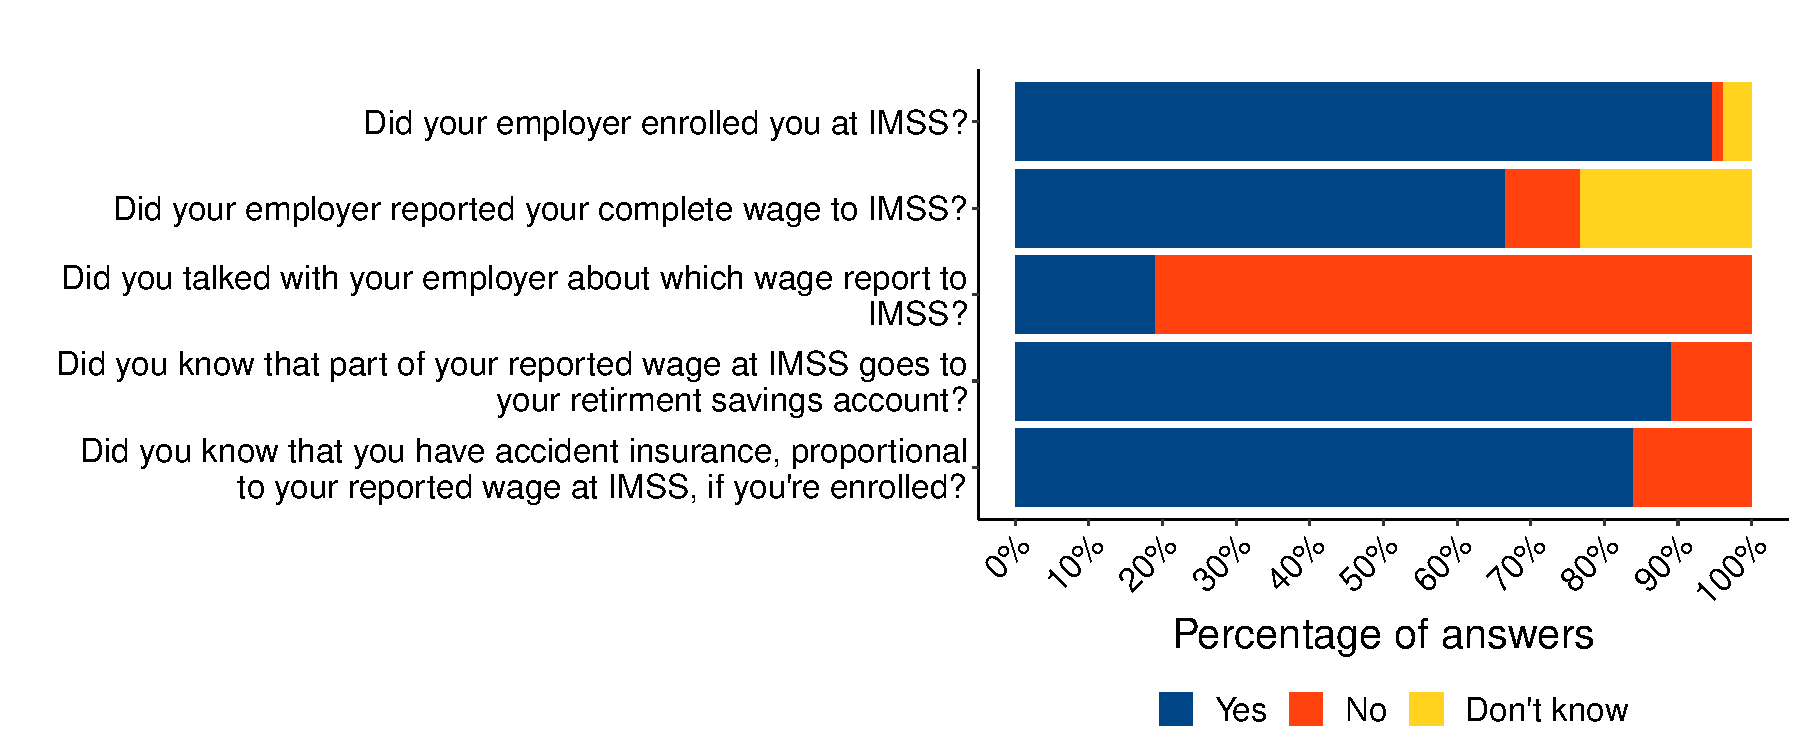
\includegraphics[width=\textwidth]{04_Figures/worker_survey/hist_knowledge_register_survey.pdf}
\end{figure}
\scriptsize{\textit{Notes}: This figure shows answers to questions about IMSS and wage reporting from the worker survey. \textit{Sample:} \hl{num survey answers} answers from a survey conducted via email to workers enrolled at IMSS during August 2021. Questions 1-2, about the worker's employer, included the option "I don't know". Questions 3-5 ask about the worker's actions or knowledge didn't include the option "I don't know".  This figure is referenced in \hyperref[sec:context]{Section} \ref{sec:context}.}

\clearpage

\subsection{Event studies}

\begin{figure}[H]
    \centering
    \caption{Event studies - RPCI effect on enrollment and wages \label{fig:event_study_rpci}}
    
    \begin{subfigure}{0.49\textwidth}
    \caption{Effect on being enrolled}
    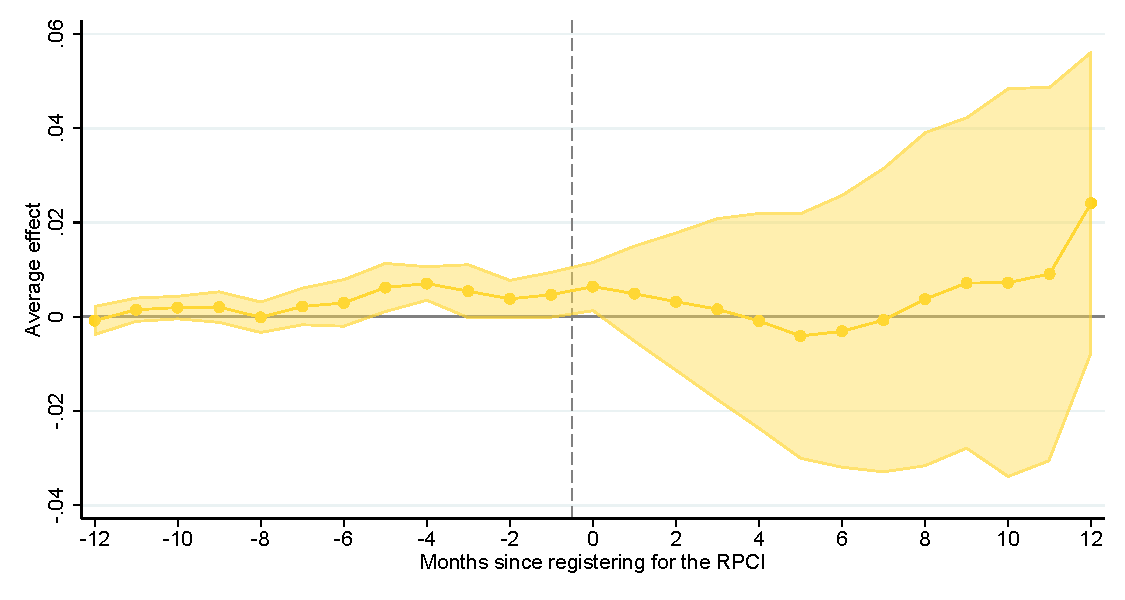
\includegraphics[width=\textwidth]{04_Figures/muestra_10porciento/event_study_alta_dcdh_connected.pdf}
    \end{subfigure}
    \begin{subfigure}{0.49\textwidth}
    \caption{Effect on formal wage}
    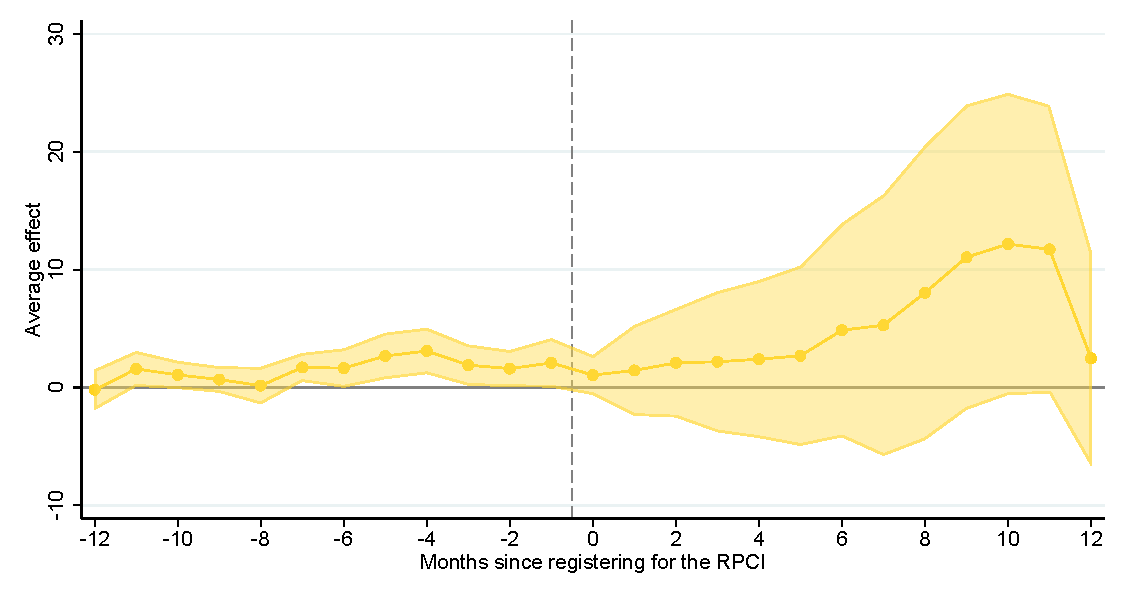
\includegraphics[width=\textwidth]{04_Figures/muestra_10porciento/event_study_sal_formal_dcdh_connected.pdf}
    \end{subfigure}
    
    \begin{subfigure}{0.49\textwidth}
    \caption{Effect on wage$^\dagger$}
    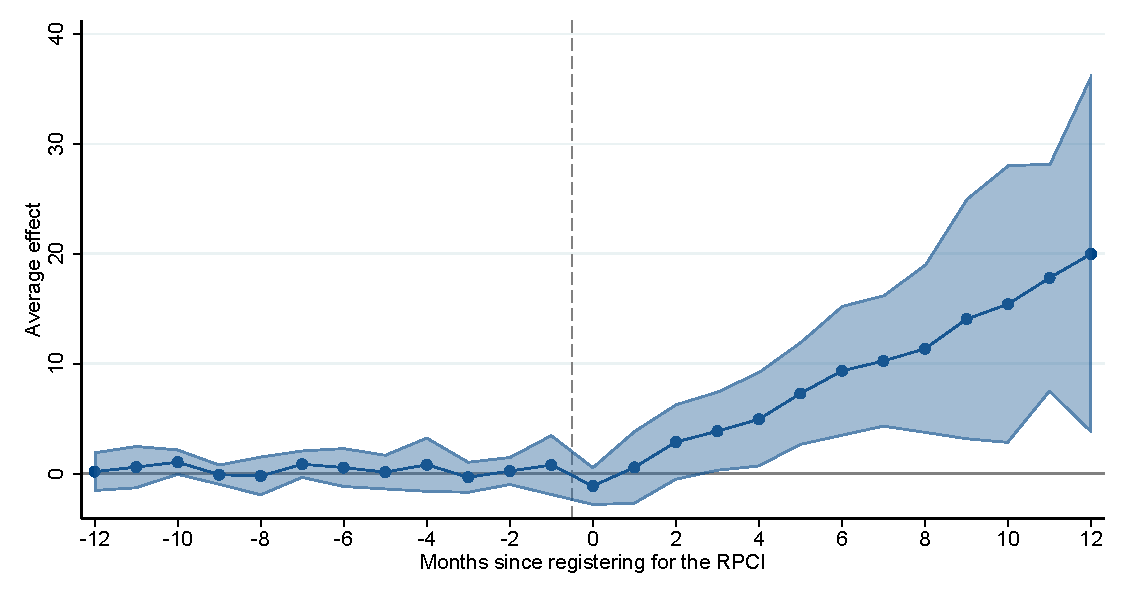
\includegraphics[width=\textwidth]{04_Figures/muestra_10porciento/event_study_sal_cierre_dcdh_connected.pdf}
    \end{subfigure}
    
    %\textit{Do file: event_study_rpci.do}
\end{figure}
\scriptsize{\textit{Notes}: This figure shows the event studies for the effect of registering to the RPCI on enrollment and the worker's wage. \textit{Sample:} Panel data for a random sample of the workers enrolled at the Mexican Institute of Social Security (IMSS) during January 2021 (before the RPCI launch). \textit{Enrolled} is a dummy variable where 1 means worker $i$ was enrolled at IMSS during period $t$. $\dagger$ \textit{Formal Wage}, \textit{Wage} and \textit{Log Wage} are the registered wage for worker $i$ during period $t$, the difference is \textit{Formal Wage} is 0 when the worker isn't enrolled, while \textit{Wage} and \textit{Log Wage} are missing when the worker isn't enrolled. The TWFE event studies use the extended TWFE specification following \cite{wooldridge2021two}, $y_{it} = \gamma_{i} + \theta_{t}+ \beta RPCI_{it} + \mathrm{X_i}\cdot\Pi_t +\epsilon_{it}$, where $\gamma_{i}$ are dummies for each worker id, $\theta_{t}$ are dummies for each monthly period, and $RPCI_{it}$ are dummies where 1 means that the worker registered for the RPCI during that month or previous month. Regressions include fixed effects on linear trends, by interacting a set of dummies for each quarterly period ($\Pi_t)$ with dummies on worker's baseline characteristics and cohort ($\mathrm{X_i}$): age group, firm industry, state, wage decile, and cohort. Robust standard errors clustered by worker id. TWFE event studies may be biased in the presence of heterogeneous treatment effects across cohorts. To address this, the second event study follows the specification in \cite{de2020two}, with robust dynamic for possible heterogeneous effects across treatment cohorts. This figure is referenced in \hyperref[subsec:workers]{Section} \ref{subsec:workers}.}


\begin{figure}[H]
    \caption{RPCI registers by month}
    \label{hist_download}
    \begin{center}
    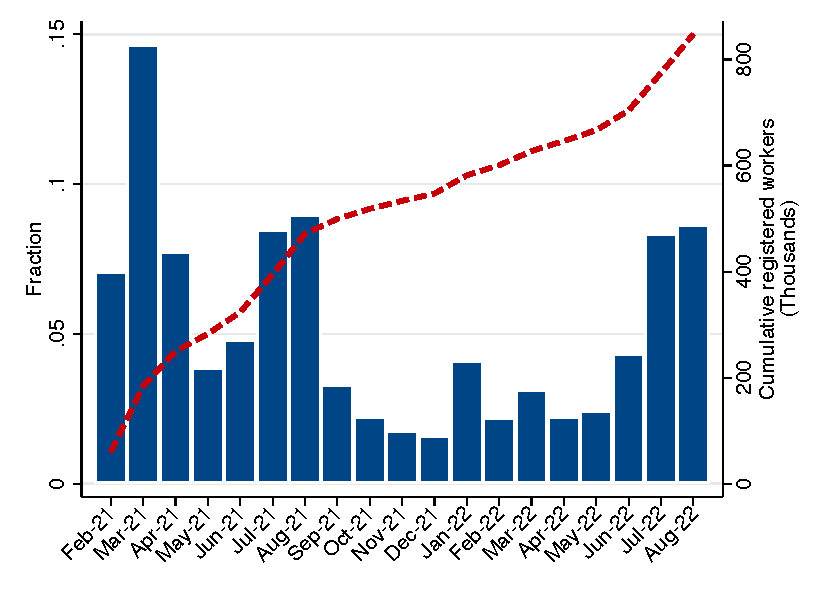
\includegraphics[width=0.75\textwidth]{04_Figures/muestra_1porciento/hist_download_month.pdf}
    \end{center}
\end{figure}
\scriptsize{
\noindent \textit{Sample:} 10\% of the workers registered at the Mexican Institute of Social Security (IMSS) between January 2020 and August 2022. The right y-axis measures the fraction of workers who registered for the RPCI during each month from the total workers who registered for the RPCI in the sample. The left y-axis measures the cumulative number of workers who registered for the RPCI in the sample.
}

\clearpage

\begin{figure}[H]
    \caption{Event studies - RPCI effect}
    \label{event_study}
    \begin{center}
    
    \begin{subfigure}{0.49\textwidth}
    \caption{Effect on wage}
    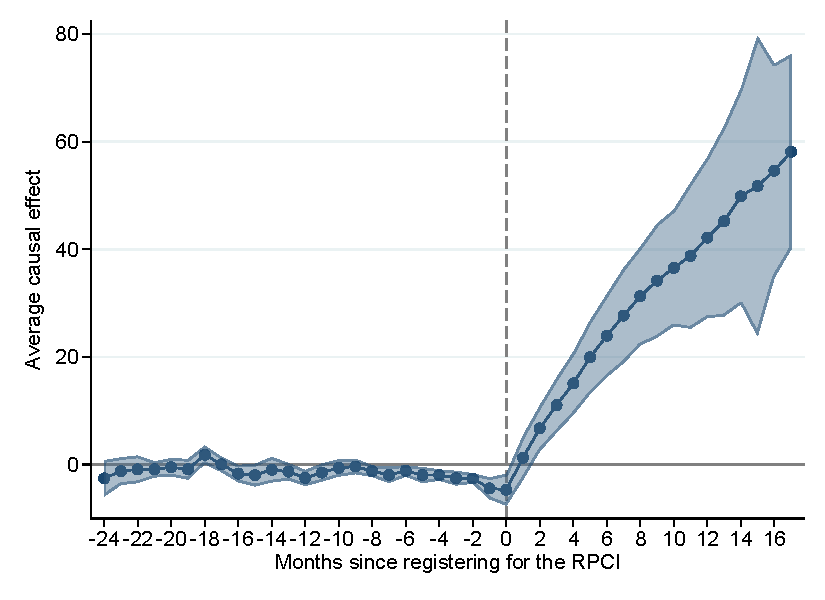
\includegraphics[width=\textwidth]{04_Figures/muestra_10porciento/event_study_sal_cierre_chaisemartin.pdf}
    \end{subfigure}
    \begin{subfigure}{0.49\textwidth}
    \caption{Effect on log wage}
    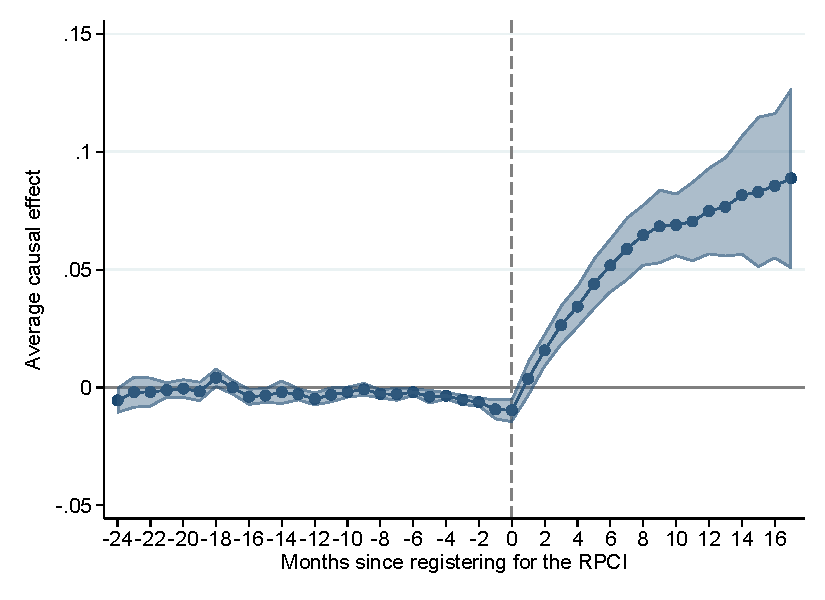
\includegraphics[width=\textwidth]{04_Figures/muestra_10porciento/event_study_log_sal_cierre_chaisemartin.pdf}
    \end{subfigure}
    
    \begin{subfigure}{0.49\textwidth}
    \caption{Effect on being enrolled}
    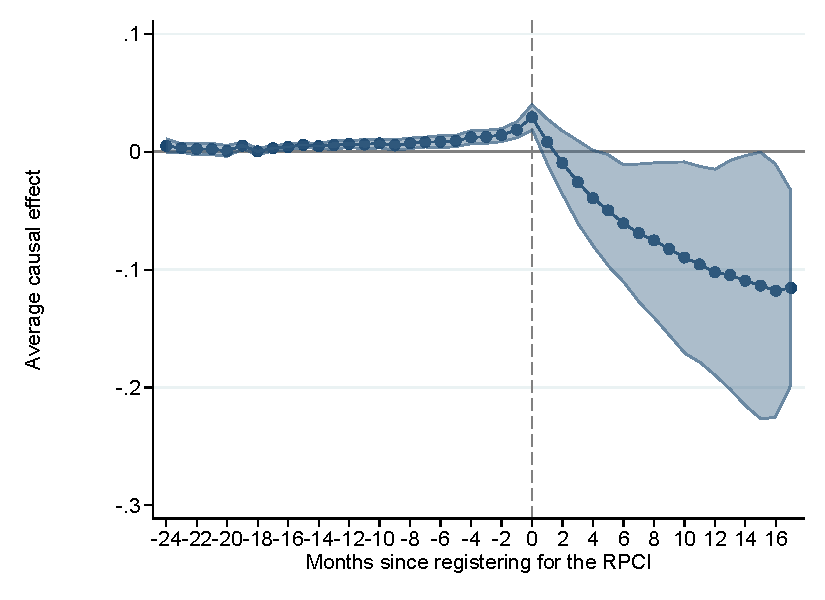
\includegraphics[width=\textwidth]{04_Figures/muestra_10porciento/event_study_alta_chaisemartin.pdf}
    \end{subfigure}
    \begin{subfigure}{0.49\textwidth}
    \caption{Effect on enrollment}
    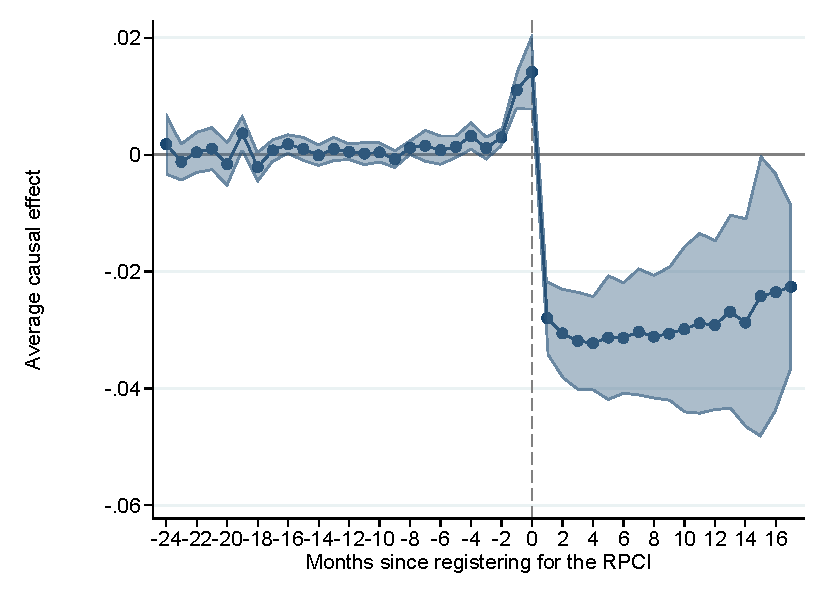
\includegraphics[width=\textwidth]{04_Figures/muestra_10porciento/event_study_alta_cierre_chaisemartin.pdf}
    \end{subfigure}
    
    \begin{subfigure}{0.49\textwidth}
    \caption{Effect on discharge}
    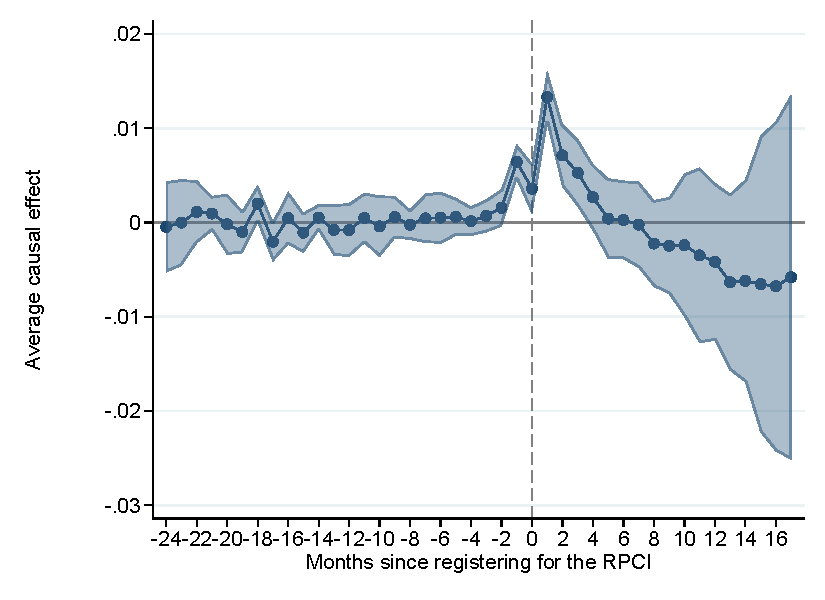
\includegraphics[width=\textwidth]{04_Figures/muestra_10porciento/event_study_baja_cierre_chaisemartin.pdf}
    \end{subfigure}
    \begin{subfigure}{0.49\textwidth}
    \caption{Effect on permanent discharge}
    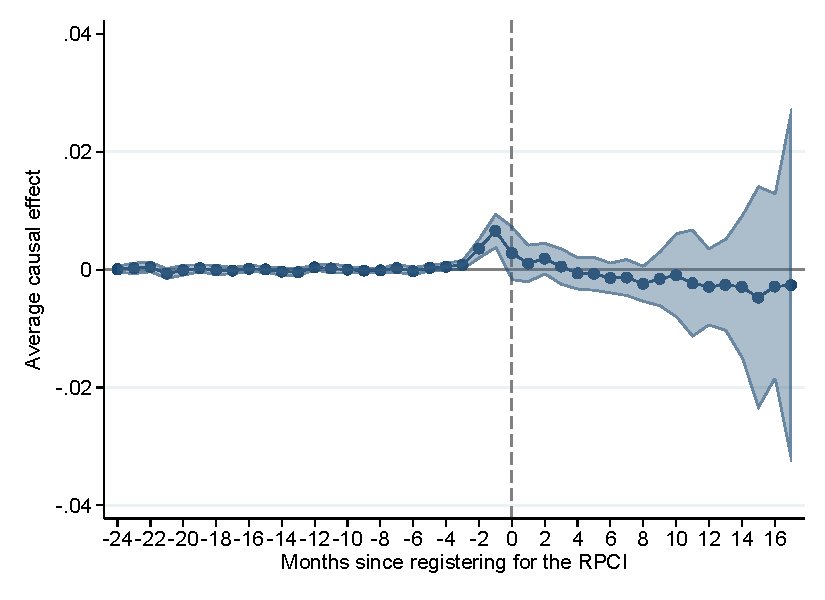
\includegraphics[width=\textwidth]{04_Figures/muestra_10porciento/event_study_baja_permanente_chaisemartin.pdf}
    \end{subfigure}
    
    %\textit{Do file: did_multiplegt_rpci.do}
    \end{center}
\end{figure}
\scriptsize{
\noindent \textit{Sample:} 10\% of the workers registered at the Mexican Institute of Social Security (IMSS) between January 2020 and August 2022. The graphs use the estimators proposed by Chaisemartin and D'Haultfoeuille to prevent posible negative weights in the Difference in Differences estimators.
}

\clearpage

\begin{figure}[H]
    \ContinuedFloat
    \caption{(Continued) Event studies - RPCI effect}
    \label{event_study_cont}
    \begin{center}
    
    \begin{subfigure}{0.49\textwidth}
    \caption{Effect on wage change}
    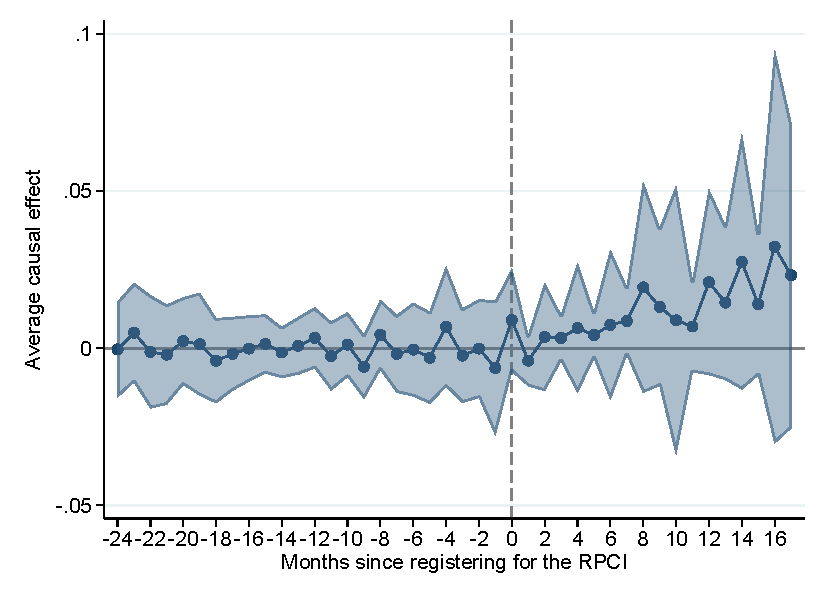
\includegraphics[width=\textwidth]{04_Figures/muestra_10porciento/event_study_sal_diff_chaisemartin.pdf}
    \end{subfigure}
    \begin{subfigure}{0.49\textwidth}
    \caption{Effect on job change}
    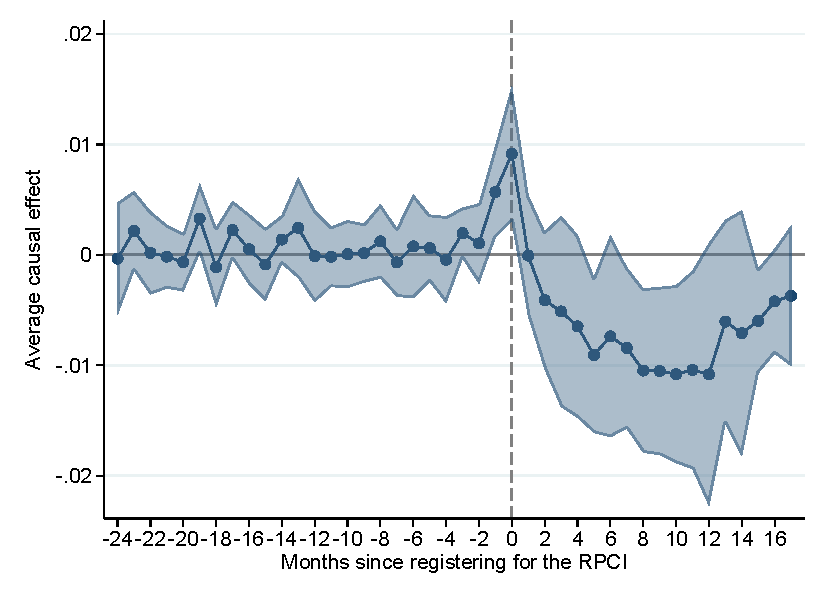
\includegraphics[width=\textwidth]{04_Figures/muestra_10porciento/event_study_cambio_cierre_chaisemartin.pdf}
    \end{subfigure}

    %\textit{Do file: did_multiplegt_rpci.do}
    \end{center}
\end{figure}
\scriptsize{
\noindent \textit{Sample:} 10\% of the workers registered at the Mexican Institute of Social Security (IMSS) between January 2020 and August 2022. The graphs use the estimators proposed by Chaisemartin and D'Haultfoeuille to prevent posible negative weights in the Difference in Differences estimators.
}

\clearpage

\begin{figure}[H]
    \caption{Workers by the number of months observed after registering for the RPCI}
    \label{hist_time_since_treated}
    \begin{center}
    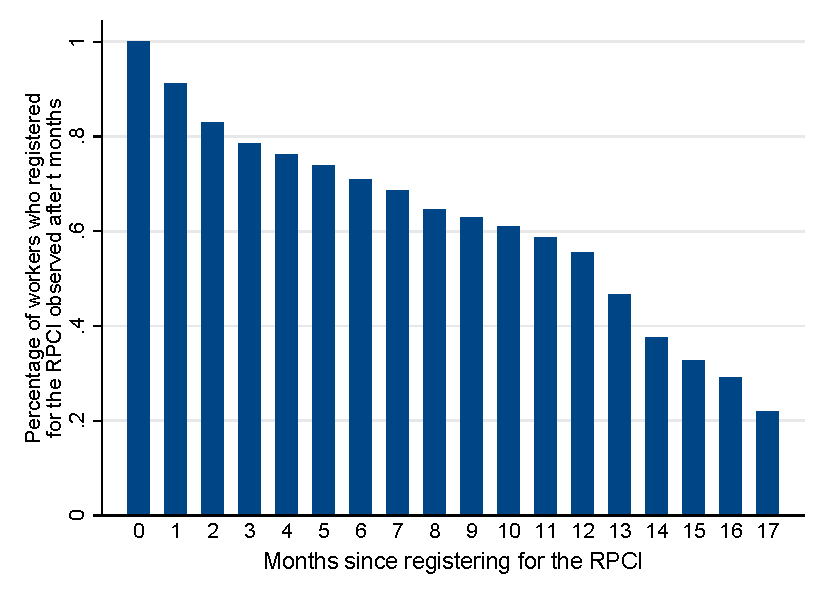
\includegraphics[width=0.5\textwidth]{04_Figures/muestra_10porciento/hist_time_since_treated.pdf}
    \end{center}
\end{figure}
\scriptsize{
\noindent \textit{Sample:} 10\% of the workers registered at the Mexican Institute of Social Security (IMSS) between January 2020 and August 2022. Not all workers registered for the RPCI at the same time, so not all workers are observed the same number of months after registering for the RPCI in the sample. The y-axis measures the percentage of workers observed $t$ months after registering for the RPCI from the total number of workers who registered for the RPCI.
}

\clearpage

\begin{figure}[H]
    \caption{Percentage of workers having the same wage after the RPCI}
    \label{hist_wage_time_since_treated}
    \begin{center}
    
    \begin{subfigure}{0.49\textwidth}
    \caption{Treatment: after registering for the RPCI}
    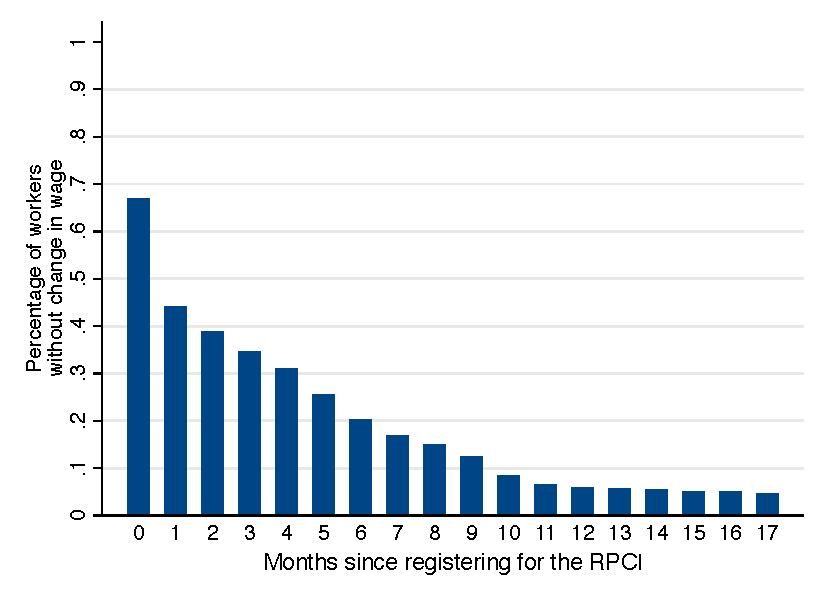
\includegraphics[width=\textwidth]{04_Figures/muestra_1porciento/hist_wage_time_since_treated_treat.pdf}
    \end{subfigure}
    \begin{subfigure}{0.49\textwidth}
    \caption{Control: after the RPCI launch}
    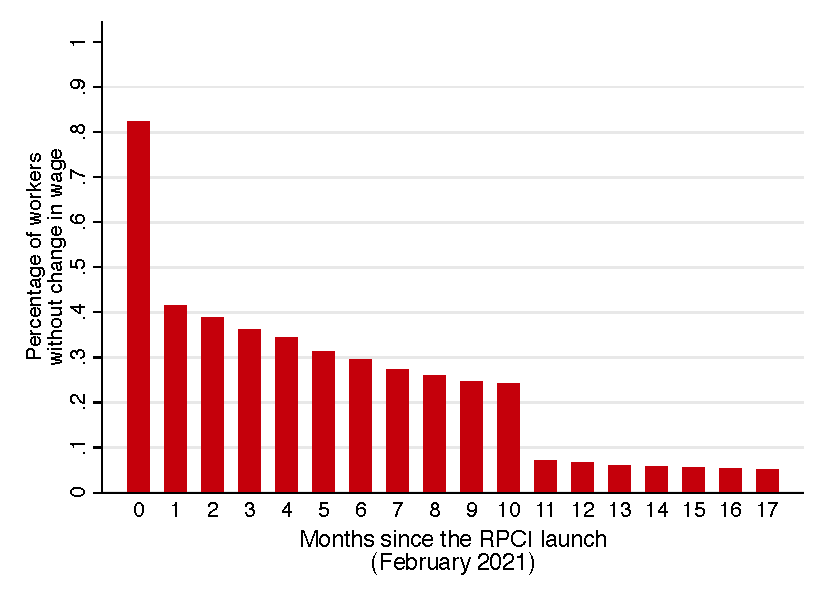
\includegraphics[width=\textwidth]{04_Figures/muestra_1porciento/hist_wage_time_since_treated_control.pdf}
    \end{subfigure}
    
    %\textit{Do file: hist_wage_time_since_treated.do}
    \end{center}
\end{figure}
\scriptsize{
\noindent This figures plot the percentage of workers that have the same wage after $t$ months. \textit{Sample:} 1\% of the workers registered at the Mexican Institute of Social Security (IMSS) between January 2020 and August 2022. For the treatment group, compares the wage the worker had one month before registering for the RPCI with the wage after $t$ months of the register. For the control group, compares the wage of January 2021, the month before the RPCI launch, with the wage $t$ months after. The y-axis measures the percentage of workers observed $t$ months with the same wage as in $t = -1$.
\todo[inline]{Marco: I repeated this figure with the matched data, since the control figure has clear seasonality. I matched on baseline characteristics and attributed to each control worker the register date of their treated match.}
}

\clearpage

\begin{figure}[H]
    \caption{Percentage of workers having the same wage after the RPCI - Matched data}
    \label{hist_wage_time_since_treated_matched}
    \begin{center}
    
    \begin{subfigure}{0.49\textwidth}
    \caption{Treatment: after registering for the RPCI}
    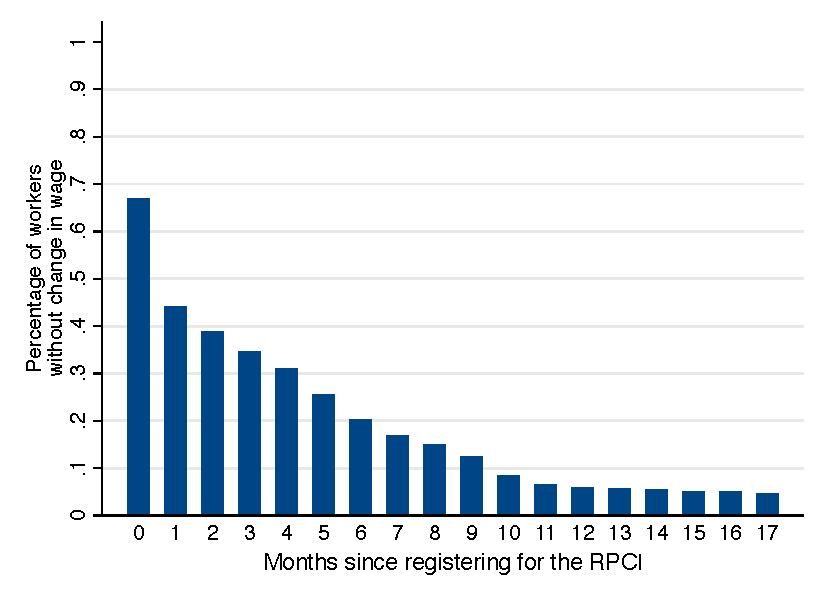
\includegraphics[width=\textwidth]{04_Figures/muestra_1porciento/hist_wage_time_since_treated_treat.pdf}
    \end{subfigure}
    \begin{subfigure}{0.49\textwidth}
    \caption{Control: after registering for the RPCI}
    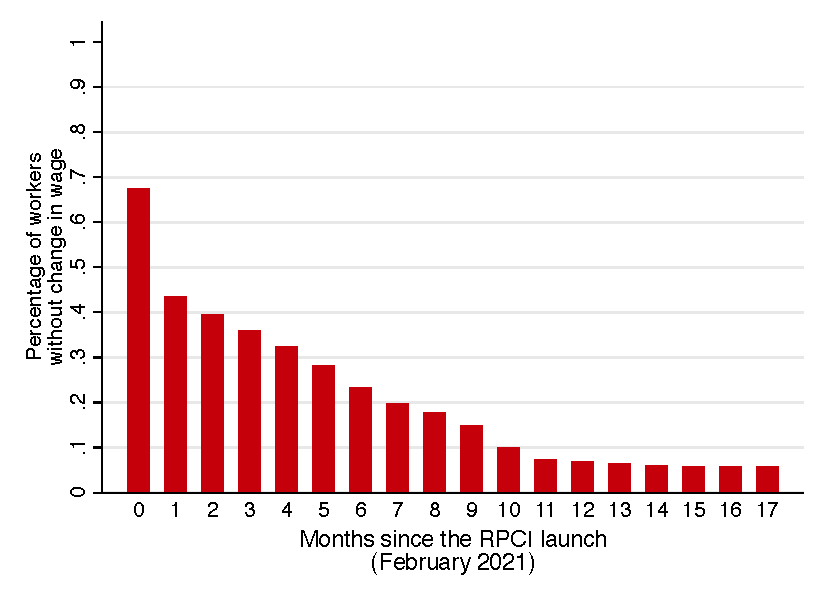
\includegraphics[width=\textwidth]{04_Figures/muestra_1porciento/hist_wage_time_since_treated_control_matched.pdf}
    \end{subfigure}
    
    \begin{subfigure}{0.49\textwidth}
    \caption{Difference (pp.) of the percentage of workers having the same wage by treatment status}
    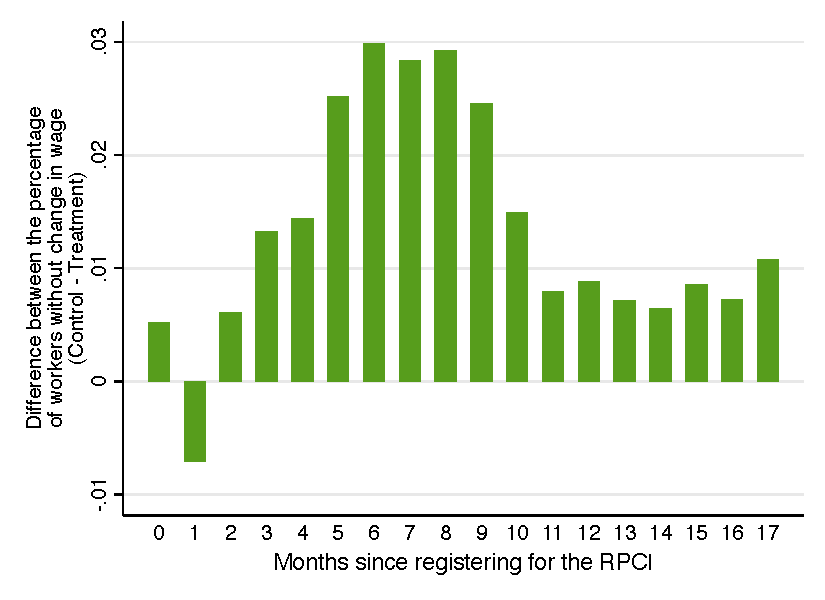
\includegraphics[width=\textwidth]{04_Figures/muestra_1porciento/hist_wage_time_since_treated_diff_matched.pdf}
    \end{subfigure}
    
    %\textit{Do file: hist_wage_time_since_treated.do}
    \end{center}
\end{figure}
\scriptsize{
\noindent This figure explores over time if workers that registered for the RPCI change their wages faster than workers who didn't register for the RPCI. The figures plot the percentage of workers that have the same wage after $t$ months. The workers that didn't register for the RPCI get the register date from the matched worker that did register for the RPCI, using nearest neighbor matching on the worker's baseline characteristics. \textit{Sample:} 1\% of the workers registered at the Mexican Institute of Social Security (IMSS) between January 2020 and August 2022. For the treatment group, compares the wage the worker had one month before registering for the RPCI with the wage after $t$ months of the register. For the control group, compares the wage the worker had one month before their matched treated worker registered for the RPCI, with the wage after $t$ months of the register. The y-axis measures the percentage of workers observed $t$ months with the same wage as in $t = -1$. Figure (c) present the difference between the bars in figures (b) and (a).
}


\clearpage

\begin{figure}[H]
    \caption{RPCI effect by cohort}
    \label{twfe_beta_cohort}
    \begin{center}
    
    \begin{subfigure}{0.49\textwidth}
    \caption{Effect on wage}
    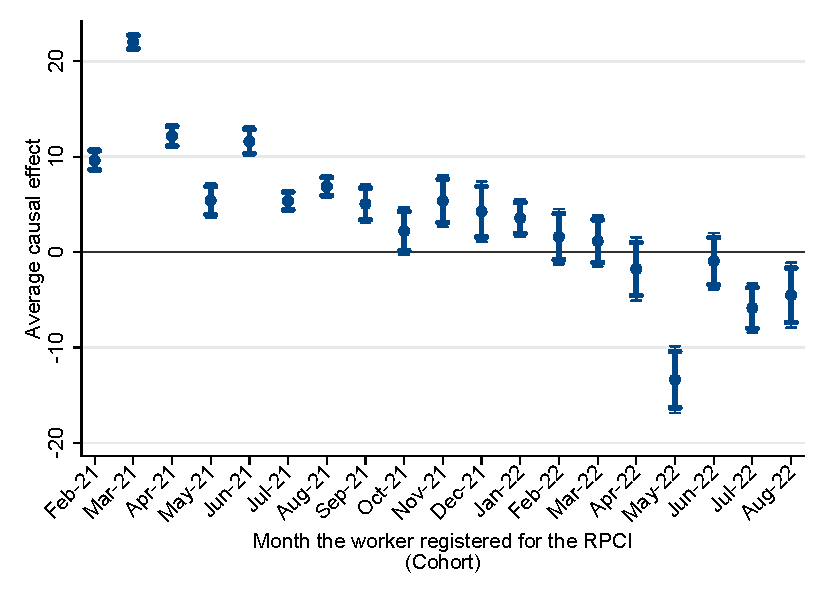
\includegraphics[width=\textwidth]{04_Figures/muestra_10porciento/twfe_beta_cohort_sal_cierre.pdf}
    \end{subfigure}
    \begin{subfigure}{0.49\textwidth}
    \caption{Effect on log wage}
    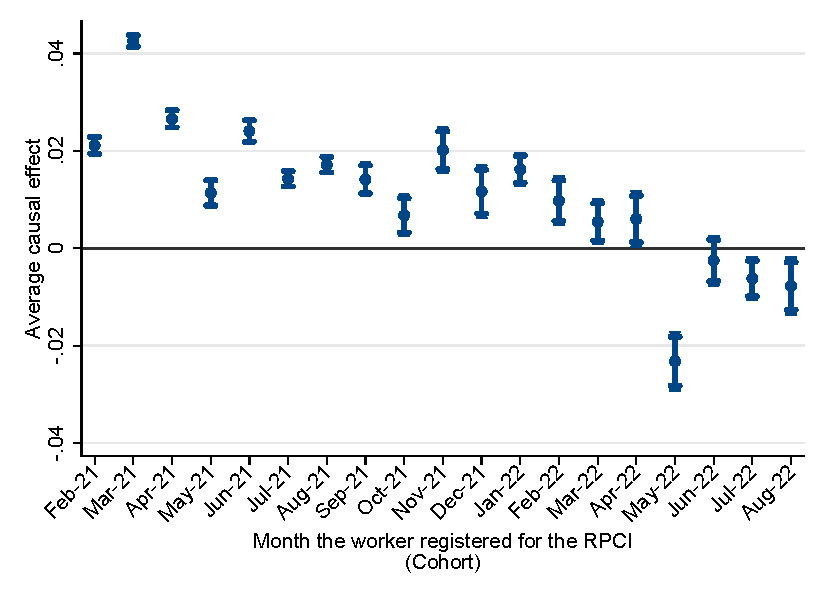
\includegraphics[width=\textwidth]{04_Figures/muestra_10porciento/twfe_beta_cohort_log_sal_cierre.pdf}
    \end{subfigure}

    \begin{subfigure}{0.49\textwidth}
    \caption{Effect on wage}
    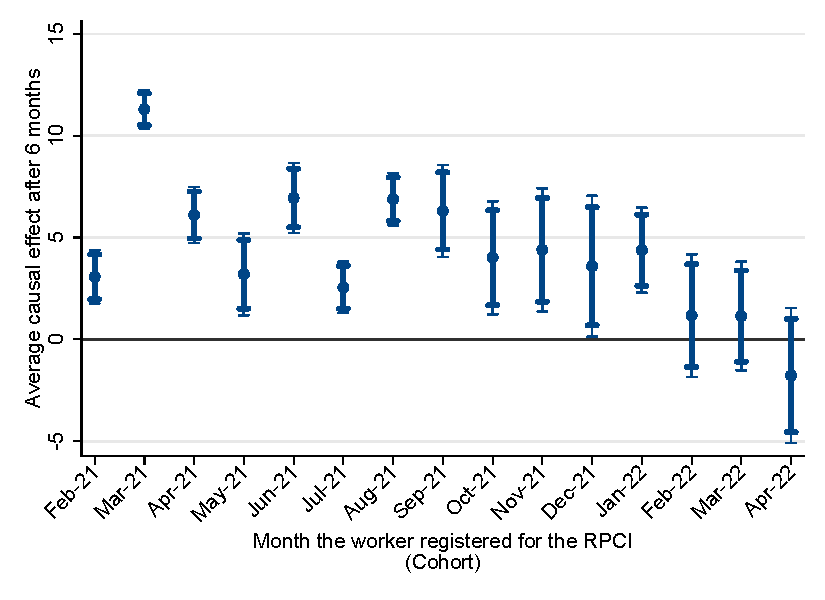
\includegraphics[width=\textwidth]{04_Figures/muestra_10porciento/twfe_beta_cohort_sal_cierre_6m.pdf}
    \end{subfigure}
    \begin{subfigure}{0.49\textwidth}
    \caption{Effect on log wage}
    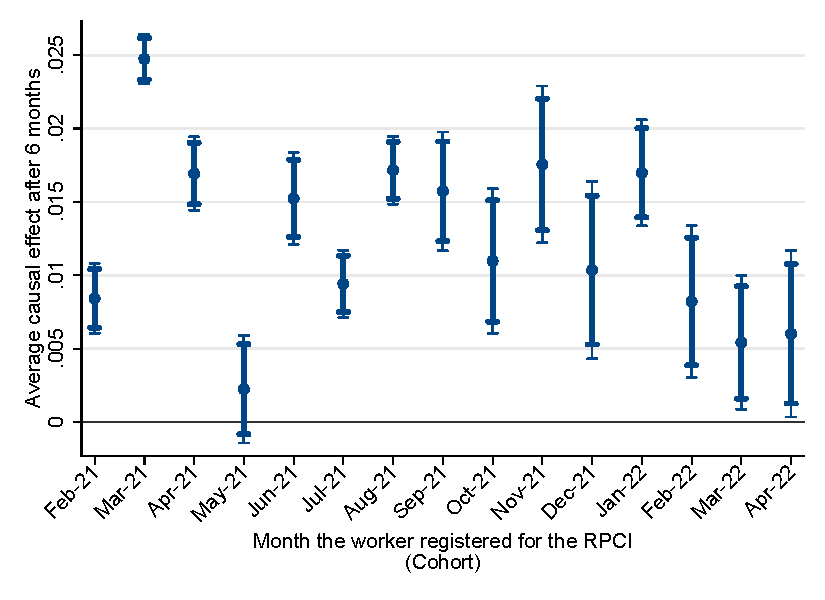
\includegraphics[width=\textwidth]{04_Figures/muestra_10porciento/twfe_beta_cohort_log_sal_cierre_6m.pdf}
    \end{subfigure}
    
    %\textit{Do file: twfe_beta_cohort_rpci.do}
    \end{center}
\end{figure}
\scriptsize{
\noindent \textit{Sample:} 10\% of the workers registered at the Mexican Institute of Social Security (IMSS) between January 2020 and August 2022. Each point in the graph corresponds to the estimated regression coefficient where the sample conditions the treatment group by the cohort of register for the RPCI. All regressions have the same control group, meaning all samples include the workers who never registered for the RPCI. Regressions use the TWFE specification $y_{it} = \gamma_{i} + \theta_{t}+ \beta RPCI_{it} +\epsilon_{it}$, where $\gamma_{i}$ are dummies for each worker id, $\theta_{t}$ are dummies for each monthly period, and $RPCI_{it}$ are dummies where 1 means that the worker registered for the RPCI during that month or previous month, and include dummies for each state and dummies for each wage decile of the wage distribution during 2020, both interacted with dummies for each quarterly period. 
}
\todo[inline]{Make this figure again, but observing only 6 months after for all cohorts. This graph could reflect that RPCI takes time to happen.}

\clearpage

\begin{figure}[H]
    \caption{Event studies - RPCI effect on wage by cohort}
    \label{event_study_cohort}
    \begin{center}
    
    \begin{subfigure}{0.49\textwidth}
    \caption{Early adopters}
    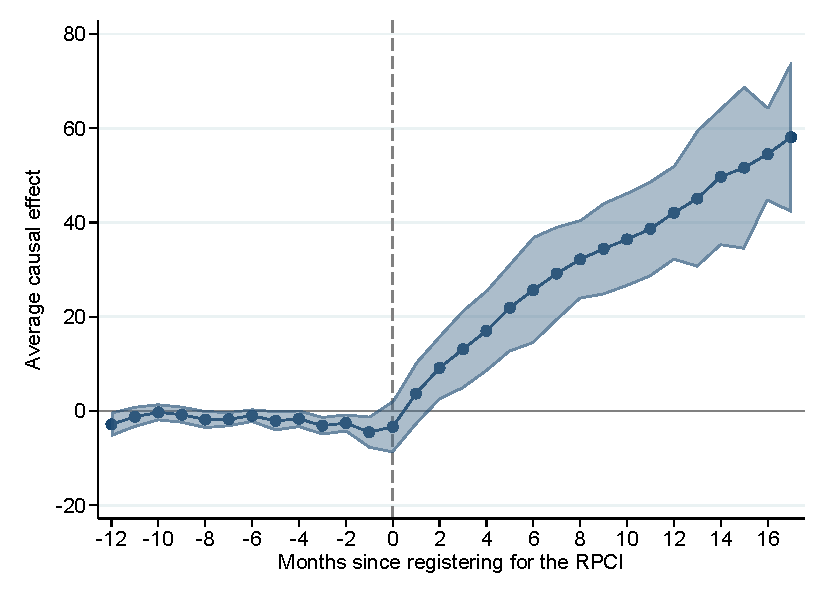
\includegraphics[width=\textwidth]{04_Figures/muestra_10porciento/event_study_sal_cierre_chaisemartin_adopters_early.pdf}
    \end{subfigure}
    \begin{subfigure}{0.49\textwidth}
    \caption{Late adopters}
    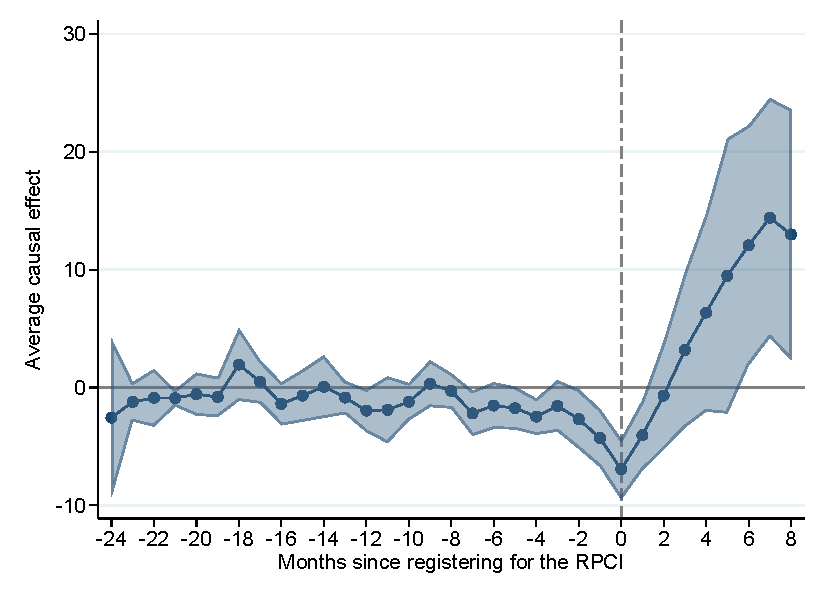
\includegraphics[width=\textwidth]{04_Figures/muestra_10porciento/event_study_sal_cierre_chaisemartin_adopters_late.pdf}
    \end{subfigure}
    
    \begin{subfigure}{0.49\textwidth}
    \caption{Early adopters using late adopters as control}
    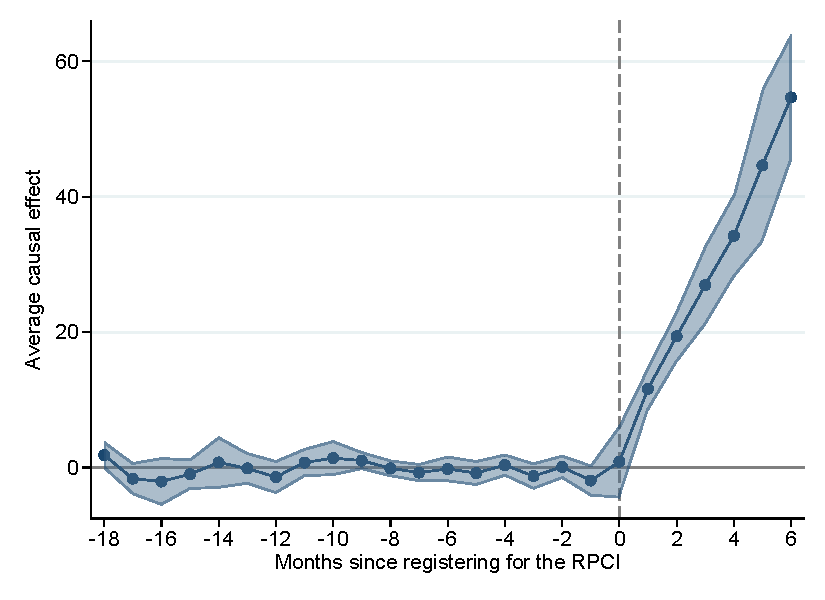
\includegraphics[width=\textwidth]{04_Figures/muestra_10porciento/event_study_sal_cierre_chaisemartin_adopters_early_late.pdf}
    \end{subfigure}
    
    %\textit{Do file: did_multiplegt_heterogeneity_rpci.do}
    \end{center}
\end{figure}
\scriptsize{
\noindent \textit{Sample:} 10\% of the workers registered at the Mexican Institute of Social Security (IMSS) between January 2020 and August 2022. The graphs use the estimators proposed by Chaisemartin and D'Haultfoeuille to prevent posible negative weights in the Difference in Differences estimators. Each subfigure conditions the treatment group by the cohort of register for the RPCI. Subfigure (a) conditions the treatment group to early adopters, meaning the workers who registered for the RPCI during the first nine months after the RPCI launch (February 2021 to October 2021). Subfigure (b) conditions the treatment group to late adopters, meaning the workers who registered for the RPCI during the next nine months (November 2021 to August 2022). Both subfigures have the same control group, meaning the workers who never registered for the RPCI. Subfigure (c) conditions the treatment group to early adopters and uses late adopters as control group.
}

\clearpage

\begin{figure}[H]
    \caption{Event studies - RPCI effect on wage by worker characteristics}
    \label{event_study_wage_worker_characteristics}
    \begin{center}
    
    \begin{subfigure}{0.49\textwidth}
    \caption{Men}
    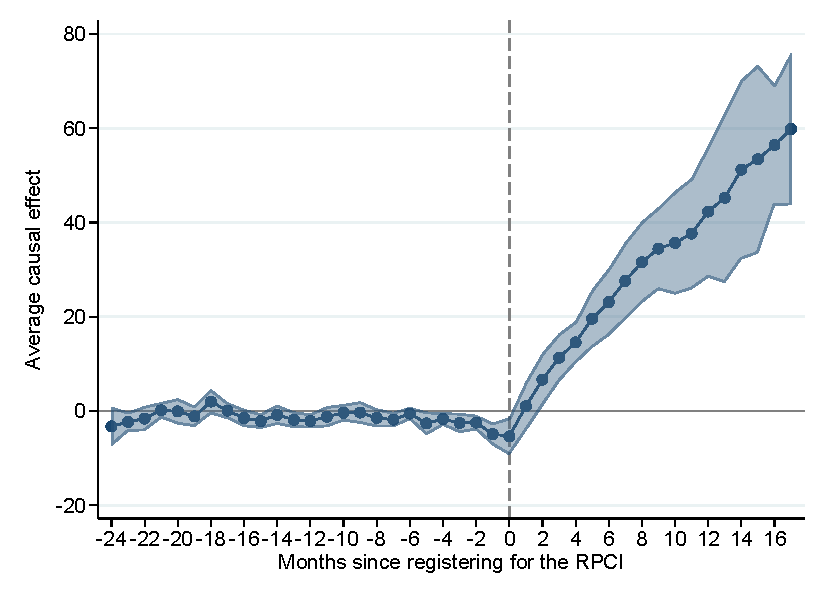
\includegraphics[width=\textwidth]{04_Figures/muestra_10porciento/event_study_sal_cierre_chaisemartin_sexo_0.pdf}
    \end{subfigure}
    \begin{subfigure}{0.49\textwidth}
    \caption{Woman}
    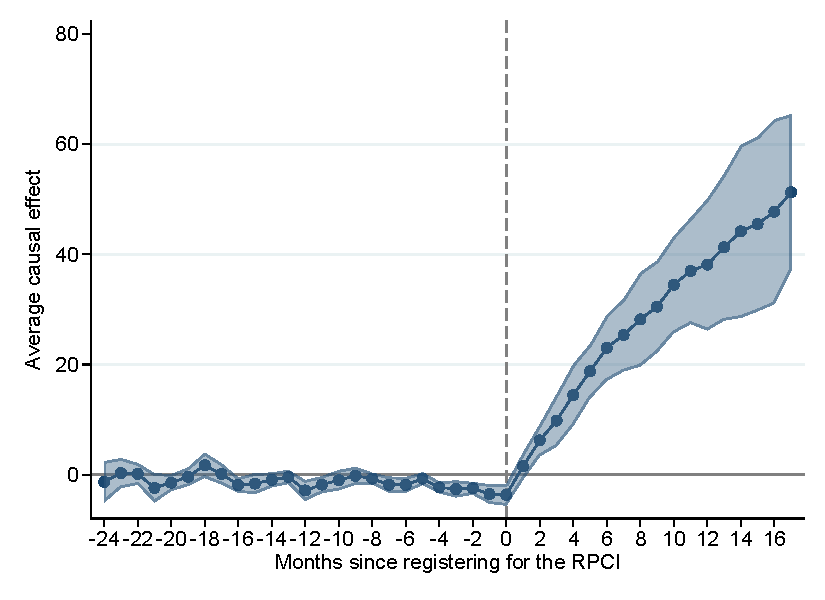
\includegraphics[width=\textwidth]{04_Figures/muestra_10porciento/event_study_sal_cierre_chaisemartin_sexo_1.pdf}
    \end{subfigure}
    
    \begin{subfigure}{0.49\textwidth}
    \caption{Outsourcing}
    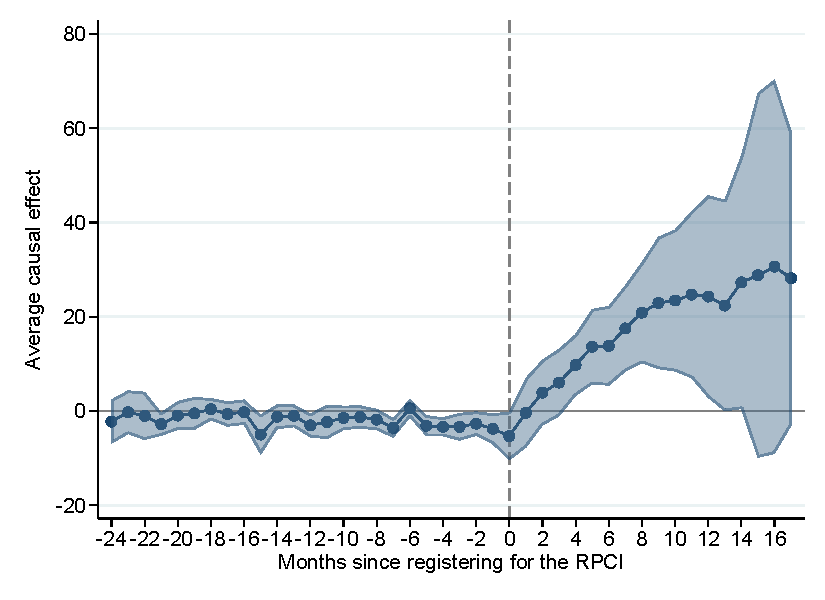
\includegraphics[width=\textwidth]{04_Figures/muestra_10porciento/event_study_sal_cierre_chaisemartin_outsourcing.pdf}
    \end{subfigure}
    \begin{subfigure}{0.49\textwidth}
    \caption{Temporary}
    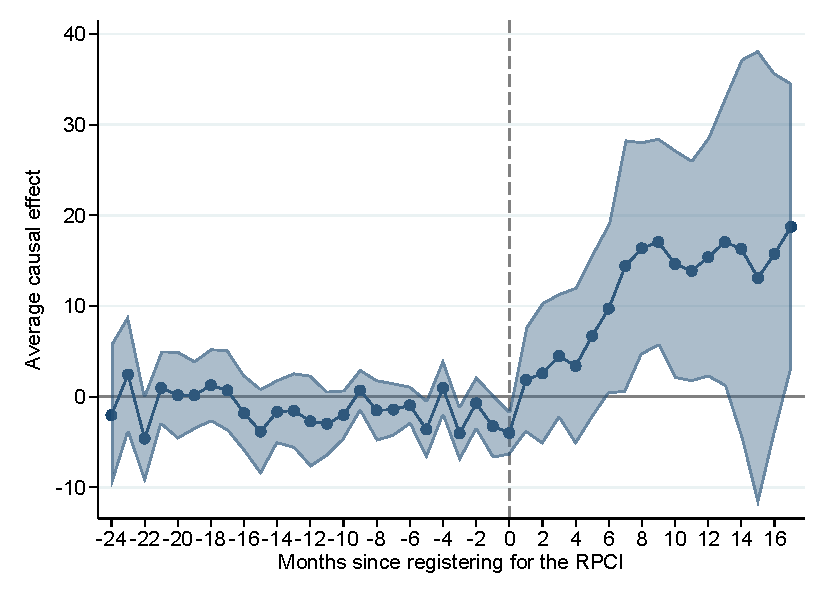
\includegraphics[width=\textwidth]{04_Figures/muestra_10porciento/event_study_sal_cierre_chaisemartin_eventual.pdf}
    \end{subfigure}
    
    %\textit{Do file: did_multiplegt_heterogeneity_rpci.do}
    \end{center}
\end{figure}
\scriptsize{
\noindent \textit{Sample:} 10\% of the workers registered at the Mexican Institute of Social Security (IMSS) between January 2020 and August 2022. The graphs use the estimators proposed by Chaisemartin and D'Haultfoeuille to prevent posible negative weights in the Difference in Differences estimators. Each subfigure conditions on a worker characteristics at baseline, during 2020, previous to the RPCI launch. Subfigures (a) and (b) condition on the worker gender. Subfigure (c) conditions on workers hired through outsourcing. Subfigure (d) conditions on temporary workers.
}

\clearpage

\begin{figure}[H]
    \caption{Event studies - RPCI effect on log wage by worker characteristics}
    \label{event_study_log_wage_worker_characteristics}
    \begin{center}
    
    \begin{subfigure}{0.49\textwidth}
    \caption{Men}
    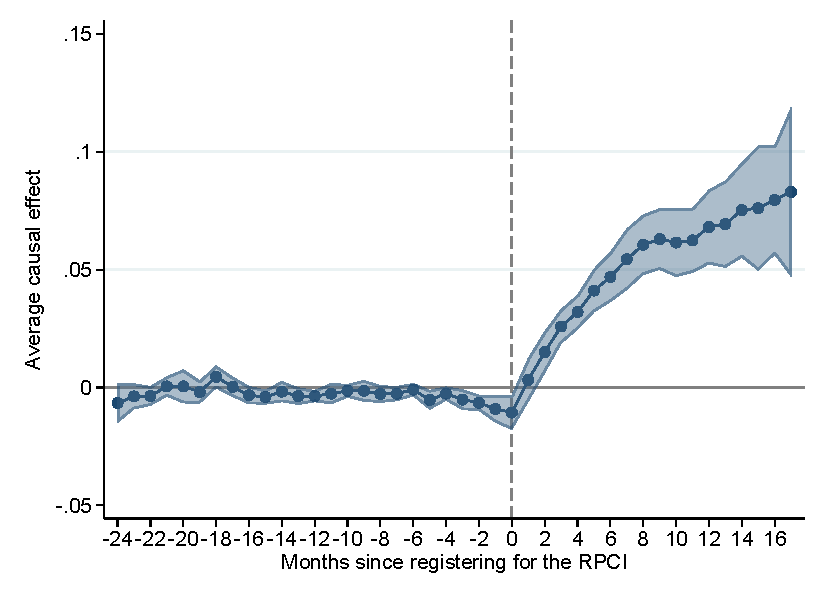
\includegraphics[width=\textwidth]{04_Figures/muestra_10porciento/event_study_log_sal_cierre_chaisemartin_sexo_0.pdf}
    \end{subfigure}
    \begin{subfigure}{0.49\textwidth}
    \caption{Woman}
    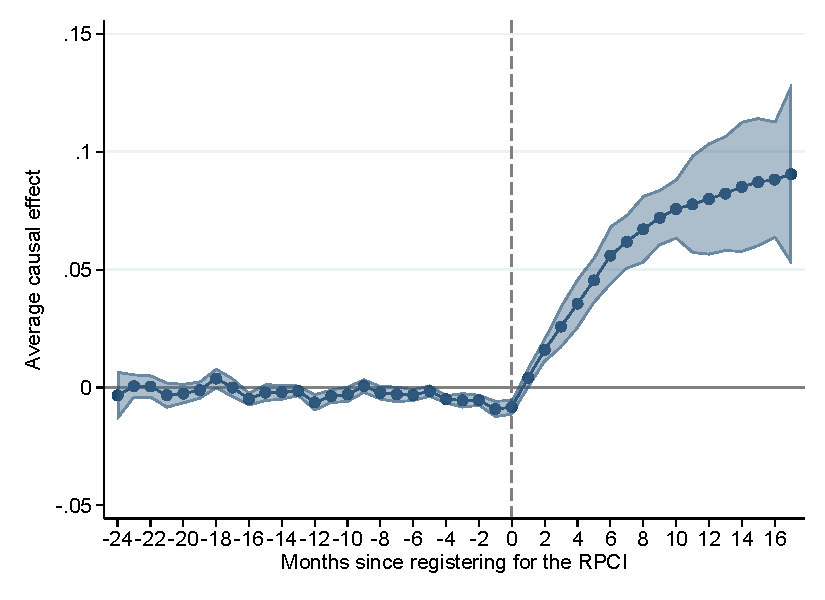
\includegraphics[width=\textwidth]{04_Figures/muestra_10porciento/event_study_log_sal_cierre_chaisemartin_sexo_1.pdf}
    \end{subfigure}
    
    \begin{subfigure}{0.49\textwidth}
    \caption{Outsourcing}
    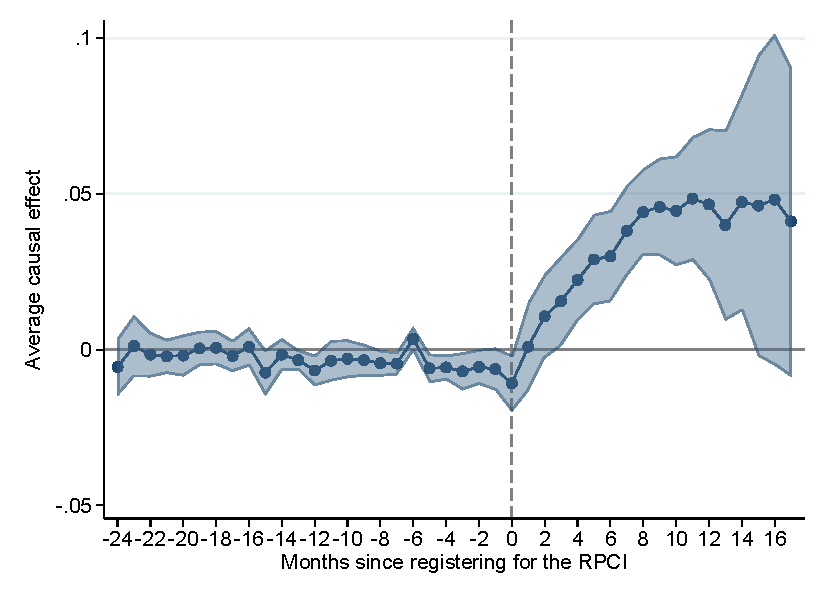
\includegraphics[width=\textwidth]{04_Figures/muestra_10porciento/event_study_log_sal_cierre_chaisemartin_outsourcing.pdf}
    \end{subfigure}
    \begin{subfigure}{0.49\textwidth}
    \caption{Temporary}
    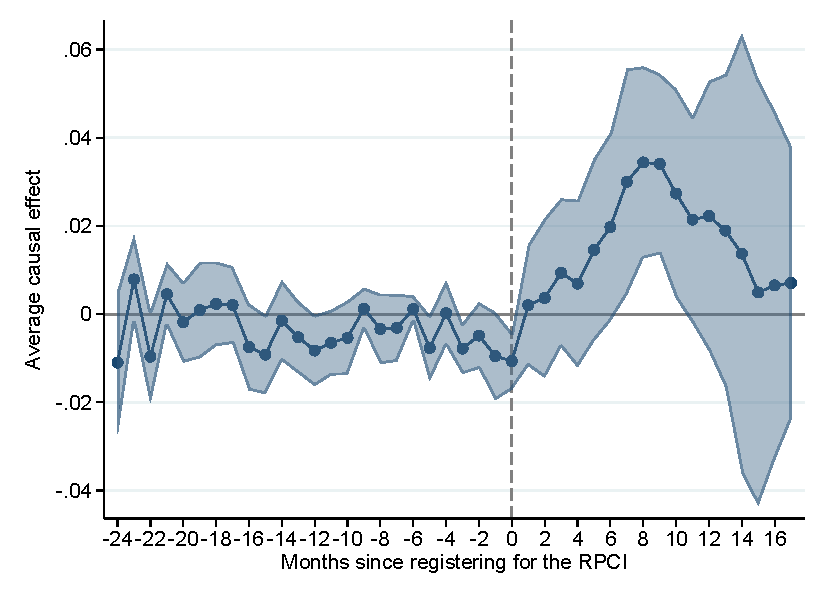
\includegraphics[width=\textwidth]{04_Figures/muestra_10porciento/event_study_log_sal_cierre_chaisemartin_eventual.pdf}
    \end{subfigure}
    
    %\textit{Do file: did_multiplegt_heterogeneity_rpci.do}
    \end{center}
\end{figure}
\scriptsize{
\noindent \textit{Sample:} 10\% of the workers registered at the Mexican Institute of Social Security (IMSS) between January 2020 and August 2022. The graphs use the estimators proposed by Chaisemartin and D'Haultfoeuille to prevent posible negative weights in the Difference in Differences estimators. Each subfigure conditions on a worker characteristics at baseline, during 2020, previous to the RPCI launch. Subfigures (a) and (b) condition on the worker gender. Subfigure (c) conditions on workers hired through outsourcing. Subfigure (d) conditions on temporary workers.
}

\clearpage

\begin{figure}[H]
    \caption{Event studies - RPCI effect on wage by firm characteristics}
    \label{event_study_wage_firm_characteristics}
    \begin{center}
    
    \begin{subfigure}{0.49\textwidth}
    \caption{Transformation Industry}
    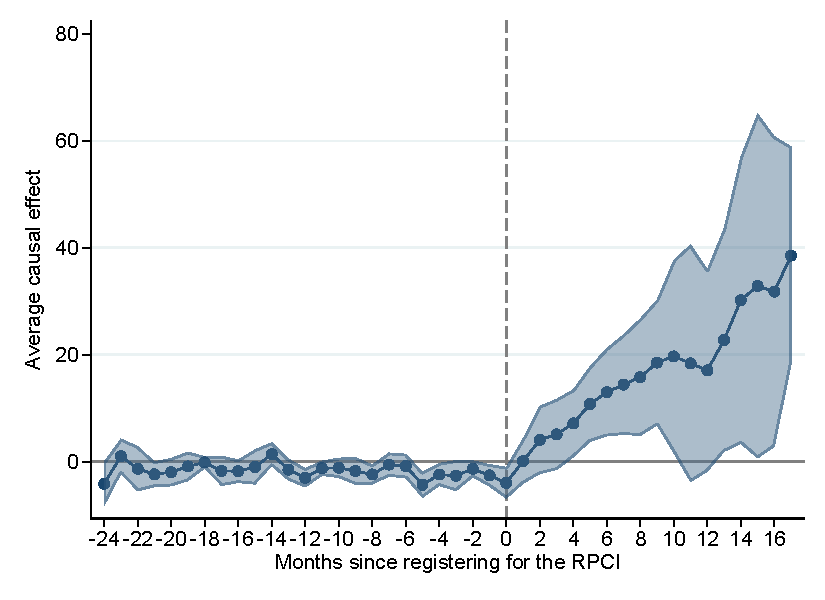
\includegraphics[width=\textwidth]{04_Figures/muestra_10porciento/event_study_sal_cierre_chaisemartin_div_final_3.pdf}
    \end{subfigure}
    \begin{subfigure}{0.49\textwidth}
    \caption{Construction Industry}
    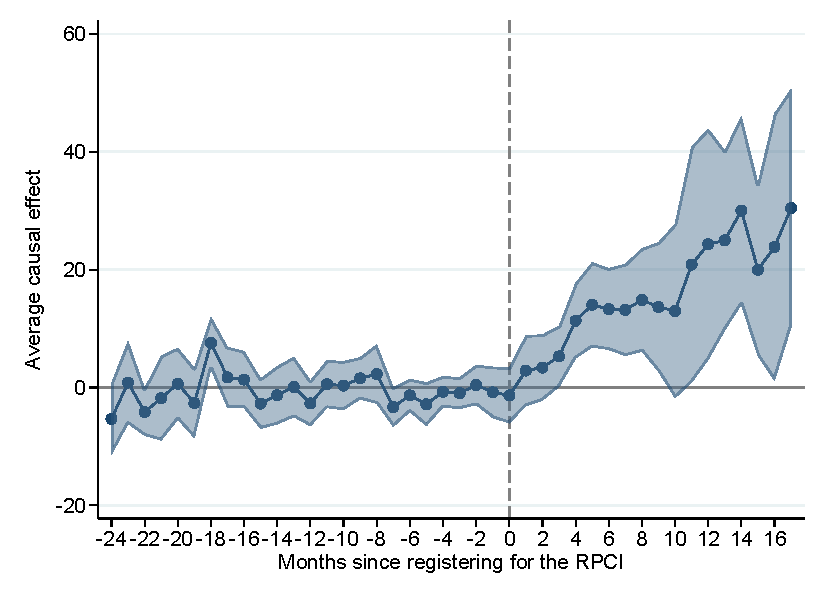
\includegraphics[width=\textwidth]{04_Figures/muestra_10porciento/event_study_sal_cierre_chaisemartin_div_final_4.pdf}
    \end{subfigure}
    
    \begin{subfigure}{0.49\textwidth}
    \caption{Commerce}
    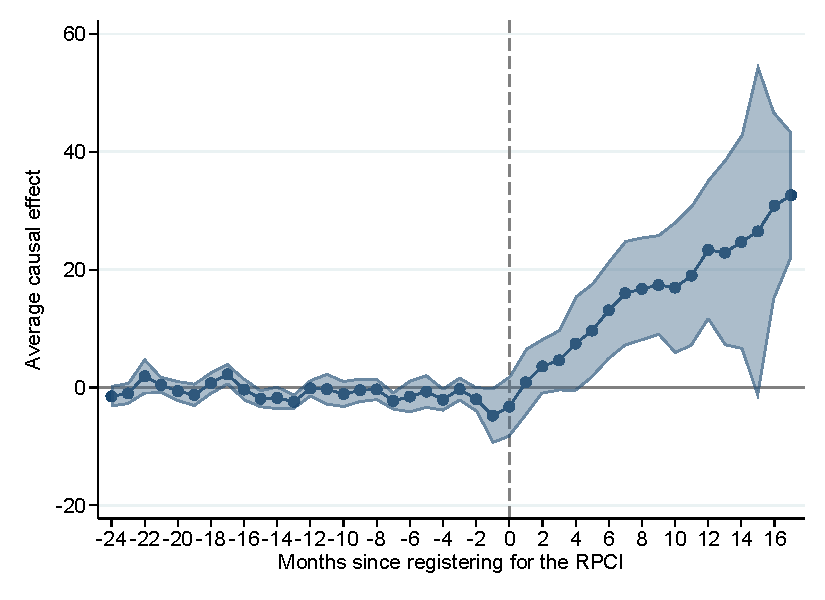
\includegraphics[width=\textwidth]{04_Figures/muestra_10porciento/event_study_sal_cierre_chaisemartin_div_final_6.pdf}
    \end{subfigure}
    \begin{subfigure}{0.49\textwidth}
    \caption{Communications and Transportation}
    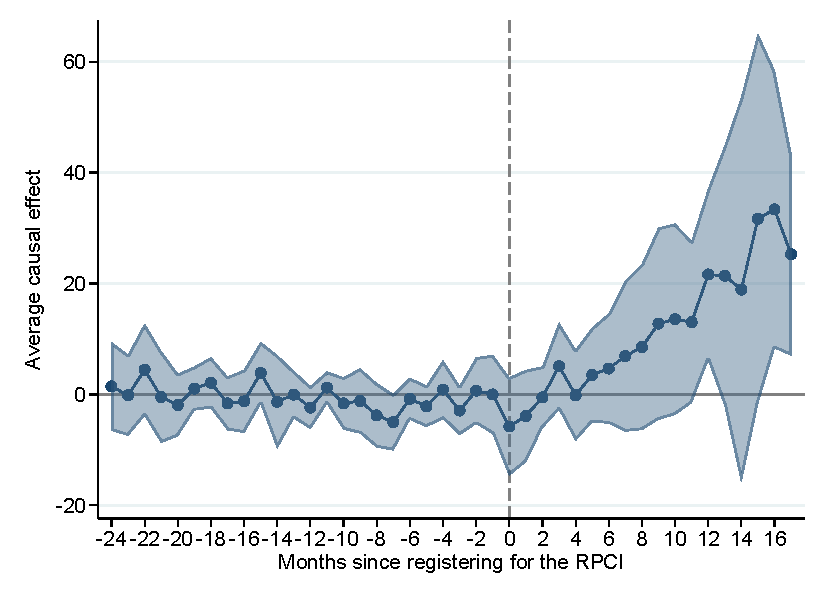
\includegraphics[width=\textwidth]{04_Figures/muestra_10porciento/event_study_sal_cierre_chaisemartin_div_final_7.pdf}
    \end{subfigure}
    
    %\textit{Do file: did_multiplegt_heterogeneity_rpci.do}
    \end{center}
\end{figure}
\scriptsize{
\noindent \textit{Sample:} 10\% of the workers registered at the Mexican Institute of Social Security (IMSS) between January 2020 and August 2022. The graphs use the estimators proposed by Chaisemartin and D'Haultfoeuille to prevent posible negative weights in the Difference in Differences estimators. Each subfigure conditions on firm characteristics at baseline, during 2020, previous to the RPCI launch. Columns (a) to (f) condition on the firm industry: (a) transformation industry, (b) construction industry, (c) commerce, (d) communications and transportation, (e) services for firms and people, (f) communal and social services. Column (g) and (h) condition on firm size categories: (g) small firms (less than 250 workers), (h) big firms (more than 1000 workers).
}

\clearpage

\begin{figure}[H]
    \ContinuedFloat
    \caption{(Continued) Event studies - RPCI effect on wage by firm characteristics}
    \label{event_study_wage_firm_characteristics_cont}
    \begin{center}

    \begin{subfigure}{0.49\textwidth}
    \caption{Services for Firms and People}
    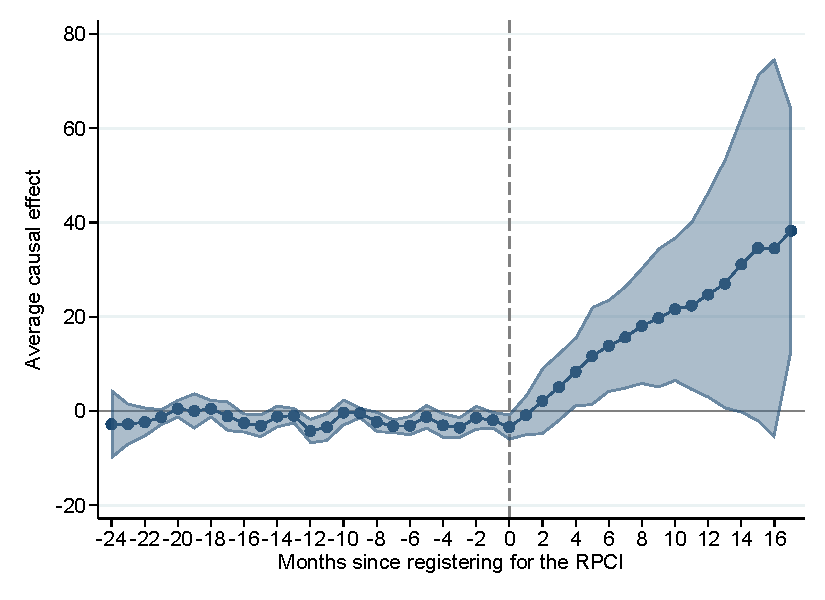
\includegraphics[width=\textwidth]{04_Figures/muestra_10porciento/event_study_sal_cierre_chaisemartin_div_final_8.pdf}
    \end{subfigure}
    \begin{subfigure}{0.49\textwidth}
    \caption{Social and Communal Services}
    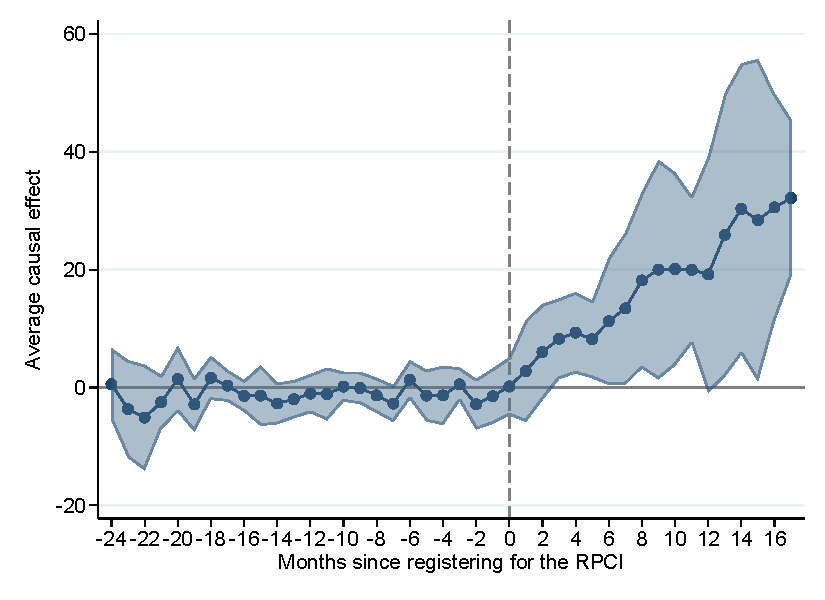
\includegraphics[width=\textwidth]{04_Figures/muestra_10porciento/event_study_sal_cierre_chaisemartin_div_final_9.pdf}
    \end{subfigure}
    
    \begin{subfigure}{0.49\textwidth}
    \caption{Small Firms}
    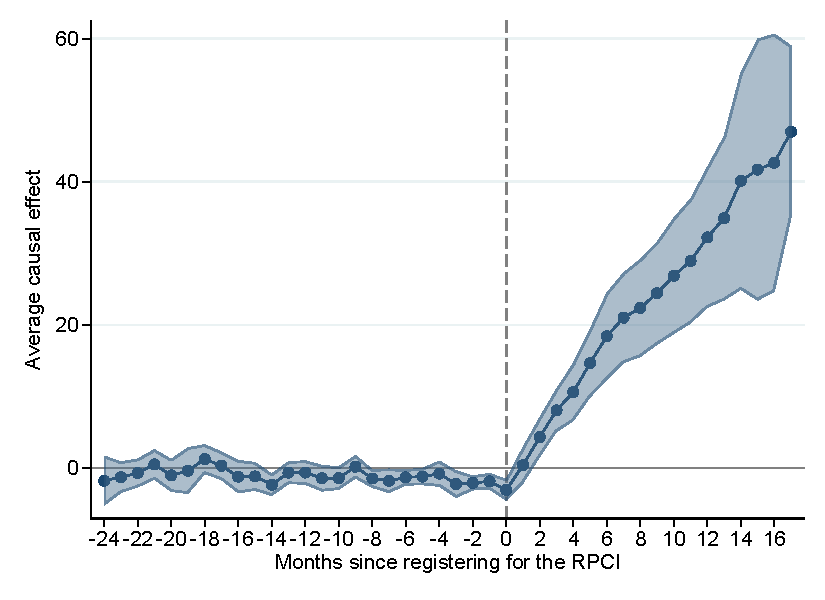
\includegraphics[width=\textwidth]{04_Figures/muestra_10porciento/event_study_sal_cierre_chaisemartin_pyme.pdf}
    \end{subfigure}
    \begin{subfigure}{0.49\textwidth}
    \caption{Big Firms}
    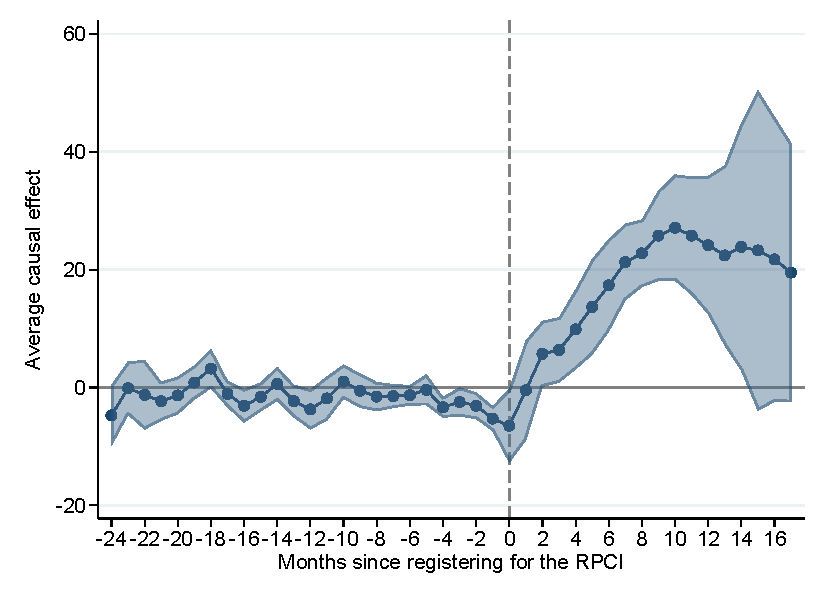
\includegraphics[width=\textwidth]{04_Figures/muestra_10porciento/event_study_sal_cierre_chaisemartin_emp_grande.pdf}
    \end{subfigure}
    
    %\textit{Do file: did_multiplegt_heterogeneity_rpci.do}
    \end{center}
\end{figure}

\scriptsize{
\noindent \textit{Sample:} 10\% of the workers registered at the Mexican Institute of Social Security (IMSS) between January 2020 and August 2022. The graphs use the estimators proposed by Chaisemartin and D'Haultfoeuille to prevent posible negative weights in the Difference in Differences estimators. Each subfigure conditions on firm characteristics at baseline, during 2020, previous to the RPCI launch. Subfigures (a) to (f) condition on the firm industry: (a) transformation industry, (b) construction industry, (c) commerce, (d) communications and transportation, (e) services for firms and people, (f) communal and social services. Subfigures (g) and (h) condition on firm size categories: (g) small firms (less than 250 workers), (h) big firms (more than 1000 workers).
}

\clearpage

\begin{figure}[H]
    \caption{Event studies - RPCI effect on log wage by firm characteristics}
    \label{event_study_log_wage_firm_characteristics}
    \begin{center}
    
    \begin{subfigure}{0.49\textwidth}
    \caption{Transformation Industry}
    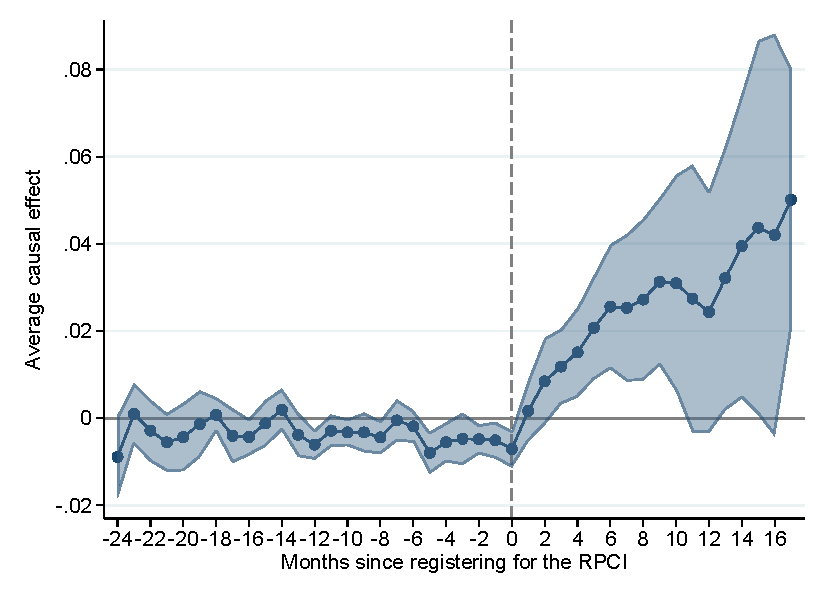
\includegraphics[width=\textwidth]{04_Figures/muestra_10porciento/event_study_log_sal_cierre_chaisemartin_div_final_3.pdf}
    \end{subfigure}
    \begin{subfigure}{0.49\textwidth}
    \caption{Construction Industry}
    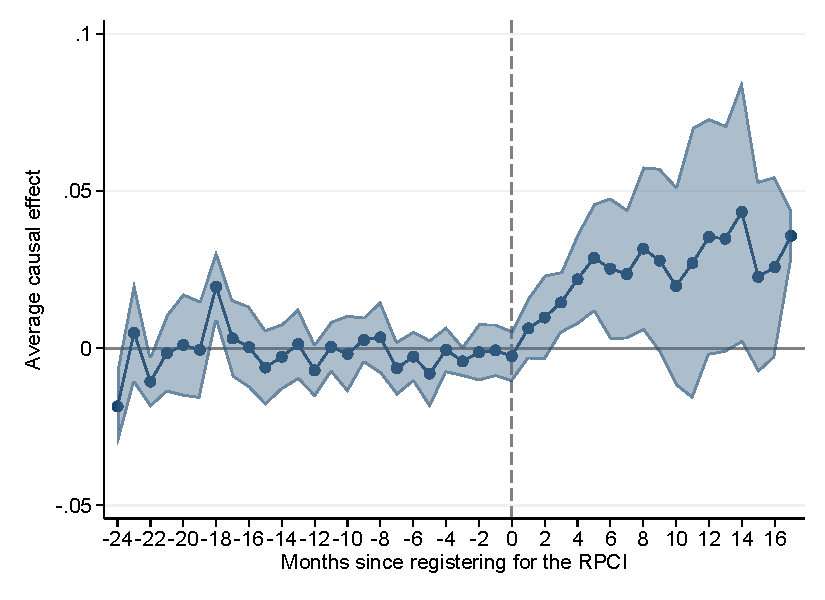
\includegraphics[width=\textwidth]{04_Figures/muestra_10porciento/event_study_log_sal_cierre_chaisemartin_div_final_4.pdf}
    \end{subfigure}
    
    \begin{subfigure}{0.49\textwidth}
    \caption{Commerce}
    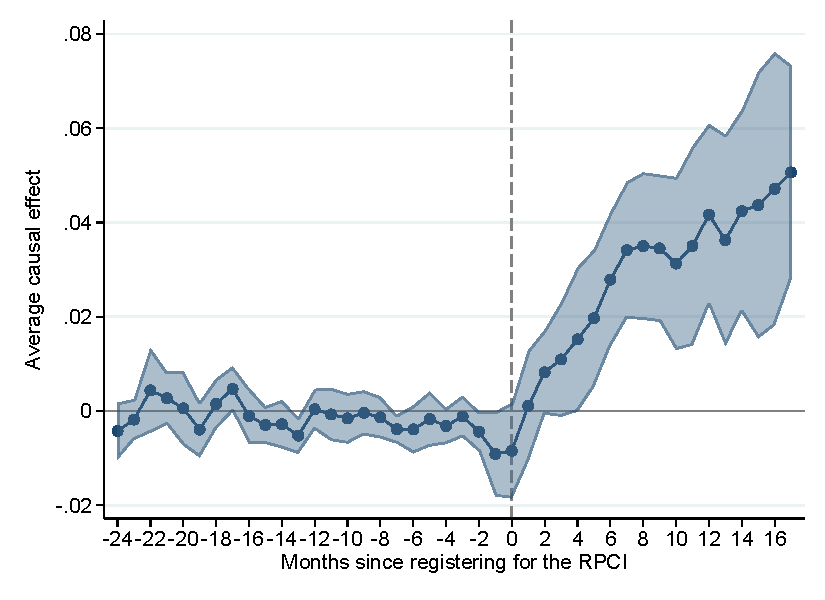
\includegraphics[width=\textwidth]{04_Figures/muestra_10porciento/event_study_log_sal_cierre_chaisemartin_div_final_6.pdf}
    \end{subfigure}
    \begin{subfigure}{0.49\textwidth}
    \caption{Communications and Transportation}
    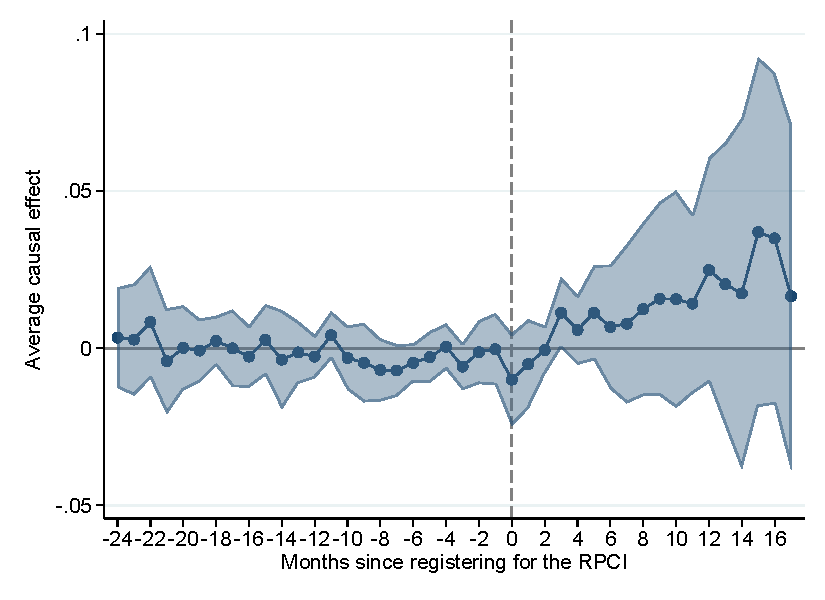
\includegraphics[width=\textwidth]{04_Figures/muestra_10porciento/event_study_log_sal_cierre_chaisemartin_div_final_7.pdf}
    \end{subfigure}
    
    %\textit{Do file: did_multiplegt_heterogeneity_rpci.do}
    \end{center}
\end{figure}
\scriptsize{
\noindent \textit{Sample:} 10\% of the workers registered at the Mexican Institute of Social Security (IMSS) between January 2020 and August 2022. The graphs use the estimators proposed by Chaisemartin and D'Haultfoeuille to prevent posible negative weights in the Difference in Differences estimators. Each subfigure conditions on firm characteristics at baseline, during 2020, previous to the RPCI launch. Columns (a) to (f) condition on the firm industry: (a) transformation industry, (b) construction industry, (c) commerce, (d) communications and transportation, (e) services for firms and people, (f) communal and social services. Column (g) and (h) condition on firm size categories: (g) small firms (less than 250 workers), (h) big firms (more than 1000 workers).
}

\clearpage

\begin{figure}[H]
    \ContinuedFloat
    \caption{(Continued) Event studies - RPCI effect on log wage by firm characteristics}
    \label{event_study_log_wage_firm_characteristics_cont}
    \begin{center}

    \begin{subfigure}{0.49\textwidth}
    \caption{Services for Firms and People}
    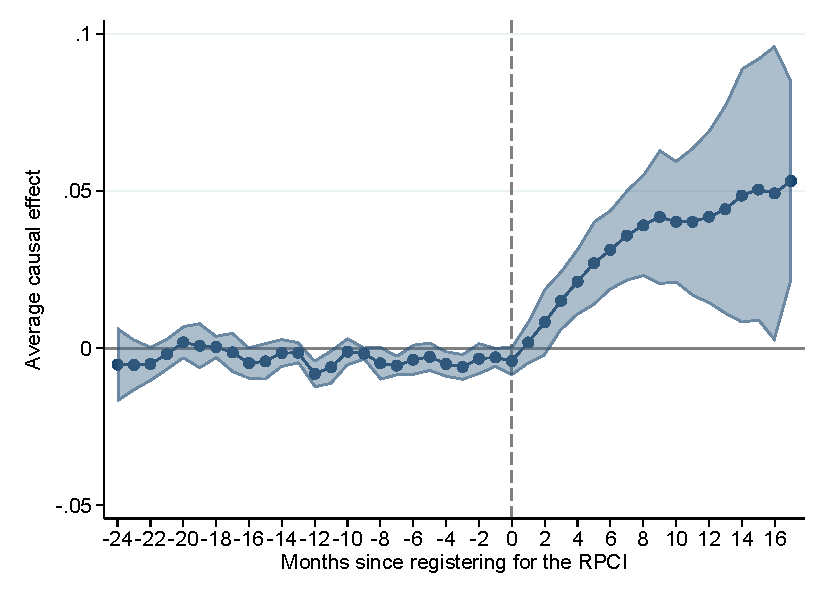
\includegraphics[width=\textwidth]{04_Figures/muestra_10porciento/event_study_log_sal_cierre_chaisemartin_div_final_8.pdf}
    \end{subfigure}
    \begin{subfigure}{0.49\textwidth}
    \caption{Social and Communal Services}
    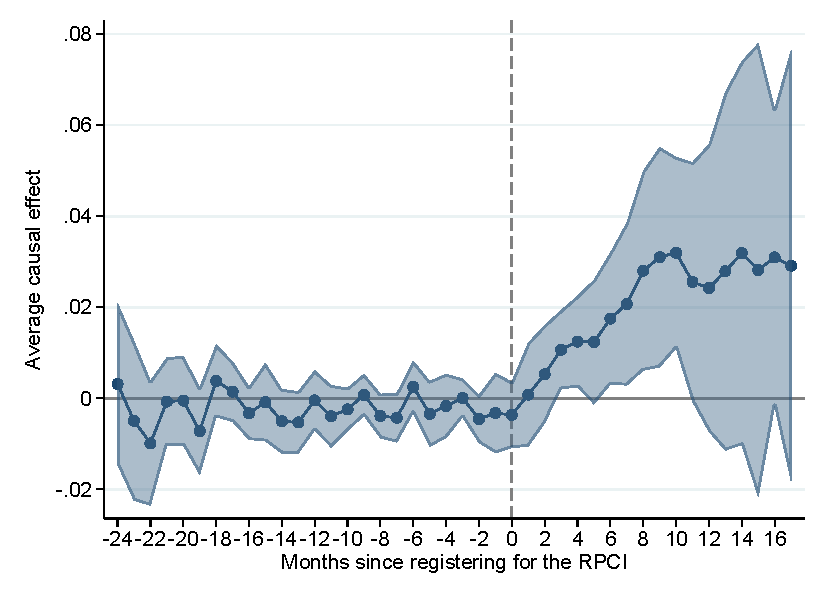
\includegraphics[width=\textwidth]{04_Figures/muestra_10porciento/event_study_log_sal_cierre_chaisemartin_div_final_9.pdf}
    \end{subfigure}
    
    \begin{subfigure}{0.49\textwidth}
    \caption{Small Firms}
    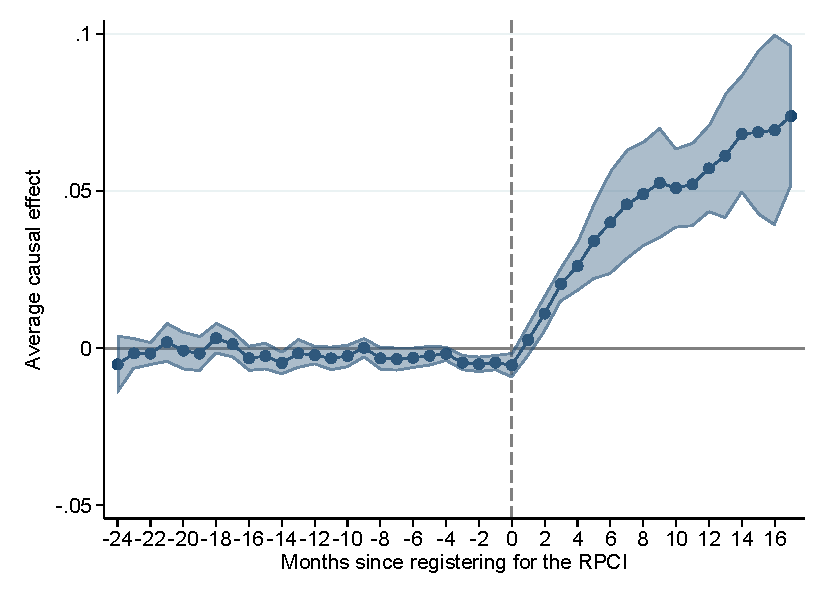
\includegraphics[width=\textwidth]{04_Figures/muestra_10porciento/event_study_log_sal_cierre_chaisemartin_pyme.pdf}
    \end{subfigure}
    \begin{subfigure}{0.49\textwidth}
    \caption{Big Firms}
    \includegraphics[width=\textwidth]{04_Figures/muestra_10porciento/event_study_log_sal_cierre_chaisemartin_emp_grande.pdf}
    \end{subfigure}
    
    %\textit{Do file: did_multiplegt_heterogeneity_rpci.do}
    \end{center}
\end{figure}

\scriptsize{
\noindent \textit{Sample:} 10\% of the workers registered at the Mexican Institute of Social Security (IMSS) between January 2020 and August 2022. The graphs use the estimators proposed by Chaisemartin and D'Haultfoeuille to prevent posible negative weights in the Difference in Differences estimators. Each subfigure conditions on firm characteristics at baseline, during 2020, previous to the RPCI launch. Subfigures (a) to (f) condition on the firm industry: (a) transformation industry, (b) construction industry, (c) commerce, (d) communications and transportation, (e) services for firms and people, (f) communal and social services. Subfigures (g) and (h) condition on firm size categories: (g) small firms (less than 250 workers), (h) big firms (more than 1000 workers).
}

\clearpage

\begin{figure}[H]
    \caption{Event studies - RPCI effect on wage by firm size}
    \label{event_study_wage_firm_size}
    \begin{center}
    
    \begin{subfigure}{0.49\textwidth}
    \caption{1 Job}
    \includegraphics[width=\textwidth]{04_Figures/muestra_10porciento/event_study_sal_cierre_chaisemartin_firm_size_1.pdf}
    \end{subfigure}
    \begin{subfigure}{0.49\textwidth}
    \caption{2 to 5 Jobs}
    \includegraphics[width=\textwidth]{04_Figures/muestra_10porciento/event_study_sal_cierre_chaisemartin_firm_size_2.pdf}
    \end{subfigure}
    
    \begin{subfigure}{0.49\textwidth}
    \caption{6 to 50 Jobs}
    \includegraphics[width=\textwidth]{04_Figures/muestra_10porciento/event_study_sal_cierre_chaisemartin_firm_size_3.pdf}
    \end{subfigure}
    \begin{subfigure}{0.49\textwidth}
    \caption{51 to 250 Jobs}
    \includegraphics[width=\textwidth]{04_Figures/muestra_10porciento/event_study_sal_cierre_chaisemartin_firm_size_4.pdf}
    \end{subfigure}
    
    %\textit{Do file: did_multiplegt_heterogeneity_rpci.do}
    \end{center}
\end{figure}
\scriptsize{
\noindent \textit{Sample:} 10\% of the workers registered at the Mexican Institute of Social Security (IMSS) between January 2020 and August 2022. The graphs use the estimators proposed by Chaisemartin and D'Haultfoeuille to prevent posible negative weights in the Difference in Differences estimators.  Each subfigure conditions on firm size at baseline, during 2020, previous to the RPCI launch: (a) 1 job, (b) 2 to 5 jobs, (c) 6 to 50 jobs, (d) 51 to 250 jobs, (e) 251 to 500 jobs, (f) 501 to 1000 jobs, (g) more than 1000 jobs.
}


\clearpage

\begin{figure}[H]
    \ContinuedFloat
    \caption{(Continued) Event studies - RPCI effect on wage by firm characteristics}
    \label{event_study_wage_firm_size_cont}
    \begin{center}

    \begin{subfigure}{0.49\textwidth}
    \caption{251 to 500 Jobs}
    \includegraphics[width=\textwidth]{04_Figures/muestra_10porciento/event_study_sal_cierre_chaisemartin_firm_size_5.pdf}
    \end{subfigure}
    \begin{subfigure}{0.49\textwidth}
    \caption{501 to 1000 Jobs}
    \includegraphics[width=\textwidth]{04_Figures/muestra_10porciento/event_study_sal_cierre_chaisemartin_firm_size_6.pdf}
    \end{subfigure}
    
    \begin{subfigure}{0.49\textwidth}
    \caption{1000+ Jobs}
    \includegraphics[width=\textwidth]{04_Figures/muestra_10porciento/event_study_sal_cierre_chaisemartin_firm_size_7.pdf}
    \end{subfigure}
    
    %\textit{Do file: did_multiplegt_heterogeneity_rpci.do}
    \end{center}
\end{figure}

\scriptsize{
\noindent \textit{Sample:} 10\% of the workers registered at the Mexican Institute of Social Security (IMSS) between January 2020 and August 2022. The graphs use the estimators proposed by Chaisemartin and D'Haultfoeuille to prevent posible negative weights in the Difference in Differences estimators.  Each subfigure conditions on firm size at baseline, during 2020, previous to the RPCI launch: (a) 1 job, (b) 2 to 5 jobs, (c) 6 to 50 jobs, (d) 51 to 250 jobs, (e) 251 to 500 jobs, (f) 501 to 1000 jobs, (g) more than 1000 jobs.
}

\clearpage

\begin{figure}[H]
    \caption{Event studies - RPCI effect on log wage by firm size}
    \label{event_study_log_wage_firm_size}
    \begin{center}
    
    \begin{subfigure}{0.49\textwidth}
    \caption{1 Job}
    \includegraphics[width=\textwidth]{04_Figures/muestra_10porciento/event_study_log_sal_cierre_chaisemartin_firm_size_1.pdf}
    \end{subfigure}
    \begin{subfigure}{0.49\textwidth}
    \caption{2 to 5 Jobs}
    \includegraphics[width=\textwidth]{04_Figures/muestra_10porciento/event_study_log_sal_cierre_chaisemartin_firm_size_2.pdf}
    \end{subfigure}
    
    \begin{subfigure}{0.49\textwidth}
    \caption{6 to 50 Jobs}
    \includegraphics[width=\textwidth]{04_Figures/muestra_10porciento/event_study_log_sal_cierre_chaisemartin_firm_size_3.pdf}
    \end{subfigure}
    \begin{subfigure}{0.49\textwidth}
    \caption{51 to 250 Jobs}
    \includegraphics[width=\textwidth]{04_Figures/muestra_10porciento/event_study_log_sal_cierre_chaisemartin_firm_size_4.pdf}
    \end{subfigure}
    
    %\textit{Do file: did_multiplegt_heterogeneity_rpci.do}
    \end{center}
\end{figure}
\scriptsize{
\noindent \textit{Sample:} 10\% of the workers registered at the Mexican Institute of Social Security (IMSS) between January 2020 and August 2022. The graphs use the estimators proposed by Chaisemartin and D'Haultfoeuille to prevent posible negative weights in the Difference in Differences estimators.  Each subfigure conditions on firm size at baseline, during 2020, previous to the RPCI launch: (a) 1 job, (b) 2 to 5 jobs, (c) 6 to 50 jobs, (d) 51 to 250 jobs, (e) 251 to 500 jobs, (f) 501 to 1000 jobs, (g) more than 1000 jobs.
}


\clearpage

\begin{figure}[H]
    \ContinuedFloat
    \caption{(Continued) Event studies - RPCI effect on log wage by firm characteristics}
    \label{event_study_log_wage_firm_size_cont}
    \begin{center}

    \begin{subfigure}{0.49\textwidth}
    \caption{251 to 500 Jobs}
    \includegraphics[width=\textwidth]{04_Figures/muestra_10porciento/event_study_log_sal_cierre_chaisemartin_firm_size_5.pdf}
    \end{subfigure}
    \begin{subfigure}{0.49\textwidth}
    \caption{501 to 1000 Jobs}
    \includegraphics[width=\textwidth]{04_Figures/muestra_10porciento/event_study_log_sal_cierre_chaisemartin_firm_size_6.pdf}
    \end{subfigure}
    
    \begin{subfigure}{0.49\textwidth}
    \caption{1000+ Jobs}
    \includegraphics[width=\textwidth]{04_Figures/muestra_10porciento/event_study_log_sal_cierre_chaisemartin_firm_size_7.pdf}
    \end{subfigure}
    
    %\textit{Do file: did_multiplegt_heterogeneity_rpci.do}
    \end{center}
\end{figure}

\scriptsize{
\noindent \textit{Sample:} 10\% of the workers registered at the Mexican Institute of Social Security (IMSS) between January 2020 and August 2022. The graphs use the estimators proposed by Chaisemartin and D'Haultfoeuille to prevent posible negative weights in the Difference in Differences estimators.  Each subfigure conditions on firm size at baseline, during 2020, previous to the RPCI launch: (a) 1 job, (b) 2 to 5 jobs, (c) 6 to 50 jobs, (d) 51 to 250 jobs, (e) 251 to 500 jobs, (f) 501 to 1000 jobs, (g) more than 1000 jobs.
}

\clearpage

\begin{figure}[H]
    \caption{Worker Survey Graphs}
    \label{worker_survey_1}
    \begin{center}

    \begin{subfigure}{0.49\textwidth}
    \includegraphics[width=\textwidth]{04_Figures/worker_survey/Exp_1.png}
    \end{subfigure}
    \begin{subfigure}{0.49\textwidth}
    \includegraphics[width=\textwidth]{04_Figures/worker_survey/Exp_2.png}
    \end{subfigure}
    
    \begin{subfigure}{0.49\textwidth}
    \includegraphics[width=\textwidth]{04_Figures/worker_survey/Exp_3.png}
    \end{subfigure}
    \begin{subfigure}{0.49\textwidth}
    \includegraphics[width=\textwidth]{04_Figures/worker_survey/Exp_4.png}
    \end{subfigure}
    
    \begin{subfigure}{0.49\textwidth}
    \includegraphics[width=\textwidth]{04_Figures/worker_survey/Exp_5.png}
    \end{subfigure}
    \begin{subfigure}{0.49\textwidth}
    \includegraphics[width=\textwidth]{04_Figures/worker_survey/Exp_6.png}
    \end{subfigure}
    
    \end{center}
\end{figure}

\clearpage

\begin{figure}[H]
    \caption{Worker Survey Graphs}
    \label{worker_survey_2}
    \begin{center}

    \begin{subfigure}{0.49\textwidth}
    \includegraphics[width=\textwidth]{04_Figures/worker_survey/Exp_7.png}
    \end{subfigure}
    \begin{subfigure}{0.49\textwidth}
    \includegraphics[width=\textwidth]{04_Figures/worker_survey/Exp_8.png}
    \end{subfigure}
    
    \begin{subfigure}{0.49\textwidth}
    \includegraphics[width=\textwidth]{04_Figures/worker_survey/Exp_9.png}
    \end{subfigure}
    \begin{subfigure}{0.49\textwidth}
    \includegraphics[width=\textwidth]{04_Figures/worker_survey/Exp_10.png}
    \end{subfigure}
    
    \begin{subfigure}{0.49\textwidth}
    \includegraphics[width=\textwidth]{04_Figures/worker_survey/Exp_11.png}
    \end{subfigure}
    \begin{subfigure}{0.49\textwidth}
    \includegraphics[width=\textwidth]{04_Figures/worker_survey/Exp_12.png}
    \end{subfigure}
    
    \end{center}
\end{figure}

\clearpage

\begin{figure}[H]
    \caption{Worker Survey Graphs}
    \label{worker_survey_3}
    \begin{center}

    \begin{subfigure}{0.49\textwidth}
    \includegraphics[width=\textwidth]{04_Figures/worker_survey/Exp_13.png}
    \end{subfigure}
    \begin{subfigure}{0.49\textwidth}
    \includegraphics[width=\textwidth]{04_Figures/worker_survey/Exp_14.png}
    \end{subfigure}
    
    \begin{subfigure}{0.49\textwidth}
    \includegraphics[width=\textwidth]{04_Figures/worker_survey/Exp_15.png}
    \end{subfigure}
    \begin{subfigure}{0.49\textwidth}
    \includegraphics[width=\textwidth]{04_Figures/worker_survey/Exp_16.png}
    \end{subfigure}
    
    \end{center}
\end{figure}


%%%%%%%%%%%%%%%%%%%%%%%%%%%%%%%%%%%%%%%%%%%%%%%%%%%%%%

\newpage
%  \documentclass[oneside,11pt]{article}

% 
\usepackage{soul}
\usepackage{natbib}
\usepackage{hyperref}
\usepackage{bookmark}
\usepackage{graphicx}             
\graphicspath{{./Figuras/}}
\usepackage[dvipsnames]{xcolor}
\usepackage{todonotes}
\usepackage{makecell}
\usepackage[margin=1in]{geometry}
\usepackage{float}                
\usepackage{amsmath}
\usepackage{amscd}
\usepackage{amsfonts}
\usepackage{amssymb}
\usepackage{bbm}
\usepackage{booktabs}
\usepackage{nameref}
\usepackage{multirow}
\usepackage[nokeyprefix]{refstyle}
\usepackage{rotating}
\usepackage{threeparttable}
\usepackage{afterpage}
\usepackage{lscape}
\usepackage{enumerate}
\usepackage{caption}
\usepackage{subcaption}
\usepackage{epstopdf}
\usepackage{setspace}
\usepackage{svg}
\usepackage{dsfont}
\usepackage{amsthm}
\usepackage{tocloft}
\usepackage{etoc}
\usepackage{lmodern}
\usepackage{bm}
\usepackage[T1]{fontenc}
\usepackage{tgpagella}

\epstopdfDeclareGraphicsRule{.tiff}{png}{.png}{convert #1 \OutputFile}
\AppendGraphicsExtensions{.tiff}

\epstopdfDeclareGraphicsRule{.tif}{png}{.png}{convert #1 \OutputFile}
\AppendGraphicsExtensions{.tif}

\def\sym#1{\ifmmode^{#1}\else\(^{#1}\)\fi}

\usepackage{tikz}
\usetikzlibrary{shapes.geometric, arrows}
\usetikzlibrary{calc}
\usetikzlibrary{matrix}

\tikzset{ 
    table/.style={
        matrix of nodes,
        row sep=-\pgflinewidth,
        column sep=-\pgflinewidth,
        nodes={
            rectangle,
            draw=black,
            align=center
        },
        minimum height=1.5em,
        text depth=0.5ex,
        text height=2ex,
        nodes in empty cells,
%%
        every even row/.style={
            nodes={fill=gray!20}
        },
        column 1/.style={
            nodes={text width=2em,font=\bfseries}
        },
        row 1/.style={
            nodes={
                fill=black,
                text=white,
                font=\bfseries
            }
        }
    }
}


\usepackage{colortbl}
\usepackage{url}
\urlstyle{rm}
\definecolor{darkblue}{rgb}{0,0,.4}
\hypersetup{colorlinks=true, breaklinks=true, citecolor=Maroon, linkcolor=darkblue, menucolor=darkblue, urlcolor=darkblue}

\newtheorem{theorem}{Theorem}
\newtheorem{claim}[theorem]{Claim}
\newtheorem{prop}[theorem]{Proposition} 
\newtheorem{cor}[theorem]{Corollary} 
\newtheorem{assumption}{Assumption} 
\newtheorem{lem}{Lemma} 

\DeclareRobustCommand{\hlgr}[1]{{\sethlcolor{green}\hl{#1}}}


\usepackage{comment}
%para esconder columnas en tablas (enrique)
\usepackage{array}
\newcolumntype{H}{>{\setbox0=\hbox\bgroup}c<{\egroup}@{}}
\linespread{1.25}

\newcommand{\wh}{\widehat}
\usepackage{anyfontsize}

\usepackage[linesnumbered,vlined,ruled,commentsnumbered]{algorithm2e}

\DontPrintSemicolon
\newcommand{\To}{\mbox{\upshape\bfseries to}}
\newcommand{\E}{\mathbb{E}}

\DeclareCaptionFormat{cont}{#1 (cont.)#2#3\par}
% %%% HELPER CODE FOR DEALING WITH EXTERNAL REFERENCES
% \usepackage{xr}
% \makeatletter
% \newcommand*{\addFileDependency}[1]{
%   \typeout{(#1)}
%   \@addtofilelist{#1}
%   \IfFileExists{#1}{}{\typeout{No file #1.}}
% }
% \makeatother


% \newcommand*{\myexternaldocument}[1]{
%     \externaldocument{#1}
%     \addFileDependency{#1.tex}
%     \addFileDependency{#1.aux}
% }

% %\myexternaldocument{OA}

% %%%%%%%%%%%%%%%%%%%%%%%%%%%%%%%% DOCUMENT
% \begin{document}

%%%%%%%%%%%%%%%%%%%%%%%%%%%%%%%%%%%%%%%%%%%%%%%

% APPENDIX 
\setcounter{table}{0}
\setcounter{figure}{0}
\setcounter{section}{0}
\pagenumbering{gobble}


\begin{center}
	\LARGE IMSS RPCI \\[0.5em]
	\Large{Appendix $-$ For Online Publication} \\[1em]
	\large \author{Eduardo Alcaraz \and Gabriela López \and Luis Martínez \and Marco Medina \and Enrique Seira}
\end{center}

\appendix
\pagenumbering{arabic}
\renewcommand\thefigure{OA-\arabic{figure}}
\renewcommand\thetable{OA-\arabic{table}}
\renewcommand*{\thepage}{OA - \arabic{page}}
\renewcommand\thesection{Appendix \Alph{section}.}
\renewcommand\thesubsection{\Alph{section}.\arabic{subsection}}

%\renewcommand{\cftparskip}{0em} % NOT NEEDED
\renewcommand\cftsecdotsep{\cftdotsep}
\renewcommand\cftsubsecdotsep{\cftnodots}
\renewcommand{\cftsecnumwidth}{6em}
 \renewcommand{\cftpnumalign}{r}
%\renewcommand{\cftsecleader}{\normalfont\cftdotfill{\cftsecdotsep}}


\renewcommand{\cftsecleader}{\cftdotfill{\cftsecdotsep}\hspace{1.8em}}
%\renewcommand{\cftsecpagefont}{20em}
%\renewcommand{\cftfignumwidth}{6em}
%\renewcommand{\cfttabnumwidth}{3.3em}

%\tableofcontents
\etocdepthtag.toc{mtappendix}
\etocsettagdepth{mtchapter}{none}
\etocsettagdepth{mtappendix}{subsection}

\setstretch{0.9}
%\renewcommand\contentsname{} % the empty name

\begingroup
\let\clearpage\relax
%\vspace{-1.5em} % the removed space. Set as appropriate
\tableofcontents
\endgroup

\clearpage

\section{ RPCI}
\vspace{.2in}

\begin{figure}[H]
    \caption{RPCI flyers}
    \label{rpci_flyers}
    \begin{center}
    
    \begin{subfigure}{0.49\textwidth}
    \caption{RPCI flyer titled "Does my employer has me registered at IMSS?"}
    \includegraphics[width=\textwidth]{04_Figures/rpci_app/rpci_flyer_3.jpeg}
    \end{subfigure}
    \begin{subfigure}{0.49\textwidth}
    \caption{RPCI flyer titled "Digital services for a healthy environment"}
    \includegraphics[width=\textwidth]{04_Figures/rpci_app/rpci_flyer_2.jpeg}
    \end{subfigure}

    \end{center}
\end{figure}
\scriptsize{
\noindent Flyers circulated by the Mexican Institute of Social Security (IMSS) for the RPCI. Both flyers explain how you can track and access your job register information, such as wage and firm you are registered at, if you register for the RPCI.
}

\clearpage

\begin{figure}[H]
    \caption{Registering for the RPCI}
    \label{rpci_register}
    \begin{center}
    
    \begin{subfigure}{0.9\textwidth}
    \includegraphics[width=\textwidth]{04_Figures/rpci_app/rpci_register.png}
    \end{subfigure}

    \end{center}
\end{figure}
\scriptsize{
\noindent Diagram shows how to register for the RPCI within the IMSS Digital app. The worker registers only once to access the RPCI, using his Unique Population Registry Key (CURP) and email address.
}

\clearpage

\begin{figure}[H]
    \caption{RPCI example}
    \label{rpci_example}
    \begin{center}
    
    \begin{subfigure}{0.49\textwidth}
    \caption{RPCI within the IMSS Digital app}
    \includegraphics[width=\textwidth]{04_Figures/rpci_app/rpci_2.png}
    \end{subfigure}
    \begin{subfigure}{0.49\textwidth}
    \caption{RPCI PDF file}
    \includegraphics[width=\textwidth]{04_Figures/rpci_app/rpci_3.png}
    \end{subfigure}
    

    \end{center}
\end{figure}
\scriptsize{
\noindent Figure (a) shows the IMSS Digital app, where once the worker is registered for the RPCI, the worker can download their report in PDF or receive it via email. Figure (b) shows an example of the PDF for the RPCI. The report includes the worker job registered information, such as wage and the firm the worker is registered at.
}

%\clearpage

%\bibliographystyle{authordate1}
%\bibliographystyle{amsalpha}
%\bibliographystyle{AER}

%\bibliography{References}




% \end{document}

\end{document}

